\documentclass[12pt,a4paper]{article}
\usepackage{graphicx}
\usepackage{tabularx}
\usepackage{array}
\usepackage{blindtext}
\usepackage{titlesec}
\usepackage[utf8]{inputenc}
\usepackage{geometry}
\usepackage{ragged2e}
\usepackage{longtable}
 \geometry{
 a4paper,
 total={170mm,257mm},
 left=19mm,
 top=19mm,
 bottom=19mm,
 right=19mm
 }
\begin{document}
%--------------Title Page ------------------
\thispagestyle{empty}
\begin{center}
\textbf{\large{Merchant Monetary System}}\\
\vspace{1cm}
\textbf{ Final Report} \\
\vspace{2cm}

\includegraphics[scale=.08]{UETLogo}\\
\vspace{2cm}
\underline{ Project Supervisor}\\
\vspace{1cm}
Mr. Samyan Qayyum Wahla\\
\vspace{1cm}
\underline {Group ID $(G 11)$} \\
\vspace{1cm}
Project Member\\
\vspace{0.5cm}
\begin{tabular}{ m{5cm} m{4cm}}
 Syed Hashir & 2021-CS-1 \\ 
 Kabir Ahmed & 2021-CS-4  \\  
 M. Hamad Hassan & 2021-CS-33
\end{tabular}
\vspace{5.5cm}
\par\rule{\textwidth}{0.5pt} 
Department of Computer Science\\
University of Engineering and Technology, Lahore\\
Pakistan
\end{center}
%-----------------Table of Content-----------------------
\tableofcontents
\thispagestyle{empty}
\pagenumbering{arabic}

\newpage
\setcounter{page}{1}
%-------------------------------------------------------
%----------------ProjectDescription --------------------
\justifying
\section{Project Description}

The system is designed for a company that provides
logistics (delivery of products to its client), product management (crud operations), and effective communication with their worker, clients, and vendors.
 
The company has its office, warehouse, and rider. 
It has a different contract with multiple firms to take the shipment from the vendors and store it in dedicated warehouses. The rider will take orders from the shopkeeper. Their order is received at the office, and the office will create the feasibility report according to their shopkeepers' needs and instructions generated for their warehouse manager to fulfill their order. The area-specific rider will receive an email about their order. The office will send a confirmation email to their shopkeeper. 
 
There are a total of four actors in the system and two stakeholders. Their titles and roles are:
\begin{itemize}
\item \textbf{ CEO:} The company's owner manages all the operations.
\item \textbf{Employee:} They are assistants to CEO to help in company operations. 
\item \textbf{Warehouse Manager:} Received the instructions from the employee and ready the shipment for the rider, and managed other expenses.
\item \textbf{Rider:} They take orders from different shopkeepers and deliver the product according to pre-subscribed routes defined by the system.
\end{itemize}
The stakeholder is:
\begin{itemize}
\item \textbf{Shopkeepers:} Getting the goods and services from the company.
\item \textbf{Vendor:} The vendor will provide the products to the company. 
\end{itemize}
This system is designed for one company and one CEO. CEO will be provided with already defined credentials. The CEO is responsible for creating accounts for all others actors. The CEO will provide a credential to the actors, and they will be able to update their credentials. 
 
The first dedicated dashboard for the CEO, where they monitor all operations. The operations manage their workers, products, and expenses and send emails. The CEO is the only person in the system with access to all operations. CEO analyzes company operations, including the performance of their workers and inventory. The system will present the company expenditure report.
 
The second dashboard is for office employees. They have access to manage emails, shopkeepers' orders, vendors' shipments, and company expenses. The company's expenses are the CEO, rider, and warehouse salaries. The system will present the report of payment to the vendor and shopkeeper. An employee will enter all the shipments that the company receives. They add product identifiers.
 
The third dashboard is for the warehouse manager, who receives feasibility reports of office employees and prepares the order for the rider. The warehouse manager must record the labor used in preparing the order. It could provide the miscellaneous expenses of the warehouse, like electricity costs, etc. They can view the product and make suitable changes according to the requirements.
 
The fourth dashboard is for a rider, which is basically the communicator between the company and the shopkeeper.
The rider is responsible for taking orders from the shopkeeper. 
Enter order details into the system. 
The riders will check the current orders assigned to them by the company. They will pick up the shipment from the warehouse and delivery them to the shopkeeper. The system will present the routes to the destination with the order detail. The rider received a specific amount of fuel to perform the operations. The prescribed fuel is calculated according to the formula. They can see all the products. The product will be sorted in any order. Search for a specific product from a wide range of available products. The system will deploy different sharp algorithms to access the desired date orders quickly. Able to place the order and view the detail of the order as well. 
 
The system will present the report to the CEO according to the performance of their workers, expenditures, sales and profit, salaries, inventory report, riders' performance, shopkeeper and vendor payment, workers' report, individual warehouse report, and miscellaneous expenses.
Like how many products are received in the warehouse, how many products are left, how many products are delivered to company clients, how many riders have done shipments, which rider performs most shipments, and which rider needs to perform better. It also includes how many orders a shopkeeper placed and whether the company received the payment. 
 
The email notification mechanism is embedded in the system, which helps the company communicate within and outside with other vendors and shopkeepers. After the rider has confirmed the order, the system will send an email to the company. The company will send the order details to the warehouse manager to prepare the shipment for the rider. The rider also received the email for the delivery of the order. The employee emails the CEO for any need of assistance with an issue. The warehouse manager and rider also mail to the company office for any assistance. In external communication, the client will receive a confirmation email from the system about their order. They also take assistance from the company with any issue. 
 
All the data is stored in an effective data structure to extract the data according to the need of the system actor and stakeholder.
%-------------------------------------------------------
%-----------------------Project Fectures----------------
\section{Project Features}

\begin{enumerate}
\item CEO is able to manage employees, warehouse manager, rider, and shopkeeper.  
\item CEO and Employee manage product-related operations.
\item CEO will be able to analyze company operations.  
\item Warehouse manager readies the shipment for the rider. 
\item Rider delivered the shipment to their shopkeeper. 
\item Riders are able to select the shortest route to reach the destination.  
\item One user is able to notify other users through email.
\item Riders are able to view products and place an order. 
\item System presents different reports that will be generated.

\end{enumerate}


%-------------------------------------------------------
%-----------------------Technology Stack----------------
\newpage
\section{Technology Stack}
The system is designed, developed, and tested in a desktop application. The system used the following language, packages, and an Integrated development environment.\\
\begin{longtable}{lr} 
 \caption{Details of technology used in the system. The version number is enclosed in brackets }\\
\begin{tabular}{ | m{4cm} | m{12cm}| } 
  \hline
Language & C \#  (7.3)  \\
 \hline
 Framework & .Net framework (4.7.2) \\
 \hline
IDE  & Microsoft Visual Studio 2022
 \\ \hline
 Packages    & 
Dynamic Language Runtime (1.3.3),
Entity Framework (6.4.4),
GMap.NET.Windows (2.1.7),
Microsoft.CSharp (4.7.0),
Newtonsoft.Json (13.0.1),
Stub.System.Data.SQLite.Core.NetFramework (1.0.115.5),
System.Buffers (4.5.1),
System.Data.SqlClient (4.8.3)
System.Data.SQLite (1.0.115.5)
System.Memory (4.5.5)
System.Numerics.Vectors (4.5.0)
System.Reflection.Emit (4.3.0)
System.Runtime.CompilerServices.Unsafe (4.5.3)
System.Security.Principal.Windows (5.0.0)
 
 \\ \hline
\end{tabular}
\end{longtable}
\subsection{System Requirement}
\begin{longtable}{lr} 
 \caption{To run Merchant Monetary System, your computer must meet the minimum technical specifications outlined below. For optimum performance, use recommended system specifications.}\\
\begin{tabular}{ | m{4cm} | m{12cm}| } \hline
Processor & 
Multicore Intel® or AMD processor (2 GHz or faster processor with SSE 4.2 or later) with 64-bit support
 \\ \hline
Operating system & Windows 8
 \\ \hline
RAM & 4 GB
 \\ \hline
Monitor resolution & 1280 x 800 display at 100%
 \\ \hline
Hard disk space & 1 GB of available hard-disk space
 \\ \hline
Internet & 
An active Internet connection is required to find the routes on  map. 
  \\ \hline
\end{tabular}
\end{longtable}
%-------------------------------------------------------
%-----------------------Project Actors----------------
\section{Project Actors}
There are a total of four actors in the system and two stakeholders. Their titles and roles are:
\begin{itemize}
\item \textbf{ CEO:} The company's owner manages all the operations.
\item \textbf{Employee:} They are assistants to CEO to help in company operations. 
\item \textbf{Warehouse Manager:} Received the instructions from the employee and ready the shipment for the rider, and managed other expenses.
\item \textbf{Rider:} They take orders from different shopkeepers and deliver the product according to pre-subscribed routes defined by the system.
\end{itemize}
The stakeholders are:
\begin{itemize}
\item \textbf{Shopkeeper:} Getting the goods and services from the company.
\item \textbf{Vendor:} The vendor will provide the products to the company. 
\end{itemize}
%-------------------------------------------------------
%-----------------------Use Cases----------------
\section{Use Cases}
%------------------------------------------
\subsection{Use Case 1:Log In}
\begin{longtable}{| p{3cm}|p{12cm}|}
\multicolumn{2}{c}{}
\endfirsthead
\multicolumn{2}{c}{\tablename\ \thetable\ -- \textit{Continued from previous page}}\\
\multicolumn{2}{c}{}\\
\hline
\endhead
\hline \multicolumn{2}{r}{\tablename\ \thetable\ -- \textit{Continued on next page}} \\
\endfoot
\hline
\endlastfoot
\hline
Use Case ID & U01   \\\hline
Name  &  Login \\ \hline
Actors &   CEO, Employee, Rider, Warehouse Manager \\ \hline
Description & The login screen will be presented. The actor will select theor role and enter their username and password. And click on the login button. The system will check for its validity. The system will present the respective dashboard.
\\ \hline
Pre-Condition & The respective actor will initiate the system, and the login in form is presented.  \\
\hline
Flow & Main Success Scenario (or Basic Flow):
\begin{enumerate}
\item Actor is ready to take identifiers.
\item Actor selects his/her role from the given list.   
\item Actor enters his/her username.
\item Actor enters his/her password.
\item Actor clicks on the login button. 
\end{enumerate}
Extensions (or Alternative Flows):

 *a. If forgot password button is clicked 
 \begin{enumerate}
		\item U02 will initiate
	\end{enumerate}
 *b. If the exit button is clicked
	\begin{enumerate}
		\item System will close
	\end{enumerate}
 2a. If the actor doesn't select his/her role.
 	\begin{enumerate}
		\item Error Signal will be present.
	\end{enumerate}
3a. If the actor doesn't enter his/her username.
 	\begin{enumerate}
		\item Error Signal will be present.
	\end{enumerate}
4a. If the actor doesn't enter his/her password.
 	\begin{enumerate}
		\item Error Signal will be present.
	\end{enumerate}
5a. if the selected role doesn't exist with existing data
	\begin{enumerate}
		\item Error Signal will be present.
	\end{enumerate}
5b. if the entered username doesn't exist with existing data
	\begin{enumerate}
		\item Error Signal will be present.
	\end{enumerate}
5c. if the entered password doesn't exist with existing data
	\begin{enumerate}
		\item Error Signal will be present.
	\end{enumerate}
	%---------------------
	
\\ \hline
Post-Condition & Respective Dashboard will be presented   
\\ \hline
Assigned To &  M. Hamad Hassan
\\ \hline
Working By &    M. Hamad Hassan
\\ \hline
Status & 	Completed	
\\ \hline
Known Issues & Nil
\\\hline
\end{longtable}
%-------------------------------------------------------
\subsection{Use Case 2:Forgot Password}

\begin{longtable}{| p{3cm}|p{12cm}|}
\multicolumn{2}{c}{}
\endfirsthead
\multicolumn{2}{c}{\tablename\ \thetable\ -- \textit{Continued from previous page}}\\
\multicolumn{2}{c}{}\\
\hline
\endhead
\hline \multicolumn{2}{r}{\tablename\ \thetable\ -- \textit{Continued on next page}} \\
\endfoot
\hline
\endlastfoot
\hline

Use Case ID & U02  \\\hline

Name  	    & Forgot Password  \\ \hline

Actors     	& CEO, Employee, Rider, Warehouse Manager \\ \hline

Description & Already registered users can change their password. The actor selects their role and enters his username and password. Then the actor confirms their password and clicks on Update Button; their password will be changed. \\ \hline

Pre-Condition & User must be registered in the system. Forgot Password screen is presented.  \\ \hline
Flow & Main Success Scenario (or Basic Flow):
\begin{enumerate}
\item Actor is ready to enter the identifiers.
\item Actor selects his/her role from the given list.   
\item Actor enters his/her username.
\item Actor enters his/her password.
\item Actor confirms his/her password.
\item Actor clicks on the Update button.
\end{enumerate}
Extensions (or Alternative Flows):\\
& *a. If forgot password button is clicked \\
& \begin{enumerate}
		\item U02 will initiate
	\end{enumerate}
*b. If the reset button is clicked \\
&	\begin{enumerate}
		\item All fields will get cleared.
	\end{enumerate}

2a. If the actor doesn't select his/her role.
 	\begin{enumerate}
		\item Error Signal will be presented.
	\end{enumerate}
3a. If the actor doesn't enter his/her username.
 	\begin{enumerate}
		\item Error Signal will be present.
	\end{enumerate}
4a. If the actor doesn't enter his/her password.
 	\begin{enumerate}
		\item Error Signal will be present.
	\end{enumerate}

5a. if the selected role doesn't exist with in existing data
	\begin{enumerate}
		\item Error Signal will be present.
	\end{enumerate}
5b. if the entered username doesn't exist with in existing data
	\begin{enumerate}
		\item Error Signal will be present.
	\end{enumerate}
\\ \hline
Flow & 5c. if the entered password doesn't exist with in existing data
	\begin{enumerate}
		\item Error Signal will be present.
	\end{enumerate}
	
5d. if the password doesn't match the password that the user confirmed
	\begin{enumerate}
		\item Error Signal will be present.
	\end{enumerate}
	
\\ \hline
Post-Condition & Actor's Password Updated  
\\ \hline
Assigned To &  M. Hamad Hassan
\\ \hline
Working By &    M. Hamad Hassan
\\ \hline
Status & 	Completed	
\\ \hline
Known Issues & Nil
\\\hline

\end{longtable}

%------------------------------------------
\subsection{Use Case 3:Detail of Accounts for CEO }
\begin{longtable}{| p{3cm}|p{12cm}|}
\multicolumn{2}{c}{}
\endfirsthead
\multicolumn{2}{c}{\tablename\ \thetable\ -- \textit{Continued from previous page}}\\
\multicolumn{2}{c}{}\\
\hline
\endhead
\hline \multicolumn{2}{r}{\tablename\ \thetable\ -- \textit{Continued on next page}} \\
\endfoot
\hline
\endlastfoot
\hline

Use Case ID & U03  \\\hline

Name  	    & Detail of Account for CEO  \\ \hline

Actors     	& CEO\\ \hline

Description &  CEO can view the details of each user who have registered themselves on this system. CEO can filter out users with certain designations and certain attributes and can apply multiple filters to search out specific users and  their data. CEO can delete as well as edit users.\\ \hline

Pre-Condition &  Detail of Accounts Screen is presented. \\ \hline

Flow       & Main Scenario:

\begin{enumerate}
\item  CEO selects the designation from the given list.
\item  CEO selects the attribute from the given list. 
\item  CEO could search the data from the identifier.
\item  CEO selects the filters from the given list.
\item  CEO clicks on the Go button.
\item  CEO selects the data(any row shown in the grid )from the grid. 
\item  CEO clicks on the Edit button, and a new Edit user screen opens.
\item  CEO clicks on the Delete button.
\item  CEO clicks on the Close button.

\end{enumerate}

Extensions (or Alternative Flows):\\

& 1. If CEO did not select any designation from the drop-down. \\
& \begin{enumerate}
		\item Error Signal will be present.
	\end{enumerate}
\\ 

      & 2. If CEO did not select any attribute from the drop-down.
 	\begin{enumerate}
		\item Error Signal will be present.
	\end{enumerate}
\\ 
& 3a. If CEO did not select any designation and entered the data in the identifier to search. \\
& \begin{enumerate}
		\item The searched data will show from the first attribute.
	\end{enumerate}
\\
& 3b. If CEO did not select any Attribute and entered the data in the identifier to search. \\
& \begin{enumerate}
		\item The searched data will show from the first attribute.
	\end{enumerate}
\\ 
& 3c. If CEO did not select any designation and  Attribute and entered the data in the identifier to search. \\
& \begin{enumerate}
		\item The searched data will show from the first attribute.
	\end{enumerate}
\\ 

& 4a. If CEO did not select any Filter from the given list \\
& \begin{enumerate}
		\item No operation of the filter is applied to the data.
	\end{enumerate}
\\ 
& 4b. If CEO did not select any Attribute from the given list and select any filter  \\
& \begin{enumerate}
		\item No operation of the filter is applied to the data.
	\end{enumerate}
\\ 

& 5a. If CEO did not select any Attribute, Designation, or filter from the given list and not enter the data to be searched in identifier \\
& \begin{enumerate}
		\item Error Message box will be shown.
	\end{enumerate}
\\  
& 6. If CEO did not select any data from the grid list.  \\
& \begin{enumerate}
		\item No operation is performed.
	\end{enumerate}
\\ \hline  
& 7. If CEO did not select any data from the grid list and clicked the edit button.\\
& \begin{enumerate}
		\item No operation I performed on any data list in the grid.
            \item Message Box will be shown.
	\end{enumerate}
\\
Flow       & 8. If CEO did not select any data from the grid list and clicked the delete button.\\
 	&\begin{enumerate}
			\item No operation I performed on any data list in the grid.
            \item Message Box will be shown.
	\end{enumerate}
\\ \hline 


Post-Condition &  Data from selected row will be deleted or updated 
\\ \hline
Assigned To &  M. Hamad Hassan
\\ \hline
Working By &    M. Hamad Hassan
\\ \hline
Status & 	Completed	
\\ \hline
Known Issues & Nil
\\\hline

\end{longtable}
%------------------------------------------
%------------------------------------------
\subsection{Use Case 4:Detail of Accounts for Employee }

\begin{longtable}{| p{3cm}|p{12cm}|}
\multicolumn{2}{c}{}
\endfirsthead
\multicolumn{2}{c}{\tablename\ \thetable\ -- \textit{Continued from previous page}}\\
\multicolumn{2}{c}{}\\
\hline
\endhead
\hline \multicolumn{2}{r}{\tablename\ \thetable\ -- \textit{Continued on next page}} \\
\endfoot
\hline
\endlastfoot
\hline

Use Case ID & U04  \\\hline

Name  	    & Detail of Account for Employee  \\ \hline

Actors     	& Employee\\ \hline

Description &  Employee can view the details of each user who have registered themselves on this system. Employee can filter out users with certain designations and certain attributes and can apply multiple filters to search out specific users and  their data. Employee can delete as well as edit users.\\ \hline

Pre-Condition &  Detail of Accounts Screen is presented. \\ \hline

Flow       & Main Scenario:

\begin{enumerate}
\item  Employee selects the designation from the given list.
\item  Employee selects the attribute from the given list. 
\item  Employee could search the data from the identifier.
\item  Employee selects the filters from the given list.
\item  Employee clicks on the Go button.
\item  Employee selects the data(any row shown in the grid )from the grid. 
\item  Employee clicks on the Edit button, and a new Edit user screen opens.
\item  Employee clicks on the Delete button.
\item  Employee clicks on the Close button.


\end{enumerate}\\ \hline

&Extensions (or Alternative Flows):\\

& 1. If Employee did not select any designation from the drop-down. \\
& \begin{enumerate}
		\item Error Signal will be present.
	\end{enumerate}
\\ 

      & 2. If Employee did not select any attribute from the drop-down.
 	\begin{enumerate}
		\item Error Signal will be present.
	\end{enumerate}
\\ 
& 3a. If Employee did not select any designation and entered the data in the identifier to search. \\
& \begin{enumerate}
		\item The searched data will show from the first attribute.
	\end{enumerate}
\\
& 3b. If Employee did not select any Attribute and entered the data in the identifier to search. \\
& \begin{enumerate}
		\item The searched data will show from the first attribute.
	\end{enumerate}
\\ 
& 3c. If Employee did not select any designation and  Attribute and entered the data in the identifier to search. \\
& \begin{enumerate}
		\item The searched data will show from the first attribute.
	\end{enumerate}
\\ 

& 4a. If Employee did not select any Filter from the given list \\
& \begin{enumerate}
		\item No operation of the filter is applied to the data.
	\end{enumerate}
\\ 
& 4b. If Employee did not select any Attribute from the given list and select any filter  \\
& \begin{enumerate}
		\item No operation of the filter is applied to the data.
	\end{enumerate}
\\ 

& 5a. If Employee did not select any Attribute, Designation, or filter from the given list and not enter the data to be searched in identifier \\
& \begin{enumerate}
		\item Error Message box will be shown.
	\end{enumerate}
\\  
& 6. If Employee did not select any data from the grid list.  \\
& \begin{enumerate}
		\item No operation is performed.
	\end{enumerate}

\\
& 7. If Employee did not select any data from the grid list and clicked the edit button.\\
& \begin{enumerate}
		\item No operation I performed on any data list in the grid.
            \item Message Box will be shown.
	\end{enumerate}
\\
      & 8. If Employee did not select any data from the grid list and clicked the delete button.\\
 	&\begin{enumerate}
			\item No operation I performed on any data list in the grid.
            \item Message Box will be shown.
	\end{enumerate}
\\ \hline 


Post-Condition &  Data from selected row will be deleted and a dashboard will be presented \\ \hline
Assigned To &  M. Hamad Hassan
\\ \hline
Working By &    M. Hamad Hassan
\\ \hline
Status & 	Completed	
\\ \hline
Known Issues & Nil
\\\hline
\end{longtable}
%-------------------------------------------------------
\subsection{Use Case 5:SignUp}
\begin{longtable}{| p{3cm}|p{12cm}|}
\multicolumn{2}{c}{}
\endfirsthead
\multicolumn{2}{c}{\tablename\ \thetable\ -- \textit{Continued from previous page}}\\
\multicolumn{2}{c}{}\\
\hline
\endhead
\hline \multicolumn{2}{r}{\tablename\ \thetable\ -- \textit{Continued on next page}} \\
\endfoot
\hline
\endlastfoot
\hline
Use Case ID & U05   \\\hline
Name  &  SignUp \\ \hline
Actors &    CEO, Employee \\ \hline
Description & Actor select the designation of the worker from the given list, name, username, password, CNIC number, gender, contact number, email address, and home address.\\ \hline
Pre-Condition & The system presents the SignUp screen \\\hline
Flow & Main Success Scenario (or Basic Flow):
\begin{enumerate}
\item Actor is ready to create the identifiers.   
\item Actor selects the designation of the worker from the given list. 
\item Actor enters worker name.
\item Actor enters worker's password.
\item Actor confirms the entered password.
\item Actor enters worker's CNIC number.
\item Actor enters worker gender. 
\item Actor enters worker contact number. 
\item Actor enters worker's email address.
\item Actor enters worker's home address. 
\item If the designation is rider, then select the vehicle from the list.
\item Actor clicks on the create account button, and the system sends an email.
\end{enumerate}

Extensions (or Alternative Flows):\\
& *a. If the clear button is clicked \\
& \begin{enumerate}
		\item All the identifiers data remove from the screen.
	\end{enumerate}
*b. If the close button is clicked\\
&	\begin{enumerate}
		\item The presented screen will be closed
	\end{enumerate}
3a. If the actor doesn't enter the worker's name \\ 	
&	\begin{enumerate}
		\item Error Signal will be present.
	\end{enumerate}
3b. If the actor enters an invalid worker's name \\ 	
&	\begin{enumerate}
		\item Error Signal will be present.
	\end{enumerate}
4a. If the actor doesn't enter the worker's username\\ 	
&	\begin{enumerate}
		\item Error Signal will be present.
	\end{enumerate}
5a. If the actor doesn't enter the worker's password \\ 	
&	\begin{enumerate}
		\item Error Signal will be present.
	\end{enumerate}
5b. If the actor enters an invalid worker's password \\ 	
&	\begin{enumerate}
		\item Error Signal will be present.
	\end{enumerate}
\\

& 6a. If the actor enters the worker's password does not match the previously entered password \\ 	
&	\begin{enumerate}
		\item Error Signal will be present.
	\end{enumerate}


7a. If the actor doesn't enter the worker's CNIC number\\ 	
&	\begin{enumerate}
		\item Error Signal will be present.
	\end{enumerate}
7b. If the actor enters invalid the worker's CNIC number\\ 	
&	\begin{enumerate}
		\item Error Signal will be present.
	\end{enumerate}
9a. If the actor doesn't enter the worker's contact number\\ 	
&	\begin{enumerate}
		\item Error Signal will be present.
	\end{enumerate}
9b. If the actor enters invalid the worker's contact number\\ 	
&	\begin{enumerate}
		\item Error Signal will be present.
	\end{enumerate}
10a. If the actor doesn't enter the worker's email address\\ 	
&	\begin{enumerate}
		\item Error Signal will be present.
	\end{enumerate}
10b. If the actor enters invalid the worker's email address\\ 	
&	\begin{enumerate}
		\item Error Signal will be present.
	\end{enumerate}
11a. If the actor doesn't enter the worker's home address\\ 	
&	\begin{enumerate}
		\item Error Signal will be present.
	\end{enumerate}
\\ \hline
Post-Condition & The account information is stored in the database, and the screen will be closed. \\\hline
Assigned To &  M. Hamad Hassan
\\ \hline
Working By &    M. Hamad Hassan
\\ \hline
Status & 	Completed	
\\ \hline
Known Issues & Nil
\\\hline
\end{longtable}
%------------------------------------------
\subsection{Use Case 6:Update Account Information by CEO}
\begin{longtable}{| p{3cm}|p{12cm}|}
\multicolumn{2}{c}{}
\endfirsthead
\multicolumn{2}{c}{\tablename\ \thetable\ -- \textit{Continued from previous page}}\\
\multicolumn{2}{c}{}\\
\hline
\endhead
\hline \multicolumn{2}{r}{\tablename\ \thetable\ -- \textit{Continued on next page}} \\
\endfoot
\hline
\endlastfoot
\hline
Use Case ID & U06   \\\hline
Name  &  Update Account Information by CEO \\ \hline
Actors &   CEO\\ \hline
Description & CEO could change the designation of their worker from the given list of designation, name, username, password, CNIC number, gender, contact number, email address, and home address.\\ \hline
Pre-Condition & The Updated Account Information screen is presented. The registered account information of the actors in the system will be presented in the identifiers.  \\\hline
Flow & Main Success Scenario (or Basic Flow):
\begin{enumerate}
\item CEO is ready to update the identifiers.   
\item CEO selects the designation of the worker from the given list to change their role. 
\item  CEO changes their or worker's name.
\item  CEO changes their or worker's username.
\item  CEO changes their or worker's password.
\item  CEO confirms the entered password.
\item  CEO changes their or worker's CNIC number.
\item CEO changes their or worker's gender. 
\item CEO changes their or worker's contact number. 
\item CEO changes their or worker's email address.
\item CEO changes their or worker's home address. 
\item CEO changes the vehicle from the given list.
\item CEO clicked on the update account button and the system sends an email.
\end{enumerate}
Extensions (or Alternative Flows):\\
& *a. If the clear button is clicked \\
& \begin{enumerate}
		\item All the identifiers data remove from the screen.
	\end{enumerate}
*b. If the close button is clicked\\
&	\begin{enumerate}
		\item The presented screen will be closed
	\end{enumerate}
3a. If the CEO doesn't enter their or the worker's name \\ 	
&	\begin{enumerate}
		\item Error Signal will be present.
	\end{enumerate}
3b. If the CEO enters invalid their or the worker's name \\ 	
&	\begin{enumerate}
		\item Error Signal will be present.
	\end{enumerate}
4a. If the CEO doesn't enter their or the worker's username\\ 	
&	\begin{enumerate}
		\item Error Signal will be present.
	\end{enumerate}
5a. If the CEO doesn't enter their or the worker's password \\ 	
&	\begin{enumerate}
		\item Error Signal will be present.
	\end{enumerate}
5b. If the CEO enters invalid their or the worker's password \\ 	
&	\begin{enumerate}
		\item Error Signal will be present.
	\end{enumerate}
6a. If the CEO enter their or the worker's password does not match the previously entered password \\ 	
&	\begin{enumerate}
		\item Error Signal will be present.
	\end{enumerate}
7a. If the CEO doesn't enter their or the worker's CNIC number\\ 	
&	\begin{enumerate}
		\item Error Signal will be present.
	\end{enumerate}
7b. If the CEO enters invalid their or the worker's CNIC number\\ 	
&	\begin{enumerate}
		\item Error Signal will be present.
	\end{enumerate}
9a. If the CEO doesn't enter their or the worker's contact number\\ 	
&	\begin{enumerate}
		\item Error Signal will be present.
	\end{enumerate}
9b. If the CEO enters invalid their or the worker's contact number\\ 	
&	\begin{enumerate}
		\item Error Signal will be present.
	\end{enumerate}
10a. If the CEO doesn't enter their or the worker's email address\\ 	
&	\begin{enumerate}
		\item Error Signal will be present.
	\end{enumerate}
10b. If the CEO enters invalid their or the worker's email address\\ 	
&	\begin{enumerate}
		\item Error Signal will be present.
	\end{enumerate}
11a. If the CEO doesn't enter their or the worker's home address\\ 	
&	\begin{enumerate}
		\item Error Signal will be present.
	\end{enumerate}
\\ \hline
Post-Condition &  The account information is updated in the database, and the screen will be closed. \\\hline
Assigned To &  M. Hamad Hassan
\\ \hline
Working By &    M. Hamad Hassan
\\ \hline
Status & 	Completed	
\\ \hline
Known Issues & Nil
\\\hline
\end{longtable}
%------------------------------------------
%------------------------------------------
\subsection{Use Case 7:Update Account Information by Employee}
\begin{longtable}{| p{3cm}|p{12cm}|}
\multicolumn{2}{c}{}
\endfirsthead
\multicolumn{2}{c}{\tablename\ \thetable\ -- \textit{Continued from previous page}}\\
\multicolumn{2}{c}{}\\
\hline
\endhead
\hline \multicolumn{2}{r}{\tablename\ \thetable\ -- \textit{Continued on next page}} \\
\endfoot
\hline
\endlastfoot
\hline
Use Case ID & U07   \\\hline
Name  &  Update Account Information by Employee \\ \hline
Actor &    Employee \\ \hline
Description & employee could change the designation of the company workers (except there and the CEO) from the given list of designation, name, username, password, CNIC number, gender, contact number, email address, and home address.\\ \hline
Pre-Condition & The Updated Account Information screen is presented. The registered account information of the actors in the system will be presented in the identifiers.  \\\hline
Flow & Main Success Scenario (or Basic Flow):

\begin{enumerate}
\item Employee is ready to update the identifiers.   
\item Employee selects the designation of the worker from the given list to change their role. 
\end{enumerate}

\begin{enumerate}
\item  Employee changes worker name.
\item  Employee changes worker's password.
\item  Employee confirms the entered password.
\item  Employee changes worker's CNIC number.
\item Employee changes worker gender. 
\item Employee changes worker contact number. 
\item Employee changes worker's email address.
\item Employee changes worker's home address.
\item Employee changes the vehicle from the given list. 
 \item Employee clicked on the update account button and the system sends an email.
\end{enumerate}

Extensions (or Alternative Flows):\\
& *a. If the clear button is clicked \\
& \begin{enumerate}
		\item All the identifiers data remove from the screen.
	\end{enumerate}
*b. If the close button is clicked\\
&	\begin{enumerate}
		\item The presented screen will be closed
	\end{enumerate}
3a. If the employee doesn't enter the worker's name \\ 	
&	\begin{enumerate}
		\item Error Signal will be present.
	\end{enumerate}
3b. If the employee enters an invalid worker's name \\ 	
&	\begin{enumerate}
		\item Error Signal will be present.
	\end{enumerate}
5a. If the employee doesn't enter the worker's password \\ 	
&	\begin{enumerate}
		\item Error Signal will be present.
	\end{enumerate}
5b. If the employee enters an invalid worker's password \\ 	
&	\begin{enumerate}
		\item Error Signal will be present.
	\end{enumerate}
6a. If the employee enters the worker's password does not match the previously entered password \\ 	
&	\begin{enumerate}
		\item Error Signal will be present.
	\end{enumerate}
7a. If the employee doesn't enter the worker's CNIC number\\ 	
&	\begin{enumerate}
		\item Error Signal will be present.
	\end{enumerate}
7b. If the employee enters invalid the worker's CNIC number\\ 	
&	\begin{enumerate}
		\item Error Signal will be present.
	\end{enumerate}
9a. If the employee doesn't enter the worker's contact number\\ 	
&	\begin{enumerate}
		\item Error Signal will be present.
	\end{enumerate}
9b. If the employee enters invalid the worker's contact number\\ 	
&	\begin{enumerate}
		\item Error Signal will be present.
	\end{enumerate}
10a. If the employee doesn't enter the worker's email address\\ 	
&	\begin{enumerate}
		\item Error Signal will be present.
	\end{enumerate}
10b. If the employee enters invalid the worker's email address\\ 	
&	\begin{enumerate}
		\item Error Signal will be present.
	\end{enumerate}
11a. If the employee doesn't enter the worker's home address\\ 	
&	\begin{enumerate}
		\item Error Signal will be present.
	\end{enumerate}
\\ \hline
Post-Condition & The account information is updated in the database, and the screen will be closed.\\\hline
Assigned To &  M. Hamad Hassan
\\ \hline
Working By &    M. Hamad Hassan
\\ \hline
Status & 	Completed	
\\ \hline
Known Issues & Nil
\\\hline
\end{longtable}
%------------------------------------------
\subsection{Use Case 8:Add Products}

\begin{longtable}{| p{3cm}|p{12cm}|}
\multicolumn{2}{c}{}
\endfirsthead
\multicolumn{2}{c}{\tablename\ \thetable\ -- \textit{Continued from previous page}}\\
\multicolumn{2}{c}{}\\
\hline
\endhead
\hline \multicolumn{2}{r}{\tablename\ \thetable\ -- \textit{Continued on next page}} \\
\endfoot
\hline
\endlastfoot
\hline

Use Case ID &  U08 \\\hline

Name  	    &  Add Products \\ \hline

Actor     	& CEO, Employee \\ \hline

Description &  Vendor arrives at the company with a new product. The respective actor adds the product name, weight, and volume and selects a category, vendor, and sensitivity type from the list. Then the actor clicks on Add button. \\ \hline



Pre-Condition &  New Product arrives, and the CEO or Employee wants to add them into the system. The Add Product Form will be presented. \\ \hline

Flow & Main Scenario:

\begin{enumerate}

\item Actor is ready to add product.
\item Product ID will automatically be generated.
\item Actor enters Product Name.
\item Actor selects a category from the given list.
\item Actor selects the vendor of the product from the given list.
\item Actor enters the weight of each product.
\item Actor enters the volume of each product.
\item Actor selects product's sensitivity type.
\item Actor clicks on Add Button.
\end{enumerate}

Extensions (or Alternative Flows):\\
& *a. If the Back button is clicked \\
& \begin{enumerate}
		\item Actor's respective dashboard will be presented.
	\end{enumerate}
*b. If the reset button is clicked \\
&	\begin{enumerate}
		\item All fields will get cleared.
	\end{enumerate}
3a. If the actor doesn't enter the product name.
 	\begin{enumerate}
		\item Error Signal will be presented.
	\end{enumerate}
4a. If the actor doesn't select a category.
 	\begin{enumerate}
		\item Error Signal will be present.
	\end{enumerate}

5a. If the actor doesn't select a vendor.
 	\begin{enumerate}
		\item Error Signal will be present.
	\end{enumerate}

6a. If the actor doesn't enter the weight of the product.
 	\begin{enumerate}
		\item Error Signal will be presented.
	\end{enumerate}
6b. If the actor enters the invalid weight of the product, i.e., type string while entering weight.
 	\begin{enumerate}
		\item Error Signal will be presented.
	\end{enumerate}
7a. If the actor doesn't enter the volume of the product.
 	\begin{enumerate}
		\item Error Signal will be presented.
	\end{enumerate}
7b. If the actor enters the invalid volume of the product, i.e., type string while entering volume.
 	\begin{enumerate}
		\item Error Signal will be presented.
	\end{enumerate}
\\ \hline
Post-Condition &    A new product info will be added to system\\ \hline
Assigned To &  Kabir Ahmed
\\ \hline
Working By &   Kabir Ahmed
\\ \hline
Status & 	Completed	
\\ \hline
Known Issues & Nil
\\\hline
\end{longtable}
%------------------------------------------
\subsection{Use Case 9:Update Products}

\begin{longtable}{| p{3cm}|p{12cm}|}
\multicolumn{2}{c}{}
\endfirsthead
\multicolumn{2}{c}{\tablename\ \thetable\ -- \textit{Continued from previous page}}\\
\multicolumn{2}{c}{}\\
\hline
\endhead
\hline \multicolumn{2}{r}{\tablename\ \thetable\ -- \textit{Continued on next page}} \\
\endfoot
\hline
\endlastfoot
\hline

Use Case ID &  U09 \\\hline

Name  	    &  Update Products \\ \hline

Actor     	& CEO, Employee \\ \hline

Description &  Updation Required for product details. The actor updates the identifiers where required and clicks on the Update Button. Details of the product will be updated in the system. \\ \hline

Pre-Condition &  Updation Required for Product Details. An update product screen will be presented. All fields are filled according to the existing details. \\ \hline

Flow & Main Scenario:

\begin{enumerate}

\item Actor is ready to update product identifiers.
\item Product ID is automatically disabled and non-editable.
\item Actor updates Product Name.
\item Actor updates a category.
\item Actor updates the vendor of the product.
\item Actor updates the weight of each product.
\item Actor updates the volume of each product.
\item Actor updates product's sensitivity type.
\item Actor clicks on the Update Button.

\end{enumerate}

Extensions (or Alternative Flows):\\
& *a. If the Back button is clicked \\
& \begin{enumerate}
		\item Actor's respective dashboard will be presented.
	\end{enumerate}
*b. If the reset button is clicked \\
&	\begin{enumerate}
		\item All fields will get cleared.
	\end{enumerate}
3a. If the actor doesn't enter the product name.
 	\begin{enumerate}
		\item Error Signal will be presented.
	\end{enumerate}
6a. If the actor doesn't enter the weight of the product.
 	\begin{enumerate}
		\item Error Signal will be presented.
	\end{enumerate}
6b. If the actor enters the invalid weight of the product, i.e., type string while entering weight.
 	\begin{enumerate}
		\item Error Signal will be presented.
	\end{enumerate}
7a. If the actor doesn't enter the volume of the product.
 	\begin{enumerate}
		\item Error Signal will be presented.
	\end{enumerate}
7b. If the actor enters the invalid volume of the product, i.e., type string while entering volume.
 	\begin{enumerate}
		\item Error Signal will be presented.
	\end{enumerate}
\\ \hline
Post-Condition &    The product with updated details will be added to the system.\\ \hline
Assigned To &  Kabir Ahmed
\\ \hline
Working By &   Kabir Ahmed
\\ \hline
Status & 	Completed	
\\ \hline
Known Issues & Nil
\\\hline
\end{longtable}


%------------------------------------------
\subsection{Use Case 10:Detail of Products  }

\begin{longtable}{| p{3cm}|p{12cm}|}
\multicolumn{2}{c}{}
\endfirsthead
\multicolumn{2}{c}{\tablename\ \thetable\ -- \textit{Continued from previous page}}\\
\multicolumn{2}{c}{}\\
\hline
\endhead
\hline \multicolumn{2}{r}{\tablename\ \thetable\ -- \textit{Continued on next page}} \\
\endfoot
\hline
\endlastfoot
\hline

Use Case ID & U10  \\\hline

Name  	    & Detail of Products  \\ \hline

Actor     	& CEO,Employee\\ \hline

Description &  Actor can view the details of each product that registered on this system. Actor can filter out products with certain attributes and can apply multiple filters to search out specific users and  their data. Actor can delete as well as edit products.\\ \hline

Pre-Condition &  Detail of Products Screen will be  presented. \\ \hline

Flow       & Main Scenario:

\begin{enumerate}
\item  Actor selects the attribute from the given list. 
\item  Actor could search the data from the identifier.
\item  Actor selects the filters from the given list.
\item  Actor clicks on the Go button.
\item  Actor selects the data(any row shown in the grid )from the grid. 
\item  Actor clicks on the Edit button, and a new Edit user screen opens.
\item  Actor clicks on the Delete button.
\item  Actor clicks on the Close button.
\end{enumerate}\\ \hline


&Extensions (or Alternative Flows):\\

& 1. If Actor did not select any attribute from the drop-down. \\
& \begin{enumerate}
		\item Error Signal will be present.
	\end{enumerate}
\\ 

& 2a. If Actor did not select any Attribute and entered the data in the identifier to search. \\
& \begin{enumerate}
		\item The searched data will show from the first attribute.
	\end{enumerate}
\\ 
& 2b. If Actor did not select any designation and  Attribute and entered the data in the identifier to search. \\
& \begin{enumerate}
		\item The searched data will show from the first attribute.
	\end{enumerate}
\\ 

& 3a. If Actor did not select any Filter from the given list \\
& \begin{enumerate}
		\item No operation of the filter is applied to the data.
	\end{enumerate}
\\ 
& 3b. If Actor did not select any Attribute from the given list and select any filter  \\
& \begin{enumerate}
		\item No operation of the filter is applied to the data.
	\end{enumerate}
\\ 

& 4a. If Actor did not select any Attribute, Designation, or filter from the given list and not enter the data to be searched in identifier \\
& \begin{enumerate}
		\item Error Message box will be shown.
	\end{enumerate}
\\  
& 5. If Actor did not select any data from the grid list.  \\
& \begin{enumerate}
		\item No operation is performed.
	\end{enumerate}
	\\
& 6. If Actor did not select any data from the grid list and clicked the edit button.\\
& \begin{enumerate}
		\item No operation I performed on any data list in the grid.
            \item Message Box will be shown.
	\end{enumerate}
\\
&7. If Actor did not select any data from the grid list and clicked the delete button.\\
 	&\begin{enumerate}
			\item No operation I performed on any data list in the grid.
            \item Message Box will be shown.
	\end{enumerate}
\\ \hline 


Post-Condition &  Data from selected row will be deleted and a dashboard will be presented  \\ \hline

Assigned To &  Kabir Ahmed
\\ \hline
Working By &   Kabir Ahmed
\\ \hline
Status & 	Completed	
\\ \hline
Known Issues & Nil
\\\hline
\end{longtable}



%------------------------------------------

\subsection{Use Case 11:Add Category}

\begin{longtable}{| p{3cm}|p{12cm}|}
\multicolumn{2}{c}{}
\endfirsthead
\multicolumn{2}{c}{\tablename\ \thetable\ -- \textit{Continued from previous page}}\\
\multicolumn{2}{c}{}\\
\hline
\endhead
\hline \multicolumn{2}{r}{\tablename\ \thetable\ -- \textit{Continued on next page}} \\
\endfoot
\hline
\endlastfoot
\hline

Use Case ID &  U11 \\\hline

Name  	    &  Add Category \\ \hline

Actor     	& CEO, Employee \\ \hline

Description &  Adding a category for a product will initiate with Add Category screen. The respective actor adds a category name and clicks on Add Button. The category is added to the system.  \\ \hline

Pre-Condition &  Add Category screen will be presented. \\ \hline

Flow & Main Scenario:

\begin{enumerate}

\item Actor is ready to enter identifier.
\item Actor enters the category name
\item Actor clicks on the Add Button.

\end{enumerate}

Extensions (or Alternative Flows):\\
& *a. If the Close button is clicked \\
& \begin{enumerate}
		\item Actor's respective dashboard will be presented.
	\end{enumerate}
*b. If the reset button is clicked \\
&	\begin{enumerate}
		\item Category identifier will get cleared.
	\end{enumerate}
2a. Actor doesn't enter the category name.
 	\begin{enumerate}
		\item Error Signal will be presented.
	\end{enumerate}
2b. Actor enters the invalid category, i.e., integer instead of string
	\begin{enumerate}
		\item Error Signal will be presented.
	\end{enumerate}
\\ \hline
Post-Condition &    The Category will be added to the system. \\ \hline
Assigned To &  Syed Hashir
\\ \hline
Working By &   Syed Hashir
\\ \hline
Status & 	Completed	
\\ \hline
Known Issues & Nil
\\\hline
\end{longtable}

%------------------------------------------
\subsection{Use Case 12:Update Category}

\begin{longtable}{| p{3cm}|p{12cm}|}
\multicolumn{2}{c}{}
\endfirsthead
\multicolumn{2}{c}{\tablename\ \thetable\ -- \textit{Continued from previous page}}\\
\multicolumn{2}{c}{}\\
\hline
\endhead
\hline \multicolumn{2}{r}{\tablename\ \thetable\ -- \textit{Continued on next page}} \\
\endfoot
\hline
\endlastfoot
\hline

Use Case ID &  U12 \\\hline

Name  	    &  Update Category \\ \hline

Actor     	& CEO, Employee \\ \hline

Description &  Updating a category will initiate with the Update Category screen. The respective Actor updates the category name and clicks on the Update Button. The category is updated.  \\ \hline

Pre-Condition &  Update Category screen will be presented and the identifier is already filled with previously entered category \\ \hline

Flow & Main Scenario:

\begin{enumerate}

\item Actor is ready to update identifier.
\item Actor updates the category name
\item Actor clicks on the Update Button.

\end{enumerate}

Extensions (or Alternative Flows):\\
& *a. If the Close button is clicked \\
& \begin{enumerate}
		\item Actor's respective dashboard will be presented.
	\end{enumerate}
*b. If the reset button is clicked \\
&	\begin{enumerate}
		\item Category identifier will get cleared.
	\end{enumerate}
2a. Actor doesn't enter the category name.
 	\begin{enumerate}
		\item Error Signal will be presented.
	\end{enumerate}
2b. Actor enters the invalid category, i.e., integer instead of string
	\begin{enumerate}
		\item Error Signal will be presented.
	\end{enumerate}
\\ \hline
Post-Condition &    The Category will be updated and added to the system. \\ \hline
Assigned To &  Syed Hashir
\\ \hline
Working By &   Syed Hashir
\\ \hline
Status & 	Completed	
\\ \hline
Known Issues & Nil
\\\hline
\end{longtable}
%------------------------------------------

\subsection{Use Case 13:Add Vendor}

\begin{longtable}{| p{3cm}|p{12cm}|}
\multicolumn{2}{c}{}
\endfirsthead
\multicolumn{2}{c}{\tablename\ \thetable\ -- \textit{Continued from previous page}}\\
\multicolumn{2}{c}{}\\
\hline
\endhead
\hline \multicolumn{2}{r}{\tablename\ \thetable\ -- \textit{Continued on next page}} \\
\endfoot
\hline
\endlastfoot
\hline


Use Case ID &  U13 \\\hline

Name  	    &  Add Vendor\\ \hline

Actor     	& CEO, Employee \\ \hline

Description &  The respective actors will add the manufacturer or vendor details by entering the details, e.g.,  its name, address, landline number, concerned person, and contact. Then click on Add Button. Now you have a new vendor for your company \\ \hline

Pre-Condition &  Add Vendor screen will be presented to the respective actors. \\ \hline

Flow & Main Scenario:

\begin{enumerate}

\item Actor is ready to enter the identifiers.
\item Actor enters vendor name.
\item Actor enters vendor's landline number.
\item Actor enters vendor's address.
\item Actor enters the concerned person's name.
\item Actor enters the concerned person's contact number.
\item Actor clicks on Add button.
\end{enumerate}



Extensions (or Alternative Flows):\\
& *a. If the Close button is clicked \\
& \begin{enumerate}
		\item Actor's respective dashboard will be presented.
	\end{enumerate}
*b. If the reset button is clicked \\
&	\begin{enumerate}
		\item All identifiers will get cleared.
	\end{enumerate}
2a. Actor doesn't enter the vendor's name.
 	\begin{enumerate}
		\item Error Signal will be presented.
	\end{enumerate}

3a. Actor doesn't enter the vendor's landline number.
 	\begin{enumerate}
		\item Error Signal will be presented.
	\end{enumerate}
4a. Actor doesn't enter the vendor's address.
 	\begin{enumerate}
		\item Error Signal will be presented.
	\end{enumerate}

5a. Actor doesn't enter the concerned person's name.
 	\begin{enumerate}
		\item Error Signal will be presented.
	\end{enumerate}
6a. Actor doesn't enter the concerned person's contact number.
 	\begin{enumerate}
		\item Error Signal will be presented.
	\end{enumerate}
7a. Actor enters the invalid landline number, i.e., string instead of numbers
	\begin{enumerate}
		\item Error Signal will be presented.
	\end{enumerate}
7b. Actor enters the invalid concerned person's number, i.e., string instead of numbers
	\begin{enumerate}
		\item Error Signal will be presented.
	\end{enumerate}
\\ \hline
Post-Condition &  Vendor details will be added to the system. \\ \hline
Assigned To &  Syed Hashir
\\ \hline
Working By &   Syed Hashir
\\ \hline
Status & 	Completed	
\\ \hline
Known Issues & Nil
\\\hline
\end{longtable}

%------------------------------------------
\subsection{Use Case 14:Update Vendor}
\begin{longtable}{| p{3cm}|p{12cm}|}
\multicolumn{2}{c}{}
\endfirsthead
\multicolumn{2}{c}{\tablename\ \thetable\ -- \textit{Continued from previous page}}\\
\multicolumn{2}{c}{}\\
\hline
\endhead
\hline \multicolumn{2}{r}{\tablename\ \thetable\ -- \textit{Continued on next page}} \\
\endfoot
\hline
\endlastfoot
\hline


Use Case ID &  U14 \\\hline

Name  	    &  Update Vendor\\ \hline

Actor     	& CEO, Employee \\ \hline

Description &  The respective actors will update the manufacturer or vendor details by initiating the Update vendor screen. Update the details of your own choice and then click on Update Button. Vendor details have been updated. \\ \hline

Pre-Condition &  Update Vendor screen will be presented to the respective actors, and existing details are already filled in the identifiers fields. \\ \hline
Flow & Main Scenario:

\begin{enumerate}

\item Actor is ready to update the identifiers.
\item Actor updates vendor name.
\item Actor updates vendor's landline number.
\item Actor updates the vendor's address.
\item Actor updates the concerned person's name.
\item Actor updates the concerned person's contact number.
\item Actor clicks on Add button.
\end{enumerate}

Extensions (or Alternative Flows):\\
& *a. If the Close button is clicked \\
& \begin{enumerate}
		\item Actor's respective dashboard will be presented.
	\end{enumerate}
*b. If the reset button is clicked \\
&	\begin{enumerate}
		\item All identifiers will get cleared.
	\end{enumerate}
2a. Actor doesn't enter the vendor's name.
 	\begin{enumerate}
		\item Error Signal will be presented.
	\end{enumerate}
3a. Actor doesn't enter the vendor's landline number.
 	\begin{enumerate}
		\item Error Signal will be presented.
	\end{enumerate}
4a. Actor doesn't enter the vendor's address.
 	\begin{enumerate}
		\item Error Signal will be presented.
	\end{enumerate}
5a. Actor doesn't enter the concerned person's name.
 	\begin{enumerate}
		\item Error Signal will be presented.
	\end{enumerate}
6a. Actor doesn't enter the concerned person's contact number.
 	\begin{enumerate}
		\item Error Signal will be presented.
	\end{enumerate}
7a. Actor enters the invalid landline number, i.e., string instead of numbers
	\begin{enumerate}
		\item Error Signal will be presented.
	\end{enumerate}
7b. Actor enters the invalid concerned person's number, i.e., string instead of numbers
	\begin{enumerate}
		\item Error Signal will be presented.
	\end{enumerate}
\\ \hline
Post-Condition &  Vendor details will be updated and added to the system. \\ \hline
Assigned To &  Syed Hashir
\\ \hline
Working By &   Syed Hashir
\\ \hline
Status & 	Completed	
\\ \hline
Known Issues & Nil
\\\hline
\end{longtable}

%------------------------------------------
\subsection{Use Case 15:Add Stock}

\begin{longtable}{| p{3cm}|p{12cm}|}
\multicolumn{2}{c}{}
\endfirsthead
\multicolumn{2}{c}{\tablename\ \thetable\ -- \textit{Continued from previous page}}\\
\multicolumn{2}{c}{}\\
\hline
\endhead
\hline \multicolumn{2}{r}{\tablename\ \thetable\ -- \textit{Continued on next page}} \\
\endfoot
\hline
\endlastfoot
\hline

Use Case ID &  U15 \\\hline

Name  	    &  Add Stock \\ \hline

Actor     	& CEO, Employee \\ \hline

Description &  Stock of added products will now add. Initiate Add Stock screen and add identifiers. Select product; enters quantity retail price and cost price, and select expiry manufacturing and date of stock add. then click on Add button. Stock will be added.\\ \hline

Pre-Condition &  Add Stock screen will be presented to the respective actor. \\ \hline

Flow & Main Scenario:

\begin{enumerate}

\item Actor is ready to enter the stock.
\item Actor selects the product from the given list.
\item Actor enters the product quantity.
\item Actor enters the Retail Price.
\item Actor enters the Cost Price.
\item Actor selects the date of the stock added.
\item Actor selects the manufacturing date of the stock.
\item Actor selects the expiry date of the stock.
\item Actor clicks on Add button.
\end{enumerate}

Extensions (or Alternative Flows):\\
& *a. If the Close button is clicked \\
& \begin{enumerate}
		\item Actor's respective dashboard will be presented.
	\end{enumerate}
*b. If the reset button is clicked \\
&	\begin{enumerate}
		\item All identifiers will get cleared.
	\end{enumerate}
2a. actor doesn't enter the vendor's name.
 	\begin{enumerate}
		\item Error Signal will be presented.
	\end{enumerate}
3a. if the actor enters string instead of integers.
 	\begin{enumerate}
		\item Error Signal will be presented.
	\end{enumerate}
3b. if the actor enters a negative quantity.
 	\begin{enumerate}
		\item Error Signal will be presented.
	\end{enumerate}

4a. if the actor enters a string instead of a number.
 	\begin{enumerate}
		\item Error Signal will be presented.
	\end{enumerate}
4b. if the actor enters a negative number.
 	\begin{enumerate}
		\item Error Signal will be presented.
	\end{enumerate}
5a. if the actor enters a string instead of a number.
 	\begin{enumerate}
		\item Error Signal will be presented.
	\end{enumerate}
5b. if the actor enters a negative number.
 	\begin{enumerate}
		\item Error Signal will be presented.
	\end{enumerate}
9a. If the manufacturing date is greater than the expiry date
	\begin{enumerate}
		\item Error Signal will be presented.
	\end{enumerate}
9b. If the manufacturing date is greater than the current date
	\begin{enumerate}
		\item Error Signal will be presented.
	\end{enumerate}
9c. If the expiry date is less than the current date
	\begin{enumerate}
		\item Error Signal will be presented.
	\end{enumerate}
\\ \hline
Post-Condition &  Stock of the product will be added. \\ \hline
Assigned To &  Syed Hashir
\\ \hline
Working By &   Syed Hashir
\\ \hline
Status & 	Completed	
\\ \hline
Known Issues & Nil
\\\hline
\end{longtable}
%------------------------------------------
\subsection{Use Case 16:Add WareHouse}

\begin{longtable}{| p{3cm}|p{12cm}|}
\multicolumn{2}{c}{}
\endfirsthead
\multicolumn{2}{c}{\tablename\ \thetable\ -- \textit{Continued from previous page}}\\
\multicolumn{2}{c}{}\\
\hline
\endhead
\hline \multicolumn{2}{r}{\tablename\ \thetable\ -- \textit{Continued on next page}} \\
\endfoot
\hline
\endlastfoot
\hline

Use Case ID & U16  \\\hline

Name  	    & Add WareHouse  \\ \hline

Actor     	& CEO,Employee\\ \hline

Description &  . The respective actor adds the warehouse name, area, city, state, and capacity volume. Then the actor clicks on Next button. \\ \hline

Pre-Condition &  Add WareHouse Screen will be presented. \\ \hline

Flow       & Main Scenario:

\begin{enumerate}
\item Actor is ready to add wareHouse.
\item Actor enters WareHouse Name.
\item Actor selects the area of wareHouse.
\item Actor selects the city of wareHouse.
\item Actor selects the state of wareHouse.
\item Actor enters the capacity volume of wareHouse.
\item Actor clicks on Next Button.

\end{enumerate}\\


&Extensions (or Alternative Flows):\\
& 2a. If Actor did not enter the wareHouse name. \\
& \begin{enumerate}
		\item Error Signal will be present.
	\end{enumerate}
\\ 
& 2b. If Actor enter invalid characters in the wareHouse name. \\
& \begin{enumerate}
		\item Error Signal will be present.
	\end{enumerate}\\
& 2c. If Actor enter inproper data(single alphabet etc) in the wareHouse name. \\
& \begin{enumerate}
		\item Error Signal will be present.
	\end{enumerate}
\\ 
& 2d. If Actor enter digits in the wareHouse name. \\
& \begin{enumerate}
		\item Error Signal will be present.
	\end{enumerate}
\\ 

& 3. If Actor did not select any area from the drop-down. \\
& \begin{enumerate}
		\item Error Signal will be present.
	\end{enumerate}
\\ 

&  4. If Actor did not select any city from the drop-down. \\
& \begin{enumerate}
		\item Error Signal will be present.
	\end{enumerate}
\\ 
&  5. If Actor did not select any state from the drop-down. \\
& \begin{enumerate}
		\item Error Signal will be present.
	\end{enumerate}
\\
&  6a. If Actor did not enter capacity volume  from the drop-down. \\
& \begin{enumerate}
		\item Error Signal will be present.
	\end{enumerate}
\\

& 6b. If Actor enter invalid characters in the wareHouse capacity. \\
& \begin{enumerate}
		\item Error Signal will be present.
	\end{enumerate}
\\ 
& 6c. If Actor enter inproper data(alphabets, negative values etc) in the wareHouse capacity. \\
& \begin{enumerate}
		\item Error Signal will be present.
	\end{enumerate}


\\ \hline 


Post-Condition &  after clicked next button new form of Add WareHouse Manager will be presented.  \\ \hline
\\ \hline
Assigned To &  M. Hamad Hassan
\\ \hline
Working By &    M. Hamad Hassan
\\ \hline
Status & 	Completed	
\\ \hline
Known Issues & Nil
\\\hline

\end{longtable}

%------------------------------------------
\subsection{Use Case 17:Update WareHouse}

\begin{longtable}{| p{3cm}|p{12cm}|}
\multicolumn{2}{c}{}
\endfirsthead
\multicolumn{2}{c}{\tablename\ \thetable\ -- \textit{Continued from previous page}}\\
\multicolumn{2}{c}{}\\
\hline
\endhead
\hline \multicolumn{2}{r}{\tablename\ \thetable\ -- \textit{Continued on next page}} \\
\endfoot
\hline
\endlastfoot
\hline

Use Case ID & U17  \\\hline

Name  	    & Add WareHouse  \\ \hline

Actor     	& CEO,Employee\\ \hline

Description &  . The respective actor can edit the warehouse name, area, city, state, and capacity volume.  \\ \hline

Pre-Condition &  Edit WareHouse Screen will be presented. \\ \hline

Flow       & Main Scenario:

\begin{enumerate}
\item Actor is ready to edit wareHouse.
\item Actor edits WareHouse Name.
\item Actor edits the area of wareHouse.
\item Actor edits the city of wareHouse.
\item Actor edits the state of wareHouse.
\item Actor updates the capacity volume of wareHouse.
\item Actor clicks on Next Button.

\end{enumerate}\\
&Extensions (or Alternative Flows):\\
& 2a. If Actor did not enter the wareHouse name. \\
& \begin{enumerate}
		\item Error Signal will be present.
	\end{enumerate}
\\
& 2b. If Actor enter invalid characters in the wareHouse name. \\
& \begin{enumerate}
		\item Error Signal will be present.
	\end{enumerate}
\\ 
& 2c. If Actor enter inproper data(single alphabet etc) in the wareHouse name. \\
& \begin{enumerate}
		\item Error Signal will be present.
	\end{enumerate}
\\ 
& 2d. If Actor enter digits in the wareHouse name. \\
& \begin{enumerate}
		\item Error Signal will be present.
	\end{enumerate}
\\ 

& 3. If Actor did not select any area from the drop-down. \\
& \begin{enumerate}
		\item Error Signal will be present.
	\end{enumerate}
\\ 

&  4. If Actor did not select any city from the drop-down. \\
& \begin{enumerate}
		\item Error Signal will be present.
	\end{enumerate}
\\ 
&  5. If Actor did not select any state from the drop-down. \\
& \begin{enumerate}
		\item Error Signal will be present.
	\end{enumerate}
\\
&  6a. If Actor did not enter capacity volume  from the drop-down. \\
& \begin{enumerate}
		\item Error Signal will be present.
	\end{enumerate}
\\

& 6b. If Actor enter invalid characters in the wareHouse capacity. \\
& \begin{enumerate}
		\item Error Signal will be present.
	\end{enumerate}
\\ 
& 6c. If Actor enter inproper data(alphabets, negative values etc) in the wareHouse capacity. \\
& \begin{enumerate}
		\item Error Signal will be present.
	\end{enumerate}
\\ \hline 
Post-Condition &  Dashboard will be presented.  \\ \hline
Assigned To &  M. Hamad Hassan
\\ \hline
Working By &    M. Hamad Hassan
\\ \hline
Status & 	Completed	
\\ \hline
Known Issues & Nil
\\\hline
\end{longtable}


%------------------------------------------


\subsection{Use Case 18:View WareHouse  }
\begin{longtable}{| p{3cm}|p{12cm}|}
\multicolumn{2}{c}{}
\endfirsthead
\multicolumn{2}{c}{\tablename\ \thetable\ -- \textit{Continued from previous page}}\\
\multicolumn{2}{c}{}\\
\hline
\endhead
\hline \multicolumn{2}{r}{\tablename\ \thetable\ -- \textit{Continued on next page}} \\
\endfoot
\hline
\endlastfoot
\hline

Use Case ID & U18  \\\hline

Name  	    & Detail of WareHouses  \\ \hline

Actor     	& CEO,Employee\\ \hline

Description &  Actor can view the details of each WareHouse that registered on this system. Actor can filter out WareHouses with certain attributes and can apply multiple filters to search out specific wareHouse and  their data. Actor can delete as well as edit wareHouses.\\ \hline

Pre-Condition &  Detail of Accounts Screen is presented. \\ \hline

Flow       & Main Scenario:

\begin{enumerate}
\item  Actor selects the attribute from the given list. 
\item  Actor could search the data from the identifier.
\item  Actor selects the filters from the given list.
\item  Actor clicks on the Go button.
\item  Actor selects the data(any row shown in the grid )from the grid. 
\item  Actor clicks on the Edit button, and a new Edit user screen opens.
\item  Actor clicks on the Delete button.
\item  Actor clicks on the Close button.


\end{enumerate}\\ 

&Extensions (or Alternative Flows):\\

& 1. If Actor did not select any attribute from the drop-down. \\
& \begin{enumerate}
		\item Error Signal will be present.
	\end{enumerate}
\\ 

& 2a. If Actor did not select any Attribute and entered the data in the identifier to search. \\
& \begin{enumerate}
		\item The searched data will show from the first attribute.
	\end{enumerate}
\\ 
& 2b. If Actor did not select any designation and  Attribute and entered the data in the identifier to search. \\
& \begin{enumerate}
		\item The searched data will show from the first attribute.
	\end{enumerate}
	\\
& 3a. If Actor did not select any Filter from the given list \\
& \begin{enumerate}
		\item No operation of the filter is applied to the data.
	\end{enumerate}
\\ 
& 3b. If Actor did not select any Attribute from the given list and select any filter  \\
& \begin{enumerate}
		\item No operation of the filter is applied to the data.
	\end{enumerate}
\\ 

& 4a. If Actor did not select any Attribute, Designation, or filter from the given list and not enter the data to be searched in identifier \\
& \begin{enumerate}
		\item Error Message box will be shown.
	\end{enumerate}
\\  
& 5. If Actor did not select any data from the grid list.  \\
& \begin{enumerate}
		\item No operation is performed.
	\end{enumerate}
\\ 
& 6. If Actor did not select any data from the grid list and clicked the edit button.\\
& \begin{enumerate}
		\item No operation I performed on any data list in the grid.
            \item Message Box will be shown.
	\end{enumerate}
\\
Flow       & 7. If Actor did not select any data from the grid list and clicked the delete button.\\
 	&\begin{enumerate}
			\item No operation I performed on any data list in the grid.
            \item Message Box will be shown.
	\end{enumerate}
\\ \hline 


Post-Condition &  Data from selected row will be deleted and a dashboard will be presented  \\ \hline
Assigned To &  M. Hamad Hassan
\\ \hline
Working By &    M. Hamad Hassan
\\ \hline
Status & 	Completed	
\\ \hline
Known Issues & Nil
\\\hline
\end{longtable}

%------------------------------------------
\subsection{Use Case 19:Take Order}
\begin{longtable}{| p{3cm}|p{12cm}|}
\multicolumn{2}{c}{}
\endfirsthead
\multicolumn{2}{c}{\tablename\ \thetable\ -- \textit{Continued from previous page}}\\
\multicolumn{2}{c}{}\\
\hline
\endhead
\hline \multicolumn{2}{r}{\tablename\ \thetable\ -- \textit{Continued on next page}} \\
\endfoot
\hline
\endlastfoot
\hline
Use Case ID &  U19 \\\hline

Name  	    &  Take Order \\ \hline

Actor     	& Rider \\ \hline
Description &  Rider is now at the shop. The shopkeeper tells the rider about the products which he wants to order. The rider adds the product from the list with the specified quantity to the cart. The process continues until the shopkeeper orders all required products. Then the rider moves toward the Order Summary screen. Selects the shopkeeper from the list. The rider can change the order details. And in the end, click on the Buy button to place the order. \\ \hline

Pre-Condition &  Rider has arrived at the shop, and the shopkeeper is giving him the order. Take Order screen is presented.  \\ \hline

Flow & Main Scenario:

\begin{enumerate}
\item Actor is ready to take the order.

\item Actor recommends different products to the shopkeeper.

\item Actor adds the product to the cart by clicking on Add to Cart button with the shopkeeper's consent and requirement, i.e., the quantity of the shopkeeper's need.

\item The process continues until the shopkeeper orders all required products.


\item Actor clicks on View Cart.

\item Order Summary screen will be presented.
\item Grand Total Amount is shown at the bottom left of the screen.
\item Actor selects the shopkeeper's name from the given list.

\item Actor can update and remove the product from the ordered items list of the shopkeeper.

\item Click on the Buy button at the end of the screen to confirm the order.

\end{enumerate}

Extensions (or Alternative Flows):\\

& *a. If the Close button is clicked \\

& \begin{enumerate}

		\item Actor's respective dashboard will be presented.

	\end{enumerate}

*b. If the reset button is clicked in the Order Summary screen\\

& \begin{enumerate}

		\item Ordered items list will get cleared.

	\end{enumerate}
\\
& *c. If the back button is clicked in the Order Summary screen\\

& \begin{enumerate}

		\item Take Order screen will be presented.

	\end{enumerate}

3a. if the specified quantity is greater than the available quantity

 	\begin{enumerate}

		\item Product will not add

		\item Error Signal will be presented.

	\end{enumerate}

3b. if the actor enters a negative quantity.

 	\begin{enumerate}

		\item Error Signal will be presented.

	\end{enumerate}

9a. If the Buy button is clicked with zero items ordered.

	\begin{enumerate}

		\item Error Signal will be presented.

	\end{enumerate}



\\ \hline

Post-Condition &  Order has been placed and is waiting for employee approval. Order status has been set as "Not Confirmed" \\ \hline
Assigned To &  Kabir Ahmed
\\ \hline
Working By &   Kabir Ahmed
\\ \hline
Status & 	Completed	
\\ \hline
Known Issues & Nil
\\\hline
\end{longtable}

%------------------------------------------
\subsection{Use Case 20:Confirm the Incoming Order}
\begin{longtable}{| p{3cm}|p{12cm}|}
\multicolumn{2}{c}{}
\endfirsthead
\multicolumn{2}{c}{\tablename\ \thetable\ -- \textit{Continued from previous page}}\\
\multicolumn{2}{c}{}\\
\hline
\endhead
\hline \multicolumn{2}{r}{\tablename\ \thetable\ -- \textit{Continued on next page}} \\
\endfoot
\hline
\endlastfoot
\hline
Use Case ID &  U20 \\\hline

Name  	    &  Confirm the Incoming Order \\ \hline

Actor     	& Employee \\ \hline
Description  &  Order has now been placed by the rider and delivered to the employee for confirmation. Actor clicks on Confirm Button. The confirmation includes two things. Again it will check the product's availability in the warehouse and the rider's vehicle capacity. After successful validation, the order status will be changed from "Not Confirmed" to "Confirmed" in the View Order Details screen. The employee will email the warehouse manager and the assigned rider. \\ \hline

Pre-Condition & Order has been received by the employee.  \\ \hline


Flow & Main Scenario:



\begin{enumerate}



\item View Orders Details screen will be presented.

\item Actor will click on the Confirm button against the first order.

\item The system will check the product's availability in the warehouse.

\item After Successful availability, a small screen for assigning a rider is presented

\item Select the rider from the list.

\item Check rider's vehicle's capacity and assign.

\item Click on Assign Button, and the control will again shift back to the View Order Details screen.

\item system automatically sends emails to the assigned rider and the warehouse manager.

\end{enumerate}



Extensions (or Alternative Flows):\\

& *a. If the Close button is clicked \\

& \begin{enumerate}

		\item Actor's respective dashboard will be presented.

	\end{enumerate}

*b. If the remove button is clicked against any item\\

& \begin{enumerate}

		\item Corresponding order will get removed.

	\end{enumerate}

*c. If the back button is clicked\\

& \begin{enumerate}

		\item Actor's respective dashboard will be presented.

	\end{enumerate}

4a. if the products ordered are not available in the warehouse

 	\begin{enumerate}

		\item Error Signal will be presented.

	\end{enumerate}

8a. If the rider's vehicle's capacity is insufficient to carry the order.

 	\begin{enumerate}

		\item Assign button is disabled.

	\end{enumerate}

\\ \hline

Post-Condition &  Order is confirmed now and the warehouse manager is notified about the order.\\ \hline
Assigned To &  Kabir Ahmed
\\ \hline
Working By &   Kabir Ahmed
\\ \hline
Status & 	Completed	
\\ \hline
Known Issues & Nil
\\\hline
\end{longtable}
%------------------------------------------
%------------------------------------------
\subsection{Use Case 21:Add Vehicle}
\begin{longtable}{| p{3cm}|p{12cm}|}
\multicolumn{2}{c}{}
\endfirsthead
\multicolumn{2}{c}{\tablename\ \thetable\ -- \textit{Continued from previous page}}\\
\multicolumn{2}{c}{}\\
\hline
\endhead
\hline \multicolumn{2}{r}{\tablename\ \thetable\ -- \textit{Continued on next page}} \\
\endfoot
\hline
\endlastfoot
\hline
Use Case ID & U21   \\\hline
Name   &   Add Vehicle\\ \hline
Actor &  CEO, Employee  \\ \hline
Description & Actor select the type of vehicle from the given list, enter the capacity in volume, capacity in weight, and registration number, and click on add button to save data in the database .\\ \hline
Pre-Condition & Add vehicle screen is presented. \\\hline
Flow & Main Success Scenario (or Basic Flow):
\begin{enumerate}
\item Actor is ready to enter the identifiers
, \item Actor, select the vehicle type from the given list.   
\item Actor enters the capacity of the vehicle in volume.
\item Actor enters the capacity of the vehicle in weight.
\item Actor enters the registration number. 
\item Actor clicks on the add button.
\end{enumerate}
Extensions (or Alternative Flows):\\
& *a. If the clear button is clicked \\
& \begin{enumerate}
		\item All the identifiers data remove from the screen.
	\end{enumerate}
*b. If the close button is clicked\\
&	\begin{enumerate}
		\item The presented screen will be closed
	\end{enumerate}
3a. If the actor doesn't enter the capacity in capacity in volume\\ 	
&	\begin{enumerate}
		\item Error Signal will be present.
	\end{enumerate}
3b. If the actor enters an invalid capacity in volume \\ 	
&	\begin{enumerate}
		\item Error Signal will be present.
	\end{enumerate}
4a. If the actor doesn't enter the capacity in capacity in weight\\ 	
&	\begin{enumerate}
		\item Error Signal will be present.
	\end{enumerate}
4b. If the actor enters an invalid capacity in wight\\ 	
&	\begin{enumerate}
		\item Error Signal will be present.
	\end{enumerate}
5a. If the actor doesn't enter the capacity in registration number\\ 	
&	\begin{enumerate}
		\item Error Signal will be present.
	\end{enumerate}
5b. If the actor enters an invalid capacity in registration number\\ 	
&	\begin{enumerate}
		\item Error Signal will be present.
	\end{enumerate}
6a.If the entered data is not stored in the database  
	\begin{enumerate}
		\item Error Signal will be present.
	\end{enumerate}
\\ \hline
Post-Condition &  Data stored in the database and screen closed. \\\hline
Assigned To &  Syed Hashir
\\ \hline
Working By &   Syed Hashir
\\ \hline
Status & 	Completed	
\\ \hline
Known Issues & Nil
\\\hline
\end{longtable}
%------------------------------------------
%------------------------------------------
\subsection{Use Case 22:Update Vehicle Information}
\begin{longtable}{| p{3cm}|p{12cm}|}
\multicolumn{2}{c}{}
\endfirsthead
\multicolumn{2}{c}{\tablename\ \thetable\ -- \textit{Continued from previous page}}\\
\multicolumn{2}{c}{}\\
\hline
\endhead
\hline \multicolumn{2}{r}{\tablename\ \thetable\ -- \textit{Continued on next page}} \\
\endfoot
\hline
\endlastfoot
\hline

Use Case ID & U22   \\\hline
Name   &   Update Vehicle Information \\ \hline
Actor &  CEO, Employee  \\ \hline
Description & Actor select the type of vehicle from the given list, enter the capacity in volume, capacity in weight, and registration number, and click on add button to save data in the database .\\ \hline
Pre-Condition & Update Vehicle Information is presented, and registered information is displayed in the identifiers  \\\hline
Flow & Main Success Scenario (or Basic Flow):
\begin{enumerate}
\item Actor is ready to update the identifiers.
\item Actor changes the vehicle type from the given list.   
\item Actor updates the capacity of the vehicle in volume.
\item Actor updates the capacity of the vehicle in weight.
\item Actor updates the registration number. 
\item Actor clicks on the update button.
\end{enumerate}\\
Flow & 
Extensions (or Alternative Flows):\\
& *a. If the clear button is clicked \\
& \begin{enumerate}
		\item All the identifiers data remove from the screen.
	\end{enumerate}
*b. If the close button is clicked\\
&	\begin{enumerate}
		\item The presented screen will be closed
	\end{enumerate}

3a. If the actor doesn't enter the capacity in capacity in volume\\ 	
&	\begin{enumerate}
		\item Error Signal will be present.
	\end{enumerate}
3b. If the actor enters an invalid capacity in volume \\ 	
&	\begin{enumerate}
		\item Error Signal will be present.
	\end{enumerate}
4a. If the actor doesn't enter the capacity in capacity in weight\\ 	
&	\begin{enumerate}
		\item Error Signal will be present.
	\end{enumerate}
4b. If the actor enters an invalid capacity in wight\\ 	
&	\begin{enumerate}
		\item Error Signal will be present.
	\end{enumerate}
5a. If the actor doesn't enter the capacity in registration number\\ 	
&	\begin{enumerate}
		\item Error Signal will be present.
	\end{enumerate}
5b. If the actor enters an invalid capacity in registration number\\ 	
&	\begin{enumerate}
		\item Error Signal will be present.
	\end{enumerate}
6a.If the entered data is not stored in the database  
\begin{enumerate}
		\item Error Signal will be present.
	\end{enumerate}
\\ \hline
Post-Condition &  Data is updated in the database, and the screen is closed. \\\hline
Assigned To &  Syed Hashir
\\ \hline
Working By &   Syed Hashir
\\ \hline
Status & 	Completed	
\\ \hline
Known Issues & Nil
\\\hline
\end{longtable}
%------------------------------------------
%------------------------------------------
\subsection{Use Case 23:Add Shop and Shopkeeper}
\begin{longtable}{| p{3cm}|p{12cm}|}
\multicolumn{2}{c}{}
\endfirsthead
\multicolumn{2}{c}{\tablename\ \thetable\ -- \textit{Continued from previous page}}\\
\multicolumn{2}{c}{}\\
\hline
\endhead
\hline \multicolumn{2}{r}{\tablename\ \thetable\ -- \textit{Continued on next page}} \\
\endfoot
\hline
\endlastfoot
\hline
Use Case ID & U23   \\\hline
Name  &  Add Shop and Shopkeeper \\ \hline
Actor &   Rider,Employee,CEO\\ \hline
Description &. The actor enters the shop name, phone number, and shop number, select the area from the given list, selects the city from the given list, selects the state from the given list, and the country is only Pakistan. \\ \hline
Pre-Condition & Shopkeeper screen is presented.  \\\hline
Flow & Main Success Scenario (or Basic Flow):
\begin{enumerate}
\item Actor is ready to enter the identifiers.
\item Actor enters shopkeeper name.   
\item Actor enters shop name.   
\item Actor enters landline number.
\item Actor enters an email address.
\item Actor selects the area from the given list.
\item Actor selects the city from the given list.
\item Actor select state from the given list.
\item  Actor click on the next button
\end{enumerate}
Extensions (or Alternative Flows):\\
& *a. If the clear button is clicked \\
& \begin{enumerate}
		\item All the identifiers data remove from the screen.
	\end{enumerate}
*b. If the close button is clicked\\
&	\begin{enumerate}
		\item The presented screen will be closed
	\end{enumerate}
2a. If the actor doesn't enter the shopkeeper name \\ 	
&	\begin{enumerate}
		\item Error Signal will be present.
	\end{enumerate}
2b. If the actor enters an invalid shopkeeper name \\ 	
&	\begin{enumerate}
		\item Error Signal will be present.
	\end{enumerate}
3a. If the actor doesn't enter the shop name \\ 	
&	\begin{enumerate}
		\item Error Signal will be present.
	\end{enumerate}
3b. If the actor enters an invalid shop name \\ 	
&	\begin{enumerate}
		\item Error Signal will be present.
	\end{enumerate}
4a. If the actor doesn't enter the landline number \\ 	
&	\begin{enumerate}
		\item Error Signal will be present.
	\end{enumerate}
4b. If the actor enters an invalid landline number\\ 	
&	\begin{enumerate}
		\item Error Signal will be present.
	\end{enumerate}
5a. If the actor doesn't enter the email address \\ 	
&	\begin{enumerate}
		\item Error Signal will be present.
	\end{enumerate}
5b. If the actor enters an invalid email address\\ 	
&	\begin{enumerate}
		\item Error Signal will be present.
	\end{enumerate}
\\ \hline
Post-Condition & Actor click on the next button to add warehouse manager.  \\\hline
Assigned To &  Syed Hashir
\\ \hline
Working By &   Syed Hashir
\\ \hline
Status & 	Completed	
\\ \hline
Known Issues & Nil
\\\hline
\end{longtable}
%------------------------------------------
%------------------------------------------
\subsection{Use Case 24:Update Shop and Shopkeeper}
\begin{longtable}{| p{3cm}|p{12cm}|}
\multicolumn{2}{c}{}
\endfirsthead
\multicolumn{2}{c}{\tablename\ \thetable\ -- \textit{Continued from previous page}}\\
\multicolumn{2}{c}{}\\
\hline
\endhead
\hline \multicolumn{2}{r}{\tablename\ \thetable\ -- \textit{Continued on next page}} \\
\endfoot
\hline
\endlastfoot
\hline
Use Case ID & U23   \\\hline
Name  &  Add Shop and Shopkeeper \\ \hline
Actor &   Rider,Employee,CEO\\ \hline
Description &. The actor updates the shop name, phone number, and shop number, email address, selects the area from the given list, selects the city from the given list, selects the state from the given list, and the country is only Pakistan. \\ \hline
The pre-Condition &  Shopkeeper Update screen is presented, and the registered information of the shopkeeper in the system will be presented in the identifiers.   \\\hline
Flow & Main Success Scenario (or Basic Flow):
\begin{enumerate}
\item Actor is ready to enter the identifiers.
\item Actor update shopkeeper name.   
\item Actor update shop name.   
\item Actor update landline number.
\item Actor updates an email address.
\item Actor selects the area from the given list.
\item Actor selects the city from the given list.
\item Actor select state from the given list.
\item  Actor click on the next button
\end{enumerate}
Extensions (or Alternative Flows):\\
& *a. If the clear button is clicked \\
& \begin{enumerate}
		\item All the identifiers data remove from the screen.
	\end{enumerate}
*b. If the close button is clicked\\
&	\begin{enumerate}
		\item The presented screen will be closed
	\end{enumerate}
2a. If the actor doesn't enter the shopkeeper name \\ 	
&	\begin{enumerate}
		\item Error Signal will be present.
	\end{enumerate}
2b. If the actor enters an invalid shopkeeper name \\ 	
&	\begin{enumerate}
		\item Error Signal will be present.
	\end{enumerate}
3a. If the actor doesn't enter the shop name \\ 	
&	\begin{enumerate}
		\item Error Signal will be present.
	\end{enumerate}
3b. If the actor enters an invalid shop name \\ 	
&	\begin{enumerate}
		\item Error Signal will be present.
	\end{enumerate}
4a. If the actor doesn't enter the landline number \\ 	
&	\begin{enumerate}
		\item Error Signal will be present.
	\end{enumerate}
4b. If the actor enters an invalid landline number\\ 	
&	\begin{enumerate}
		\item Error Signal will be present.
	\end{enumerate}
5a. If the actor doesn't enter the email address \\ 	
&	\begin{enumerate}
		\item Error Signal will be present.
	\end{enumerate}
5b. If the actor enters an invalid email address\\ 	
&	\begin{enumerate}
		\item Error Signal will be present.
	\end{enumerate}
\\ \hline
Post-Condition & The warehouse information is updated in the system, and the screen is closed.  \\\hline
Assigned To &  Syed Hashir
\\ \hline
Working By &   Syed Hashir
\\ \hline
Status & 	Completed	
\\ \hline
Known Issues & Nil
\\\hline
\end{longtable}
%------------------------------------------
%------------------------------------------
\subsection{Use Case 25:Add Payment}
\begin{longtable}{| p{3cm}|p{12cm}|}
\multicolumn{2}{c}{}
\endfirsthead
\multicolumn{2}{c}{\tablename\ \thetable\ -- \textit{Continued from previous page}}\\
\multicolumn{2}{c}{}\\
\hline
\endhead
\hline \multicolumn{2}{r}{\tablename\ \thetable\ -- \textit{Continued on next page}} \\
\endfoot
\hline
\endlastfoot
\hline
Use Case ID & U25   \\\hline
Name  &  Add Payment \\ \hline
Actor &   CEO, Employee, Warehouse Manager, Rider \\ \hline
Description & Actor select the payment type from the list, select the payment mode from the options, enter the descriptions, select the date, update the amount, and select the sender designation, name and reiver designation name, and receiver. \\ \hline
The pre-Condition & Add payment screen is presented.  \\\hline
Flow & Main Success Scenario (or Basic Flow):
\begin{enumerate}
\item Actor is ready to enter the identifiers.
\item Actor selects the payment type from the given list.   
\item Actor selects the payment mode from the given options.
\item Actor enters the description.
\item Actor selects the date. 
\item Actor enters the amount.
\item Actor confirms the amount.
\item Actor selects their role from the given list.
\item Actor selects their name from the given list.
\item Actor selects the sender role from the given list.
\item Actor selects the sender name from the given list.
\item Actor clicks on the add button.
\end{enumerate}
Extensions (or Alternative Flows):\\
& *a. If the clear button is clicked \\
& \begin{enumerate}
		\item All the identifiers data remove from the screen.
	\end{enumerate}
*b. If the close button is clicked\\
&	\begin{enumerate}
		\item The presented screen will be closed
	\end{enumerate}
4a. If the actor doesn't enter description \\ 	
&	\begin{enumerate}
		\item Error Signal will be present.
	\end{enumerate}
6a. If the actor doesn't enter the amount\\ 	
&	\begin{enumerate}
		\item Error Signal will be present.
	\end{enumerate}
7b. If the actor enters an invalid amount\\ 	
&	\begin{enumerate}
		\item Error Signal will be present.
	\end{enumerate}
\\ \hline
Post-Condition & Data are stored in the database, and the screen is closed.  \\\hline
Assigned To &  Syed Hashir
\\ \hline
Working By &   Syed Hashir
\\ \hline
Status & 	Completed	
\\ \hline
Known Issues & Nil
\\\hline
\end{longtable}
%------------------------------------------
%------------------------------------------
\subsection{Use Case 26:Update Payment}
\begin{longtable}{| p{3cm}|p{12cm}|}
\multicolumn{2}{c}{}
\endfirsthead
\multicolumn{2}{c}{\tablename\ \thetable\ -- \textit{Continued from previous page}}\\
\multicolumn{2}{c}{}\\
\hline
\endhead
\hline \multicolumn{2}{r}{\tablename\ \thetable\ -- \textit{Continued on next page}} \\
\endfoot
\hline
\endlastfoot
\hline
Use Case ID & U26   \\\hline
Name  &  Update Payment \\ \hline
Actor &   CEO, Employee, Warehouse Manager, Rider \\ \hline
Description & Actor select the payment type from the list, select the payment mode from the options, update the descriptions, select the date, update the amount, and select the sender designation, name and reiver designation name, and receiver. \\ \hline
The pre-Condition & Add payment screen is presented, and stored information is displayed in the attributes. \\\hline
Flow & Main Success Scenario (or Basic Flow):
\begin{enumerate}
\item Actor is ready to enter the identifiers.
\item Actor selects the payment type from the given list.   
\item Actor selects the payment mode from the given options.
\item Actor updates the description.
\item Actor selects the date. 
\item Actor updates the amount.
\item Actor confirms the amount.
\item Actor clicks on the update button.
\item Actor selects their role from the given list.
\item Actor selects their name from the given list.
\item Actor selects the sender role from the given list.
\item Actor selects the sender name from the given list.
\end{enumerate}
Extensions (or Alternative Flows):\\
& *a. If the clear button is clicked \\
& \begin{enumerate}
		\item All the identifiers data remove from the screen.
	\end{enumerate}
*b. If the close button is clicked\\
&	\begin{enumerate}
		\item The presented screen will be closed
	\end{enumerate}
4a. If the actor doesn't enter description \\ 	
&	\begin{enumerate}
		\item Error Signal will be present.
	\end{enumerate}
6a. If the actor doesn't enter the amount\\ 	
&	\begin{enumerate}
		\item Error Signal will be present.
	\end{enumerate}
7b. If the actor enters an invalid amount\\ 	
&	\begin{enumerate}
		\item Error Signal will be present.
	\end{enumerate}
\\ \hline
Post-Condition & Data are updated in the database, and the screen is closed.  \\\hline
Assigned To &  Syed Hashir
\\ \hline
Working By &   Syed Hashir
\\ \hline
Status & 	Completed	
\\ \hline
Known Issues & Nil
\\\hline
\end{longtable}

%------------------------------------------
%------------------------------------------
\subsection{Use Case 27:Ready the Incoming Order}
\begin{longtable}{| p{3cm}|p{12cm}|}
\multicolumn{2}{c}{}
\endfirsthead
\multicolumn{2}{c}{\tablename\ \thetable\ -- \textit{Continued from previous page}}\\
\multicolumn{2}{c}{}\\
\hline
\endhead
\hline \multicolumn{2}{r}{\tablename\ \thetable\ -- \textit{Continued on next page}} \\
\endfoot
\hline
\endlastfoot
\hline


Use Case ID &  U27 \\\hline
Name  	    &  Ready the Incoming Order \\ \hline
Actor     	& Warehouse Manager \\ \hline
Description  & Order after confirmation from the employee, now move toward the warehouse manager for the ordered items to be ready for delivery. After confirmation by the warehouse manager that order is ready, the rider will be notified. Now the rider can pick it up.\\ \hline
Pre-Condition & Order has been confirmed by the employee. And the warehouse manager gets notified. \\ \hline
Flow & Main Scenario:
\begin{enumerate}
\item View Orders Details screen will be presented with the order status of products confirmed.

\item Actor clicks on the Ready Button.

\item Actor confirms the order status has been set ready.

\item Email now will send email to the assigned rider and employee.

\end{enumerate}
Extensions (or Alternative Flows):\\

& *a. If the Close button is clicked \\

& \begin{enumerate}

		\item Actor's respective dashboard will be presented.

	\end{enumerate}

\\ \hline

Post-Condition &  Order is ready now, and the rider can pick it up.\\ \hline
Assigned To &  Kabir Ahmed
\\ \hline
Working By &   Kabir Ahmed
\\ \hline
Status & 	Completed	
\\ \hline
Known Issues & Nil
\\\hline
\end{longtable}


%------------------------------------------
\subsection{Use Case 28:Accomplish the Order}

\begin{longtable}{| p{3cm}|p{12cm}|}
\multicolumn{2}{c}{}
\endfirsthead
\multicolumn{2}{c}{\tablename\ \thetable\ -- \textit{Continued from previous page}}\\
\multicolumn{2}{c}{}\\
\hline
\endhead
\hline \multicolumn{2}{r}{\tablename\ \thetable\ -- \textit{Continued on next page}} \\
\endfoot
\hline
\endlastfoot
\hline

Use Case ID &  U28 \\\hline

Name  	    &  Accomplish the Order \\ \hline

Actor     	& Rider \\ \hline

Description  & Rider has reached the respective shop and delivered the order. Now he will set the order status completed. Click on the View Orders button, and a View Order Details screen will be presented. Click on the complete order button. The corresponding order will be set as completed. \\ \hline

Pre-Condition & Rider has delivered the order successfully. The rider clicks on the view order option.  \\ 

Flow & Main Scenario:

\begin{enumerate}

\item View Order Details screen will be presented.
\item Actor will set the order status as "Completed."
\item Actor confirms the order status has been set to complete.
\item Email now will send email to the assigned employee and CEO.
\end{enumerate}

Extensions (or Alternative Flows):\\
& *a. If the Close button is clicked \\
& \begin{enumerate}
		\item Actor's respective dashboard will be presented.
	\end{enumerate}
\\ \hline
Post-Condition &  Order is deleivered sucessfully.\\ \hline
Assigned To &  Kabir Ahmed
\\ \hline
Working By &   Kabir Ahmed
\\ \hline
Status & 	Completed	
\\ \hline
Known Issues & Nil
\\\hline
\end{longtable}

%------------------------------------------
\subsection{Use Case 29: Plot the Minimum Spanning Tree for Multiple Shops}
\begin{longtable}{| p{3cm}|p{12cm}|}
\multicolumn{2}{c}{}
\endfirsthead
\multicolumn{2}{c}{\tablename\ \thetable\ -- \textit{Continued from previous page}}\\
\multicolumn{2}{c}{}\\
\hline
\endhead
\hline \multicolumn{2}{r}{\tablename\ \thetable\ -- \textit{Continued on next page}} \\
\endfoot
\hline
\endlastfoot
\hline
Use Case ID &  U29 \\\hline

Name  	    &  Plot the Minimum Spanning Tree for Multiple Shops \\ \hline

Actor     	& Rider \\ \hline

Description &     Whenever rider status changes(to "On the way"), a spanning tree will be  generated between warehouse and shopkeeper's Locations. Rider can veiw the route between two locations by clicking on the new route button.
 Data structures used in it are:\\
&\begin{enumerate}
   \item Graph
   \item BST 
\end{enumerate}
Algorithems used for making Minimum spanning tree is: \\
&\begin{enumerate}
   \item Greedy Algorithems
\end{enumerate}\\ 

Description & Rider can view the shortest route of his destination one by one. As one order is accomplished the rider's location will be updated. Now he can view the shortest path towards his second destination.
\\
\hline

Pre-Condition &  Rider is ready to deliver the order.  \\ \hline

Flow & Main Scenario:

\begin{enumerate}
\item View Route Screen is presented.
\item Now he can view the shortest path towards his destination.
\end{enumerate}

\\ \hline

Post-Condition &  Rider reached his destination. \\ \hline
Assigned To &  M. Hamad Hassan
\\ \hline
Working By &    M. Hamad Hassan
\\ \hline
Status & 	Completed	
\\ \hline
Known Issues & Nil
\\\hline
\end{longtable}
%------------------------------------------
\subsection{Use Case 30:Update Stock}

\begin{longtable}{| p{3cm}|p{12cm}|}
\multicolumn{2}{c}{}
\endfirsthead
\multicolumn{2}{c}{\tablename\ \thetable\ -- \textit{Continued from previous page}}\\
\multicolumn{2}{c}{}\\
\hline
\endhead
\hline \multicolumn{2}{r}{\tablename\ \thetable\ -- \textit{Continued on next page}} \\
\endfoot
\hline
\endlastfoot
\hline

Use Case ID &  U15 \\\hline

Name  	    &  Update Stock \\ \hline

Actor     	& CEO, Employee \\ \hline

Description &  Stock of added products will now add. Initiate update Stock screen and update identifiers. Select product, update quantity retail price and cost price, and select expiry manufacturing and date of stock add. then click on Add button. Stock will be added.\\ \hline

Pre-Condition &  Add Stock screen will be presented to the respective actor. \\ \hline

Flow & Main Scenario:

\begin{enumerate}

\item Actor is ready to update the stock.
\item Actor selects the product from the given list.
\item Actor update the product quantity.
\item Actor update the Retail Price.
\item Actor update the Cost Price.
\item Actor selects the date of the stock added.
\item Actor selects the manufacturing date of the stock.
\item Actor selects the expiry date of the stock.
\item Actor clicks on Add button.
\end{enumerate}

Extensions (or Alternative Flows):\\
& *a. If the Close button is clicked \\
& \begin{enumerate}
		\item Actor's respective dashboard will be presented.
	\end{enumerate}
*b. If the reset button is clicked \\
&	\begin{enumerate}
		\item All identifiers will get cleared.
	\end{enumerate}
2a. actor doesn't update the vendor's name.
 	\begin{enumerate}
		\item Error Signal will be presented.
	\end{enumerate}
3a. if the actor update string instead of integers.
 	\begin{enumerate}
		\item Error Signal will be presented.
	\end{enumerate}
3b. if the actor enters a negative quantity.
 	\begin{enumerate}
		\item Error Signal will be presented.
	\end{enumerate}

4a. if the actor update a string instead of a number.
 	\begin{enumerate}
		\item Error Signal will be presented.
	\end{enumerate}
4b. if the actor update a negative number.
 	\begin{enumerate}
		\item Error Signal will be presented.
	\end{enumerate}
5a. if the actor enters a string instead of a number.
 	\begin{enumerate}
		\item Error Signal will be presented.
	\end{enumerate}
5b. if the actor enters a negative number.
 	\begin{enumerate}
		\item Error Signal will be presented.
	\end{enumerate}
9a. If the manufacturing date is greater than the expiry date
	\begin{enumerate}
		\item Error Signal will be presented.
	\end{enumerate}
9b. If the manufacturing date is greater than the current date
	\begin{enumerate}
		\item Error Signal will be presented.
	\end{enumerate}
9c. If the expiry date is less than the current date
	\begin{enumerate}
		\item Error Signal will be presented.
	\end{enumerate}
\\ \hline
Post-Condition &  Stock of the product will be added. \\ \hline
Assigned To &  Syed Hashir
\\ \hline
Working By &   Syed Hashir
\\ \hline
Status & 	Completed	
\\ \hline
Known Issues & Nil
\\\hline
\end{longtable}
%------------------------------------------
\subsection{Use Case 31: Add Company }
\begin{longtable}{| p{3cm}|p{12cm}|}
\multicolumn{2}{c}{}
\endfirsthead
\multicolumn{2}{c}{\tablename\ \thetable\ -- \textit{Continued from previous page}}\\
\multicolumn{2}{c}{}\\
\hline
\endhead
\hline \multicolumn{2}{r}{\tablename\ \thetable\ -- \textit{Continued on next page}} \\
\endfoot
\hline
\endlastfoot
\hline
Use Case ID & U31   \\\hline
Name   &   Add Company \\ \hline
Actor &  CEO  \\ \hline
Description & CEO  enter the name, contact number, and address of the company .\\ \hline
Pre-Condition & Add company screen is presented. \\\hline
Flow & Main Success Scenario (or Basic Flow):
\begin{enumerate}
\item CEO  is ready to enter the identifiers.
\item CEO enter the company name.   
\item CEO enters the company phone number.   
\item CEO enters the company address.   
\item Actor clicks on the click button.
\end{enumerate}
Extensions (or Alternative Flows):\\
& *a. If the clear button is clicked \\
& \begin{enumerate}
		\item All the identifiers data remove from the screen.
	\end{enumerate}
*b. If the close button is clicked\\
&	\begin{enumerate}
		\item The presented screen will be closed
	\end{enumerate}

2a.  If the CEO doesn't enter the name\\ 	
&	\begin{enumerate}
		\item Error Signal will be present.
	\end{enumerate}
2b. If the CEO enters an invalid name \\ 	
&	\begin{enumerate}
		\item Error Signal will be present.
	\end{enumerate}
3a.  If the CEO doesn't enter the contact number\\ 	
&	\begin{enumerate}
		\item Error Signal will be present.
	\end{enumerate}
3b. If the CEO enters an invalid contact number\\ 	
&	\begin{enumerate}
		\item Error Signal will be present.
	\end{enumerate}
4a.  If the CEO doesn't enter the address\\ 	
&	\begin{enumerate}
		\item Error Signal will be present.
	\end{enumerate}
\\ \hline
Post-Condition &  Data is stored in the database. \\\hline
Assigned To &  M. Hamad Hassan
\\ \hline
Working By &    M. Hamad Hassan
\\ \hline
Status & 	Completed	
\\ \hline
Known Issues & Nil
\\\hline
\end{longtable}

%------------------------------------------
%------------------------------------------
\subsection{Use Case 32: Update Company }
\begin{longtable}{| p{3cm}|p{12cm}|}
\multicolumn{2}{c}{}
\endfirsthead
\multicolumn{2}{c}{\tablename\ \thetable\ -- \textit{Continued from previous page}}\\
\multicolumn{2}{c}{}\\
\hline
\endhead
\hline \multicolumn{2}{r}{\tablename\ \thetable\ -- \textit{Continued on next page}} \\
\endfoot
\hline
\endlastfoot
\hline
Use Case ID & U31   \\\hline
Name   &   Update Company \\ \hline
Actor &  CEO  \\ \hline
Description & CEO  update the name, contact number, and address of the company .\\ \hline
Pre-Condition & Update company screen is presented and  and existing details are already filled in the identifiers fields. \\\hline
Flow & Main Success Scenario (or Basic Flow):
\begin{enumerate}
\item CEO  is ready to enter the identifiers.
\item CEO enter the company name.   
\item CEO enters the company phone number.   
\item CEO enters the company address.   
\item Actor clicks on the click button.
\end{enumerate}
Extensions (or Alternative Flows):\\
& *a. If the clear button is clicked \\
& \begin{enumerate}
		\item All the identifiers data remove from the screen.
	\end{enumerate}
*b. If the close button is clicked\\
&	\begin{enumerate}
		\item The presented screen will be closed
	\end{enumerate}

2a.  If the CEO doesn't enter the name\\ 	
&	\begin{enumerate}
		\item Error Signal will be present.
	\end{enumerate}
2b. If the CEO enters an invalid name \\ 	
&	\begin{enumerate}
		\item Error Signal will be present.
	\end{enumerate}
3a.  If the CEO doesn't enter the contact number\\ 	
&	\begin{enumerate}
		\item Error Signal will be present.
	\end{enumerate}
3b. If the CEO enters an invalid contact number\\ 	
&	\begin{enumerate}
		\item Error Signal will be present.
	\end{enumerate}
4a.  If the CEO doesn't enter the address\\ 	
&	\begin{enumerate}
		\item Error Signal will be present.
	\end{enumerate}
\\ \hline
Post-Condition &  Data is updated in the database. \\\hline
Assigned To &  M. Hamad Hassan
\\ \hline
Working By &    M. Hamad Hassan
\\ \hline
Status & 	Completed	
\\ \hline
Known Issues & Nil
\\\hline
\end{longtable}
%--------------------------------------------------------------
%--------------User Interface ----------------------------
\section{User Interfaces}
\subsection{Introduction}
\begin{longtable}{| p{3cm}|p{12cm}|}
\multicolumn{2}{c}{}
\endfirsthead
\multicolumn{2}{c}{\tablename\ \thetable\ -- \textit{Continued from previous page}}\\
\multicolumn{2}{c}{}\\
\hline
\endhead
\hline \multicolumn{2}{r}{\tablename\ \thetable\ -- \textit{Continued on next page}} \\
\endfoot
\hline
\endlastfoot
\hline

Interface ID & I01  \\\hline

Name  	      & Introduction  \\ \hline

Linked Use Case & NULL \\ \hline

UI Interface in JUSTINMIND & \begin{center} 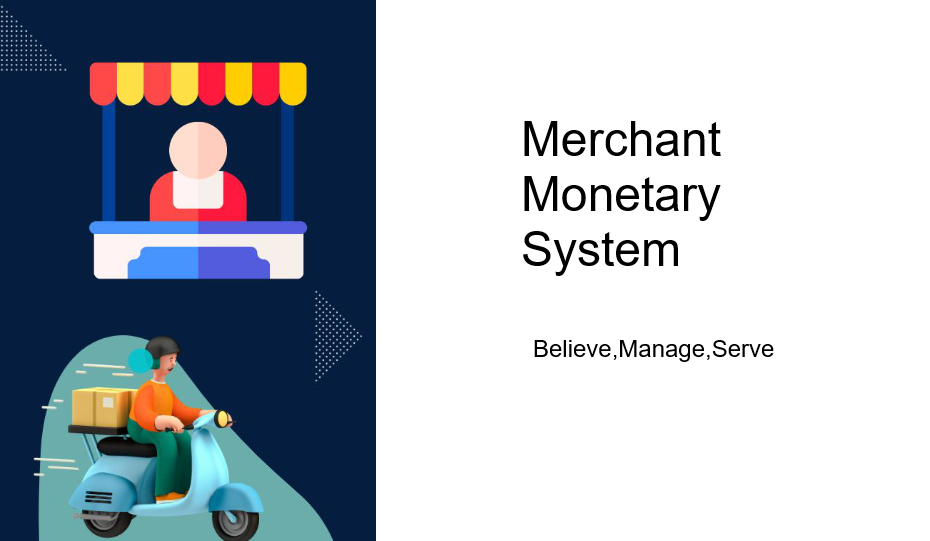
\includegraphics[scale=0.3]{./User Interface/UI-001 Intro@1x.png}\end{center}  \\ \hline

Actual Interface in Visual Studio & \begin{center} 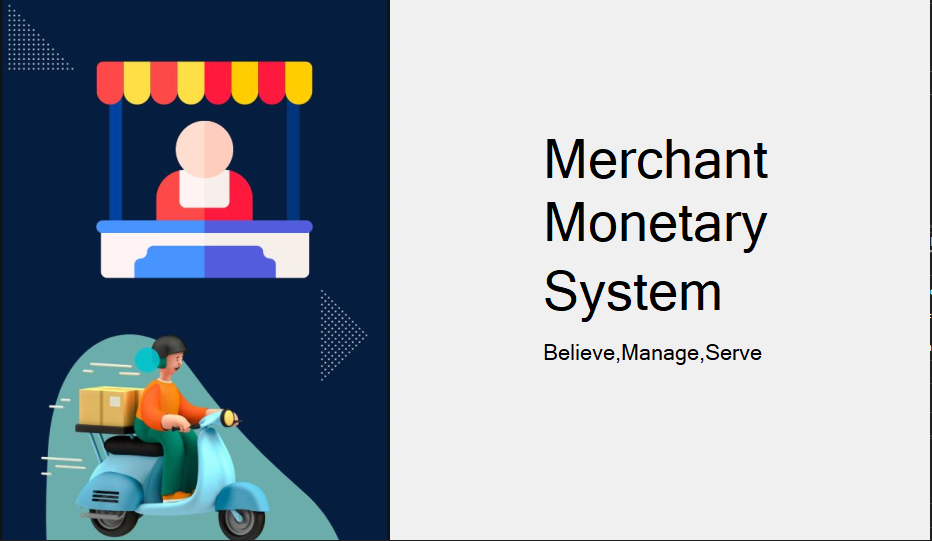
\includegraphics[scale=0.3]{./User Interface1/UI-001 Intro@1x.png}\end{center}  \\ \hline


\end{longtable}
%------------------------------------------
\subsection{Login}
\begin{longtable}{| p{3cm}|p{12cm}|}
\multicolumn{2}{c}{}
\endfirsthead
\multicolumn{2}{c}{\tablename\ \thetable\ -- \textit{Continued from previous page}}\\
\multicolumn{2}{c}{}\\
\hline
\endhead
\hline \multicolumn{2}{r}{\tablename\ \thetable\ -- \textit{Continued on next page}} \\
\endfoot
\hline
\endlastfoot
\hline

Interface ID & I02  \\\hline

Name  	      & Login  \\ \hline

Linked Use Case & U01 \\ \hline

UI Interface in JUSTINMIND & \begin{center} 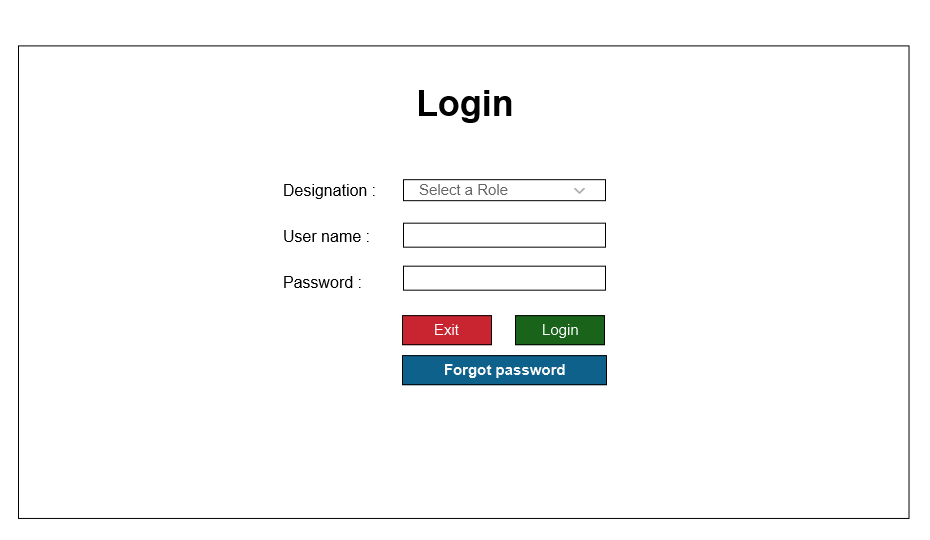
\includegraphics[scale=0.3]{./User Interface/UI-002 Login@1x.png}\end{center}  \\ \hline

Actual Interface in Visual Studio  & \begin{center} 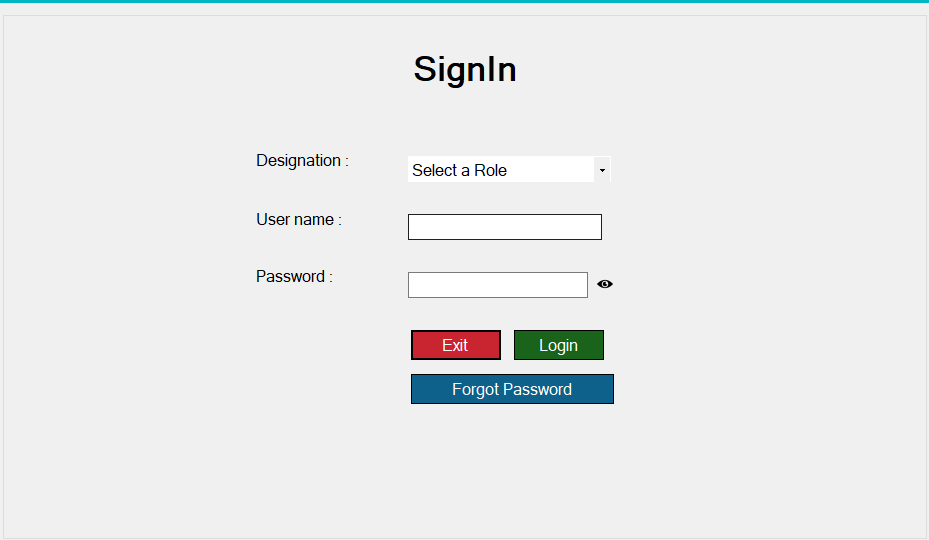
\includegraphics[scale=0.3]{./User Interface1/UI-002 Login@1x.png}\end{center}  \\ \hline

Validators & 
\begin{itemize}
\item  Username must be three character long. 
\item  Password must be eight character long.
\item All required fields must be filled correctly. 
\end{itemize}
\\ \hline

\end{longtable}
%------------------------------------------
\subsection{Forgot Password }

\begin{longtable}{| p{3cm}|p{12cm}|}
\multicolumn{2}{c}{}
\endfirsthead
\multicolumn{2}{c}{\tablename\ \thetable\ -- \textit{Continued from previous page}}\\
\multicolumn{2}{c}{}\\
\hline
\endhead
\hline \multicolumn{2}{r}{\tablename\ \thetable\ -- \textit{Continued on next page}} \\
\endfoot
\hline
\endlastfoot
\hline

Interface ID &  103 \\\hline

Name  	      & Forgot Password  \\ \hline

Linked Use Case & U02 \\ \hline

UI Interface in JUSTINMIND & \begin{center} 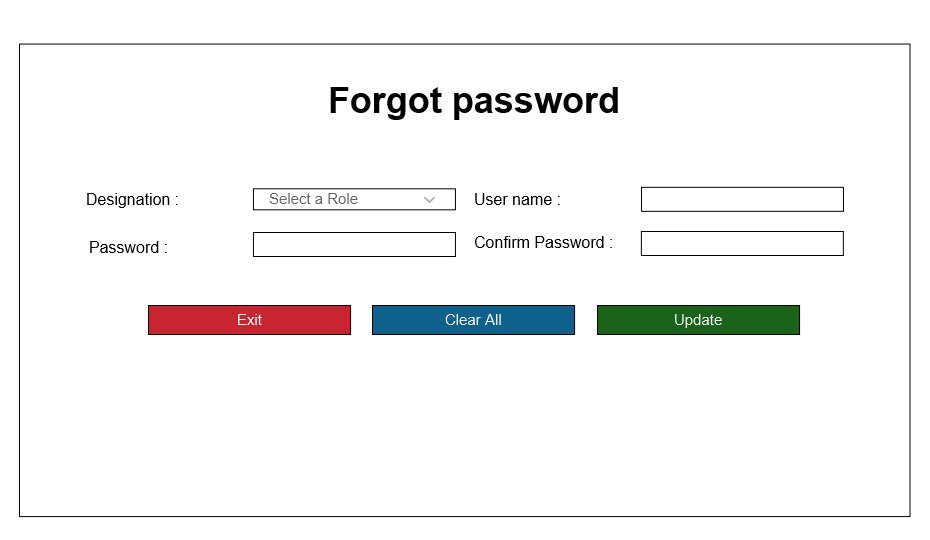
\includegraphics[scale=0.3]{./User Interface/UI-003 Forgot password@1x.png}\end{center}  \\ \hline

Actual Interface in Visual Studio  & \begin{center} 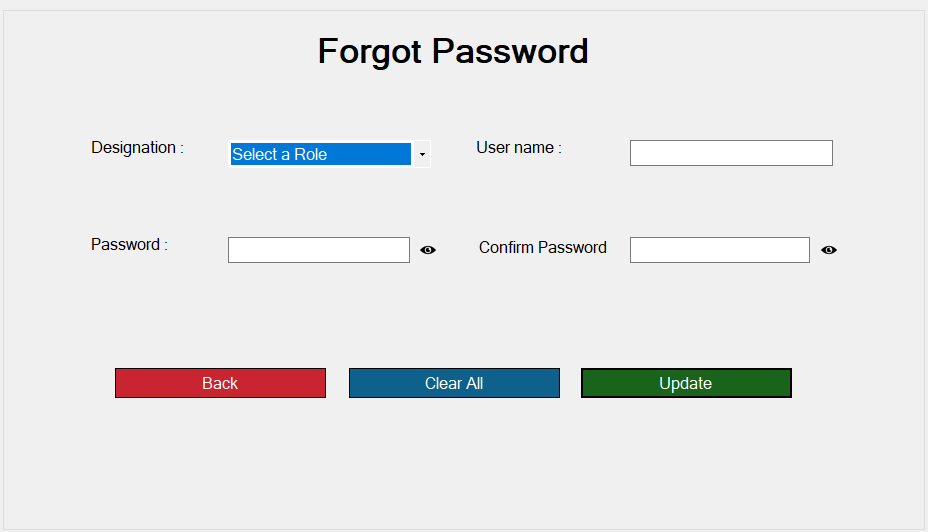
\includegraphics[scale=0.3]{./User Interface1/UI-003 Forgot password@1x.png}\end{center}  \\ \hline


Validators & 
\begin{itemize}
\item  Password should be eight character long including upper case, lower case, number and special character.
\item  Username must be exist in the system.
\item  Password and Confirm Password should be same.
\item All required fields must be filled correctly. 
\end{itemize}
\\ \hline

\end{longtable}
%------------------------------------------
\subsection{SignUp}

\begin{longtable}{| p{3cm}|p{12cm}|}
\multicolumn{2}{c}{}
\endfirsthead
\multicolumn{2}{c}{\tablename\ \thetable\ -- \textit{Continued from previous page}}\\
\multicolumn{2}{c}{}\\
\hline
\endhead
\hline \multicolumn{2}{r}{\tablename\ \thetable\ -- \textit{Continued on next page}} \\
\endfoot
\hline
\endlastfoot
\hline

Interface ID &   104 \\\hline

Name  	      &   SignUp\\ \hline

Linked Use Case &  U05\\ \hline

UI Interface in JUSTINMIND & \begin{center} 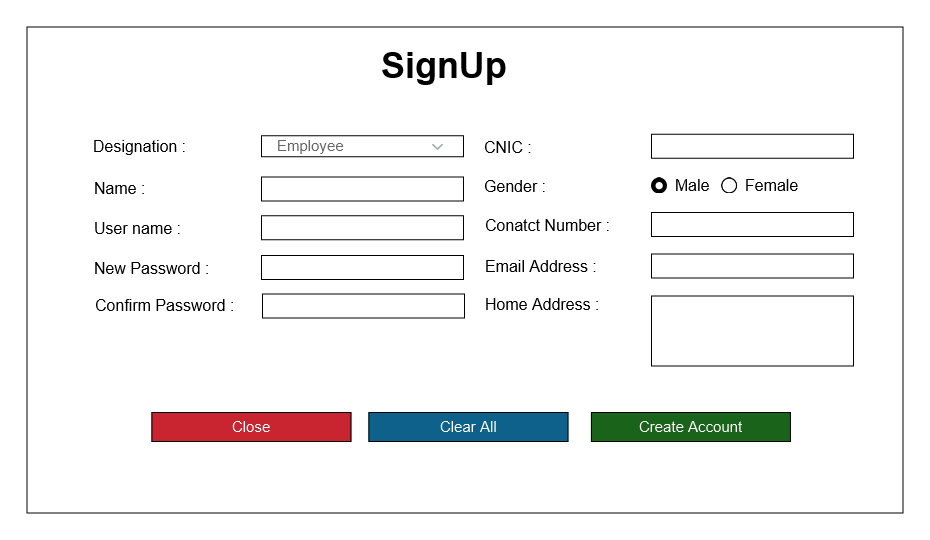
\includegraphics[scale=0.3]{./User Interface/UI-004a Create Account Except Rider@1x.png}\end{center}  \\ \hline


Actual Interface in Visual Studio & \begin{center} 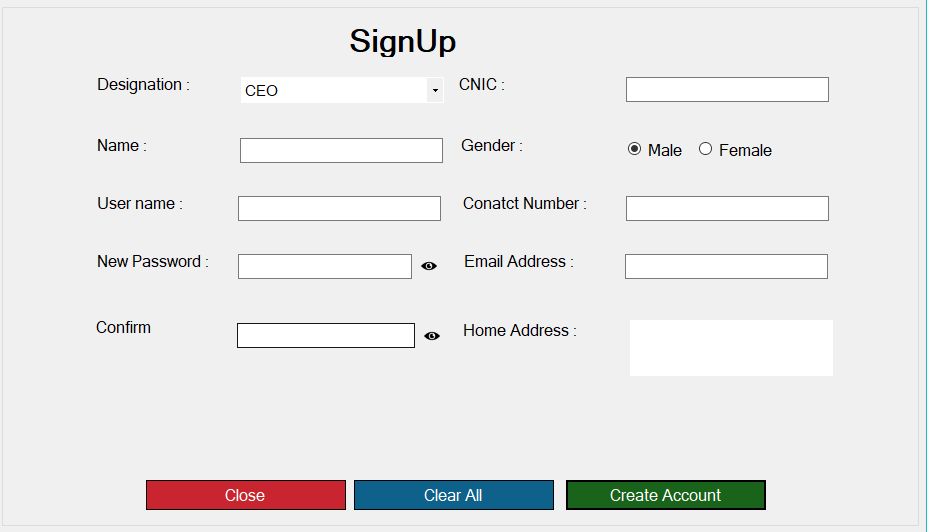
\includegraphics[scale=0.3]{./User Interface1/UI-004a Create Account Except Rider@1x.png}\end{center}  \\ \hline

Validators & 
\begin{itemize}
\item  The name should be the alphabet.
\item  Username must be three character long and enter username not matched with existing data.
\item Password should be eight character long including upper case, lower case, number and special character.

\item  Password and Confirm Password should be same.
\item  Contact number must be numeric. 
\item  CNIC must be of 13 digits.
\item  Email should include dot, at the rate symbol and correct service provider.
\item Home Address should not be empty. 
\item All required fields must be filled correctly. 
\end{itemize}
\\ \hline

\end{longtable} 
%------------------------------------------

\subsection{Update Account Information (CEO)}

\begin{longtable}{| p{3cm}|p{12cm}|}
\multicolumn{2}{c}{}
\endfirsthead
\multicolumn{2}{c}{\tablename\ \thetable\ -- \textit{Continued from previous page}}\\
\multicolumn{2}{c}{}\\
\hline
\endhead
\hline \multicolumn{2}{r}{\tablename\ \thetable\ -- \textit{Continued on next page}} \\
\endfoot
\hline
\endlastfoot
\hline

Interface ID &  I05 \\\hline

Name  	      &  Update Account Information (CEO) \\ \hline

Linked Use Case & U06 \\ \hline

UI Interface in JUSTINMIND & \begin{center} 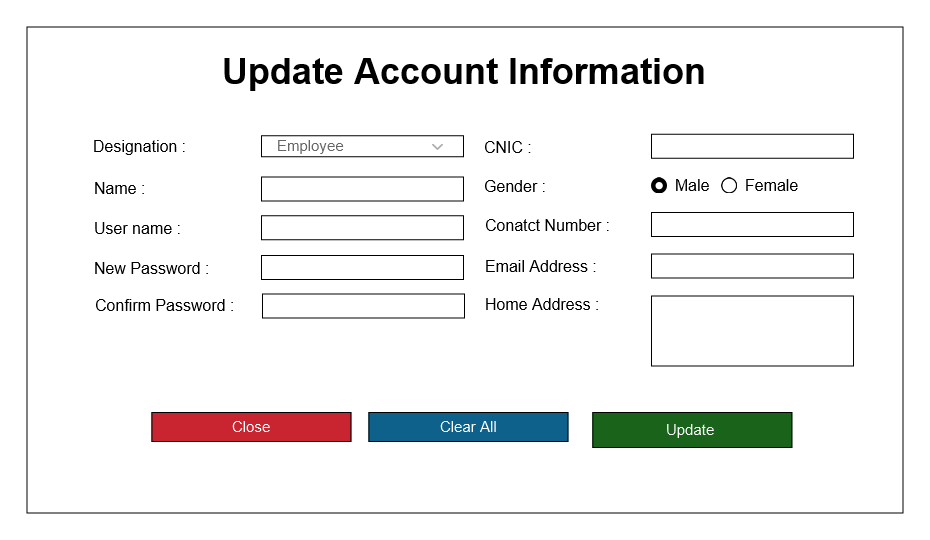
\includegraphics[scale=0.3]{./User Interface/UI-005a Update Account Information.png}\end{center}  \\ \hline

Actual Interface in Visual Studio  & \begin{center} 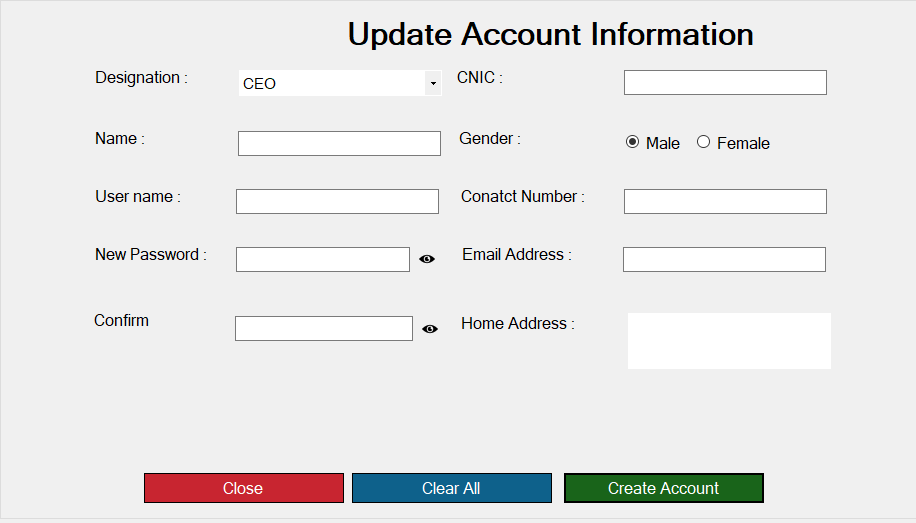
\includegraphics[scale=0.3]{./User Interface1/UI-005a Update Account Information.png}\end{center}  \\ \hline

Validators & 
\begin{itemize}
\item  The name should be the alphabet.
\item  Username must be three character long and enter username not matched with existing data.
\item Password should be eight character long including upper case, lower case, number and special character.

\item  Password and Confirm Password should be same.
\item  Contact number must be numeric. 
\item  CNIC must be of 13 digits.
\item  Email should include dot, at the rate symbol and correct service provider.
\item Home Address should not be empty. 
\item All required fields must be filled correctly. 
\end{itemize}
\\ \hline

\end{longtable} 
%------------------------------------------
%------------------------------------------

\subsection{Update Account Information (Employee)}
\begin{longtable}{| p{3cm}|p{12cm}|}
\multicolumn{2}{c}{}
\endfirsthead
\multicolumn{2}{c}{\tablename\ \thetable\ -- \textit{Continued from previous page}}\\
\multicolumn{2}{c}{}\\
\hline
\endhead
\hline \multicolumn{2}{r}{\tablename\ \thetable\ -- \textit{Continued on next page}} \\
\endfoot
\hline
\endlastfoot
\hline

Interface ID &  I07 \\\hline

Name  	      &  Update Account Information (Employee) \\ \hline

Linked Use Case & U04 \\ \hline

UI Interface in JUSTINMIND & \begin{center} 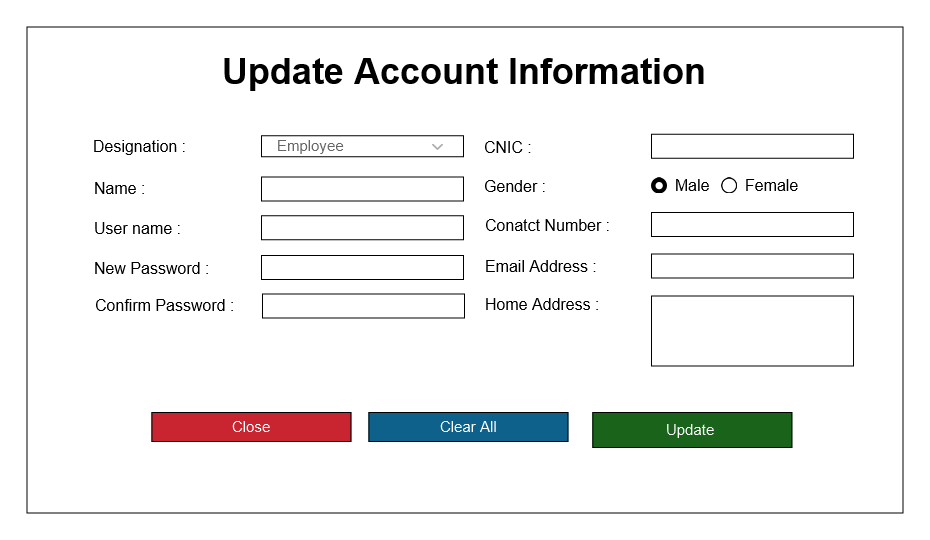
\includegraphics[scale=0.3]{./User Interface/UI-005a Update Account Information.png}\end{center}  \\ \hline

Actual Interface in Visual Studio  & \begin{center} 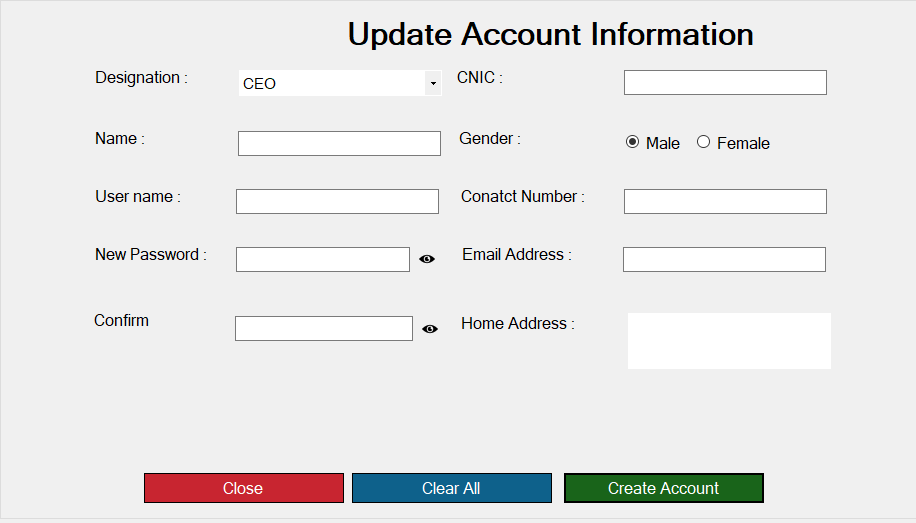
\includegraphics[scale=0.3]{./User Interface1/UI-005a Update Account Information.png}\end{center}  \\ \hline

Validators & 
\begin{itemize}
\item  The name should be the alphabet.
\item  Username must be three character long and enter username not matched with existing data.
\item Password should be eight character long including upper case, lower case, number and special character.

\item  Password and Confirm Password should be same.
\item  Contact number must be numeric. 
\item  CNIC must be of 13 digits.
\item  Email should include dot, at the rate symbol and correct service provider.
\item Home Address should not be empty. 
\item All required fields must be filled correctly. 
\end{itemize}
\\ \hline

\end{longtable} 
%------------------------------------------
\subsection{Account Detail (CEO) }

\begin{longtable}{| p{3cm}|p{12cm}|}
\multicolumn{2}{c}{}
\endfirsthead
\multicolumn{2}{c}{\tablename\ \thetable\ -- \textit{Continued from previous page}}\\
\multicolumn{2}{c}{}\\
\hline
\endhead
\hline \multicolumn{2}{r}{\tablename\ \thetable\ -- \textit{Continued on next page}} \\
\endfoot
\hline
\endlastfoot
\hline

Interface ID &  I07 \\\hline

Name  	      &  Account Detail (CEO) \\ \hline

Linked Use Case & U06 \\ \hline


UI Interface in JUSTINMIND & \begin{center} 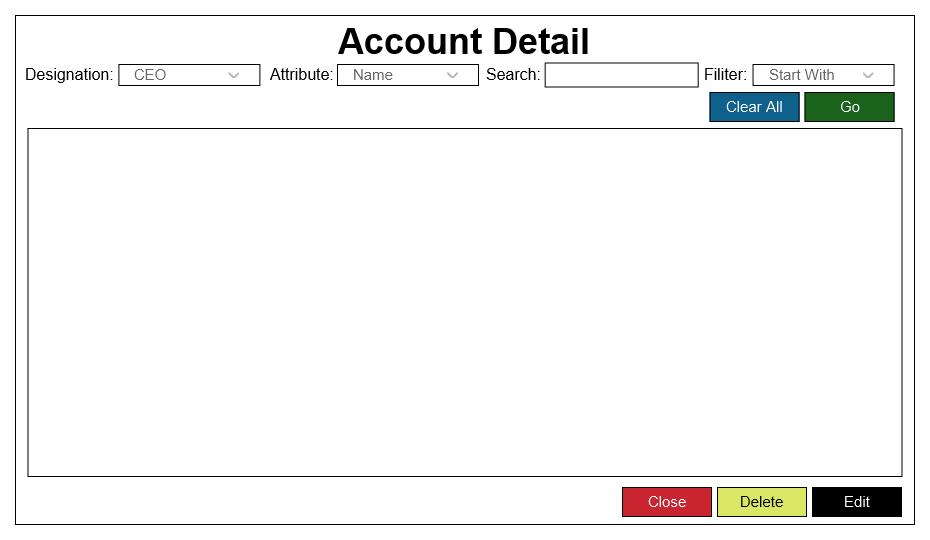
\includegraphics[scale=0.3]{./User Interface/UI-006 ViewAndDelete Account@1x.png}\end{center}  \\ \hline

Actual Interface in Visual Studio  & \begin{center} 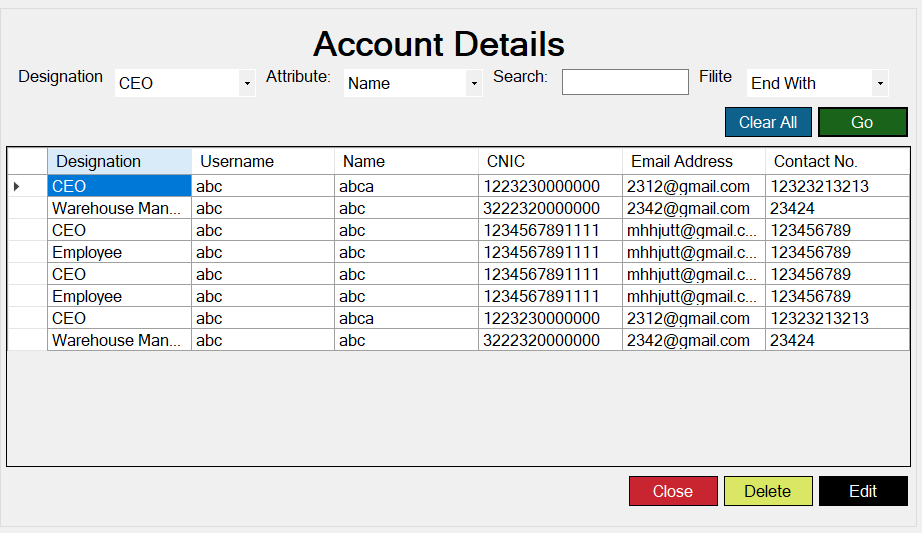
\includegraphics[scale=0.3]{./User Interface1/UI-006 ViewAndDelete Account@1x.png}\end{center}  \\ \hline

Validators & 
\begin{itemize}
\item Load button should be clicked to view data.
\item   On clicked delete and edit button there is must to select any column first from grid list. 
\item  Filters must be applied before clicking Go
\item All required fields must be filled correctly. 

\end{itemize}
\\ \hline

\end{longtable}
%------------------------------------------
%------------------------------------------
\subsection{Account Detail (Employee) }

\begin{longtable}{| p{3cm}|p{12cm}|}
\multicolumn{2}{c}{}
\endfirsthead
\multicolumn{2}{c}{\tablename\ \thetable\ -- \textit{Continued from previous page}}\\
\multicolumn{2}{c}{}\\
\hline
\endhead
\hline \multicolumn{2}{r}{\tablename\ \thetable\ -- \textit{Continued on next page}} \\
\endfoot
\hline
\endlastfoot
\hline

Interface ID &  I08 \\\hline

Name  	      &  Account Detail (Employee) \\ \hline

Linked Use Case & U07 \\ \hline


UI Interface in JUSTINMIND & \begin{center} 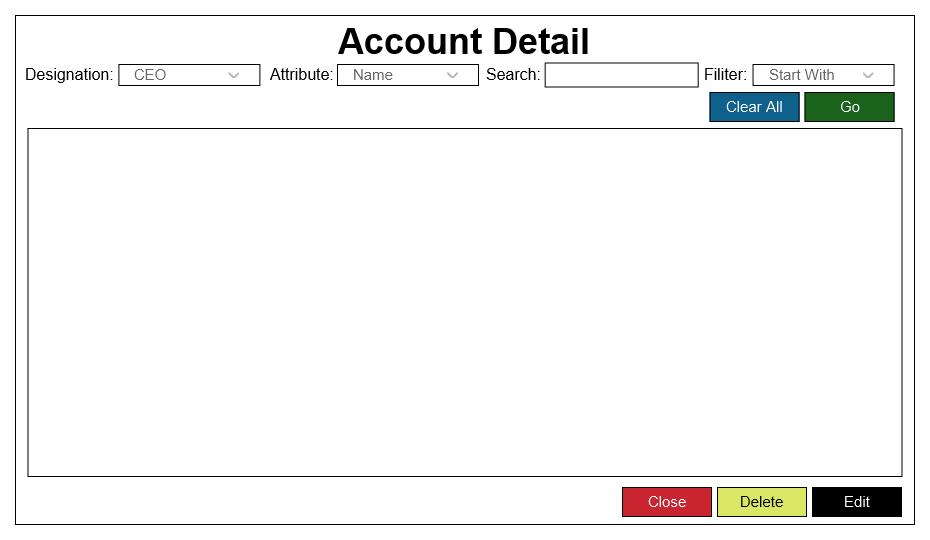
\includegraphics[scale=0.3]{./User Interface/UI-006 ViewAndDelete Account@1x.png}\end{center}  \\ \hline


Actual Interface in Visual Studio  & \begin{center} 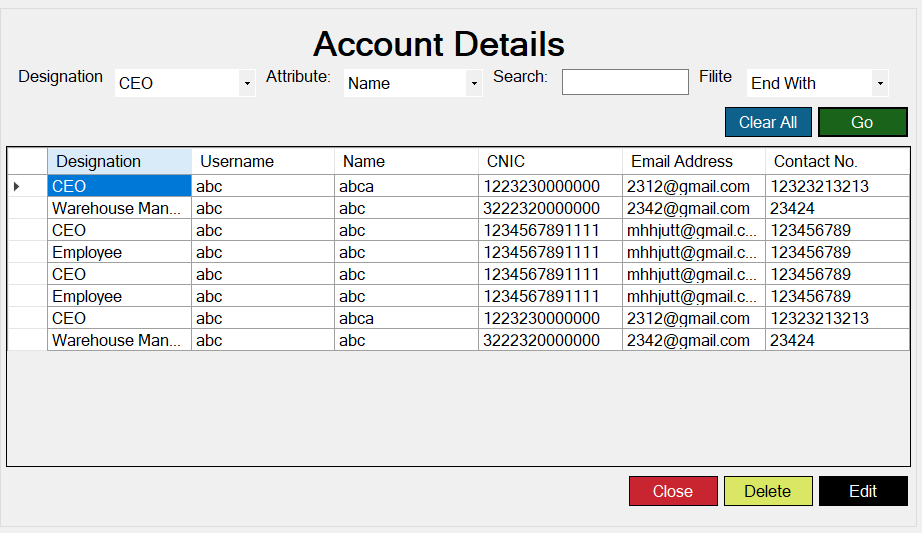
\includegraphics[scale=0.3]{./User Interface1/UI-006 ViewAndDelete Account@1x.png}\end{center}  \\ \hline

Validators & 
\begin{itemize}
\item Load button should be clicked to view data.
\item   On clicked delete and edit button there is must to select any row first from the data grid view. 
\item  Filters must be applied before clicking Go button.
\item All required fields must be filled correctly. 

\end{itemize}
\\ \hline

\end{longtable}
%------------------------------------------
\subsection{CEO Dashboard }
\begin{longtable}{| p{3cm}|p{12cm}|}
\multicolumn{2}{c}{}
\endfirsthead
\multicolumn{2}{c}{\tablename\ \thetable\ -- \textit{Continued from previous page}}\\
\multicolumn{2}{c}{}\\
\hline
\endhead
\hline \multicolumn{2}{r}{\tablename\ \thetable\ -- \textit{Continued on next page}} \\
\endfoot
\hline
\endlastfoot
\hline

Interface ID &  I09 \\\hline

Name  	      & CEO Dashboard  \\ \hline

UI Interface in JUSTINMIND & \begin{center} 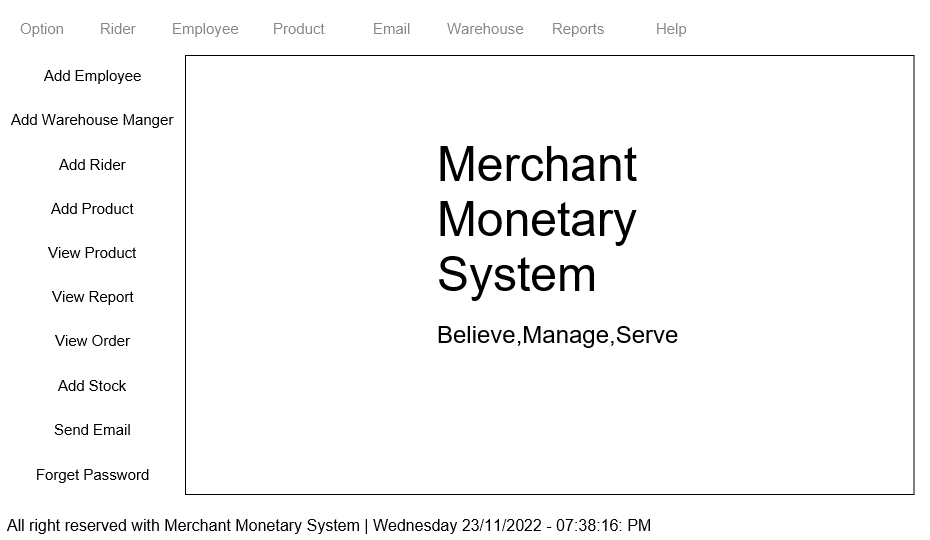
\includegraphics[scale=0.3]{./User Interface/UI-007 CEO Dashboard@1x.png}\end{center}  \\ \hline

Actual Interface in Visual Studio  & \begin{center} 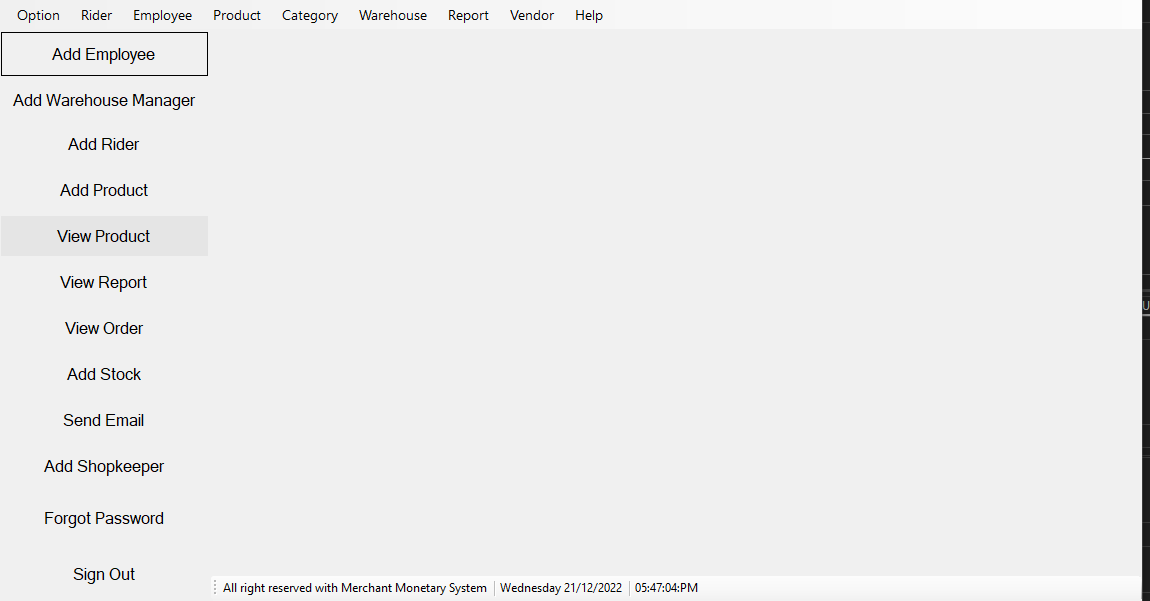
\includegraphics[scale=0.3]{./User Interface1/UI-007 CEO Dashboard@1x.png}\end{center}  \\ \hline

\end{longtable}
%------------------------------------------
\subsection{Add Product }

\begin{longtable}{| p{3cm}|p{12cm}|}
\multicolumn{2}{c}{}
\endfirsthead
\multicolumn{2}{c}{\tablename\ \thetable\ -- \textit{Continued from previous page}}\\
\multicolumn{2}{c}{}\\
\hline
\endhead
\hline \multicolumn{2}{r}{\tablename\ \thetable\ -- \textit{Continued on next page}} \\
\endfoot
\hline
\endlastfoot
\hline

Interface ID & I10  \\\hline

Name & Add Product  \\ \hline

Linked Use Case & U08	 \\ \hline


UI Interface in JUSTINMIND & \begin{center} 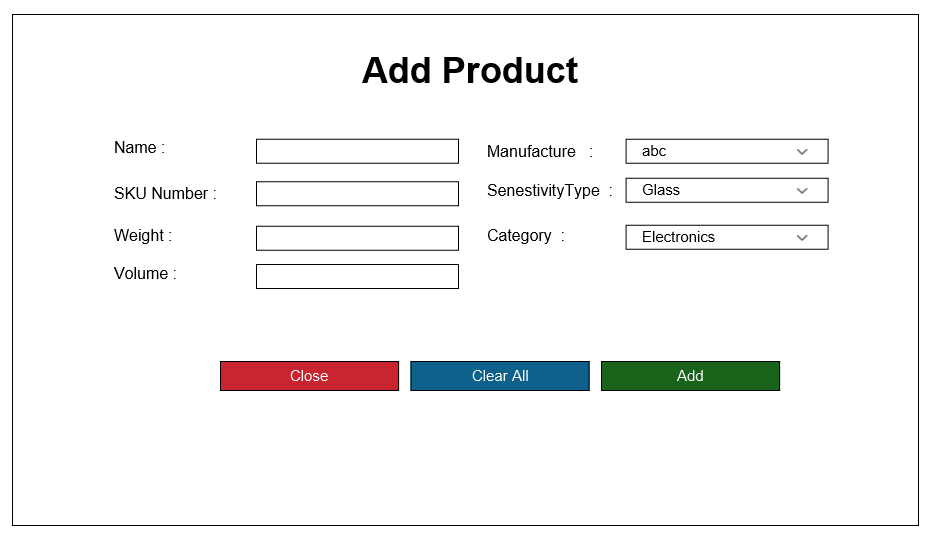
\includegraphics[scale=0.3]{./User Interface/UI-008 Add Product@1x.png}\end{center}  \\ \hline


Actual Interface in Visual Studio  & \begin{center} 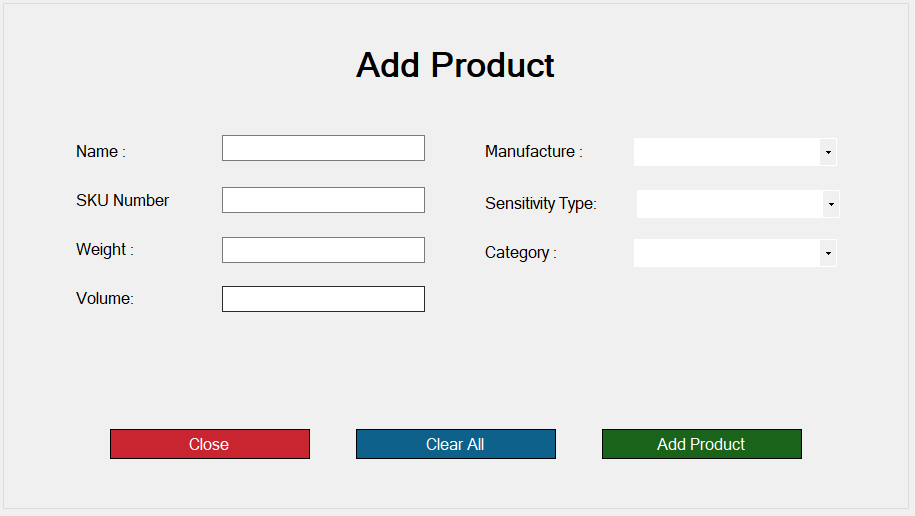
\includegraphics[scale=0.3]{./User Interface1/UI-008 Add Product@1x.png}\end{center}  \\ \hline

Validators & 
\begin{itemize}
\item Name must contain only digits and alphabets.
\item SKU-ID must be number.
\item Weight and Volume must be in integers or float and positive.
\item All required fields must be filled correctly. 

\end{itemize}
\\ \hline

\end{longtable}
%------------------------------------------
\subsection{Update Product Record}

\begin{longtable}{| p{3cm}|p{12cm}|}
\multicolumn{2}{c}{}
\endfirsthead
\multicolumn{2}{c}{\tablename\ \thetable\ -- \textit{Continued from previous page}}\\
\multicolumn{2}{c}{}\\
\hline
\endhead
\hline \multicolumn{2}{r}{\tablename\ \thetable\ -- \textit{Continued on next page}} \\
\endfoot
\hline
\endlastfoot
\hline

Interface ID & I11  \\\hline

Name  &  Update Product Record \\ \hline

Linked Use Case & U09	  \\ \hline


UI Interface in JUSTINMIND & \begin{center} 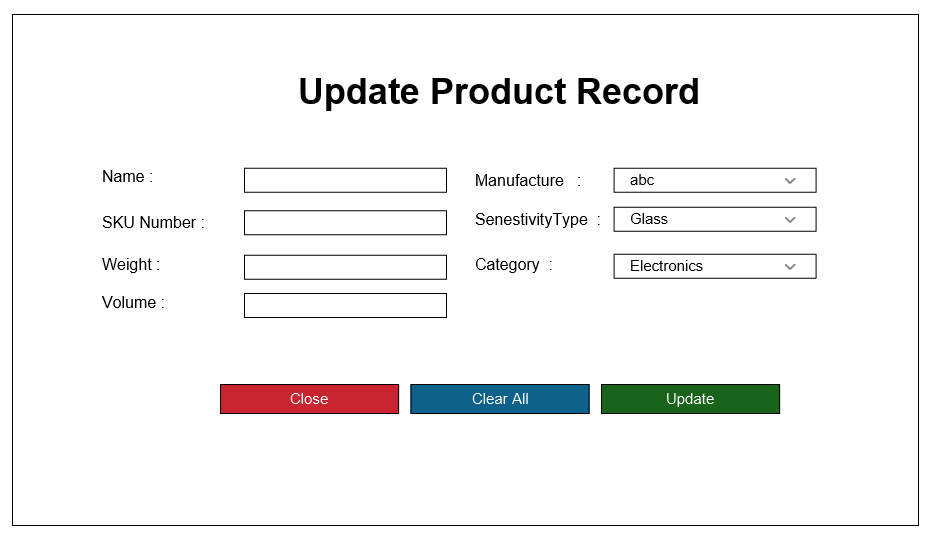
\includegraphics[scale=0.3]{./User Interface/UI-009 Update Product Record@1x.png}\end{center}  \\ \hline


Actual Interface in Visual Studio  & \begin{center} 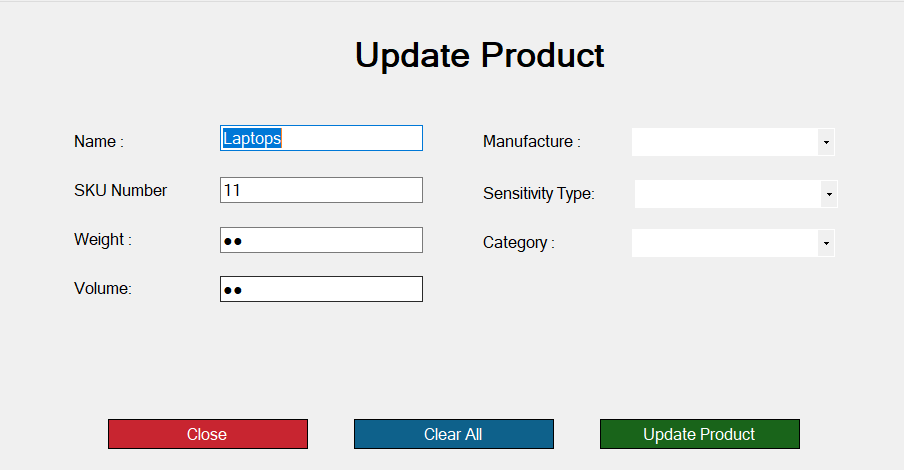
\includegraphics[scale=0.3]{./User Interface1/UI-009 Update Product Record@1x.png}\end{center}  \\ \hline

Validators & 
\begin{itemize}
\item Name must contain only digits and alphabets.
\item SKU-ID must be number.
\item Weight and Volume must be in integers or float and positive.\item All required fields must be filled correctly. 
\end{itemize}
\\ \hline

\end{longtable} 
%------------------------------------------
%------------------------------------------
\subsection{Take Order}

\begin{longtable}{| p{3cm}|p{12cm}|}
\multicolumn{2}{c}{}
\endfirsthead
\multicolumn{2}{c}{\tablename\ \thetable\ -- \textit{Continued from previous page}}\\
\multicolumn{2}{c}{}\\
\hline
\endhead
\hline \multicolumn{2}{r}{\tablename\ \thetable\ -- \textit{Continued on next page}} \\
\endfoot
\hline
\endlastfoot
\hline

Interface ID & I12 \\\hline

Name  &  Take Order \\ \hline

Linked Use Case & U19	 \\ \hline

UI Interface in JUSTINMIND & \begin{center} 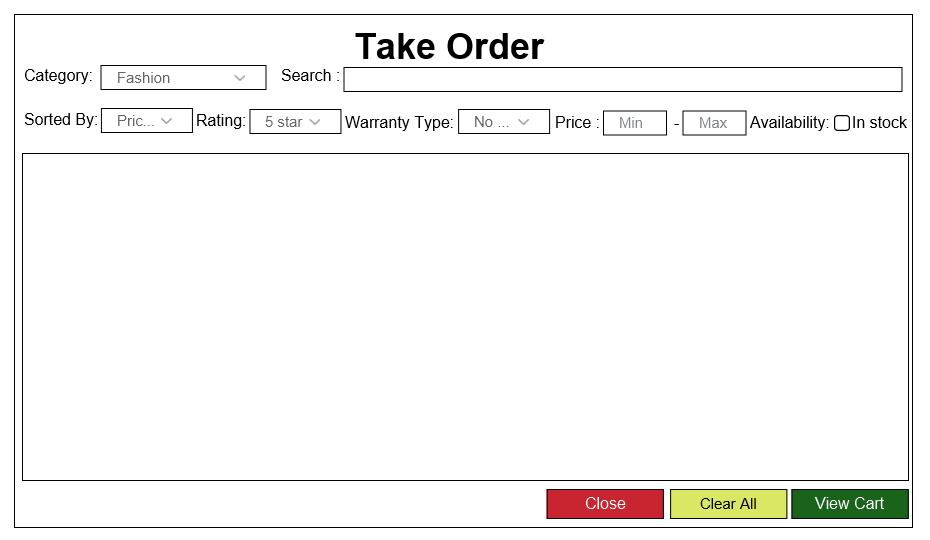
\includegraphics[scale=0.3]{./User Interface/UI-011 Order Product@1x.png}\end{center}  \\ \hline

Actual Interface in Visual Studio  & \begin{center} 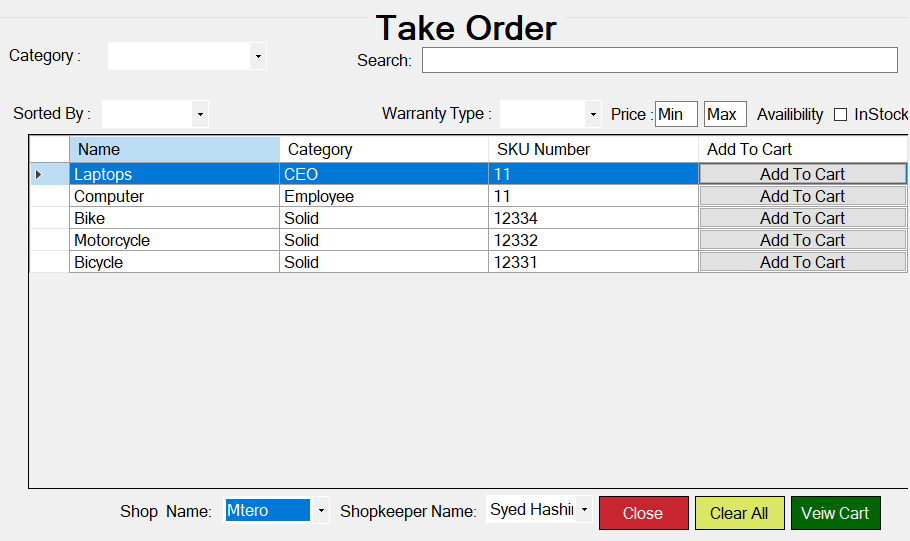
\includegraphics[scale=0.3]{./User Interface1/UI-011 Order Product@1x.png}\end{center}  \\ \hline

Validators & 
\begin{itemize}
\item   
Price must be positive integer or float.
\item 
Search text only contains alphabets and integers only.
\item All required fields must be filled correctly. 
\end{itemize}
\\ \hline

\end{longtable}
%------------------------------------------
%------------------------------------------
\subsection{Email }

\begin{longtable}{| p{3cm}|p{12cm}|}
\multicolumn{2}{c}{}
\endfirsthead
\multicolumn{2}{c}{\tablename\ \thetable\ -- \textit{Continued from previous page}}\\
\multicolumn{2}{c}{}\\
\hline
\endhead
\hline \multicolumn{2}{r}{\tablename\ \thetable\ -- \textit{Continued on next page}} \\
\endfoot
\hline
\endlastfoot
\hline

Interface ID & I13  \\\hline

Name  & Email \\ \hline

Linked Use Case & U37	 \\ \hline

UI Interface in JUSTINMIND & \begin{center} \includegraphics[scale=0.3]{./User Interface/UI-012 SendEmail@1x.png}\end{center}  \\ \hline

Actual Interface in Visual Studio & \begin{center} \includegraphics[scale=0.3]{./User Interface1/UI-012 SendEmail@1x.png}\end{center}  \\ \hline

Validators & 
\begin{itemize}
\item  To section must be filled to send the mail.
\item All required fields must be filled correctly. 


\end{itemize}
\\ \hline

\end{longtable} 
%------------------------------------------
\subsection{Add Warehouse}
\begin{longtable}{| p{3cm}|p{12cm}|}
\multicolumn{2}{c}{}
\endfirsthead
\multicolumn{2}{c}{\tablename\ \thetable\ -- \textit{Continued from previous page}}\\
\multicolumn{2}{c}{}\\
\hline
\endhead
\hline \multicolumn{2}{r}{\tablename\ \thetable\ -- \textit{Continued on next page}} \\
\endfoot
\hline
\endlastfoot
\hline

Interface ID &  I14 \\\hline

Name  & Add Warehouse  \\ \hline

Linked Use Case & U16	 \\ \hline


UI Interface in JUSTINMIND & \begin{center} \includegraphics[scale=0.3]{./User Interface/UI-013 AddWarehouse@1x.png}\end{center}  \\ \hline


Actual Interface in Visual Studio  & \begin{center} \includegraphics[scale=0.3]{./User Interface1/UI-013 AddWarehouse@1x.png}\end{center}  \\ \hline


Validators & 
\begin{itemize}
\item Name must contain only digits and alphabets.
\item Capacity in volume must be in integers or float and positive.
\item All required fields must be filled correctly. 
\end{itemize}
\\ \hline

\end{longtable}
%------------------------------------------
\subsection{Update Warehouse Record}

\begin{longtable}{| p{3cm}|p{12cm}|}
\multicolumn{2}{c}{}
\endfirsthead
\multicolumn{2}{c}{\tablename\ \thetable\ -- \textit{Continued from previous page}}\\
\multicolumn{2}{c}{}\\
\hline
\endhead
\hline \multicolumn{2}{r}{\tablename\ \thetable\ -- \textit{Continued on next page}} \\
\endfoot
\hline
\endlastfoot
\hline

Interface ID & I15  \\\hline

Name  &  Update Warehouse Record \\ \hline

Linked Use Case & U17 \\ \hline

UI Interface in JUSTINMIND & \begin{center} 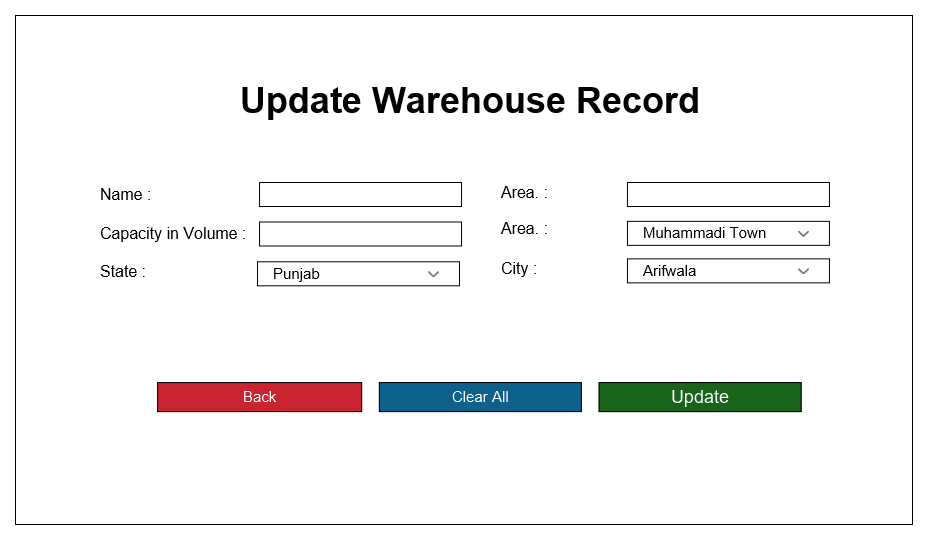
\includegraphics[scale=0.3]{./User Interface/UI-014 EditWarehouse@1x.png}\end{center}  \\ \hline

Actual Interface in Visual Studio  & \begin{center} 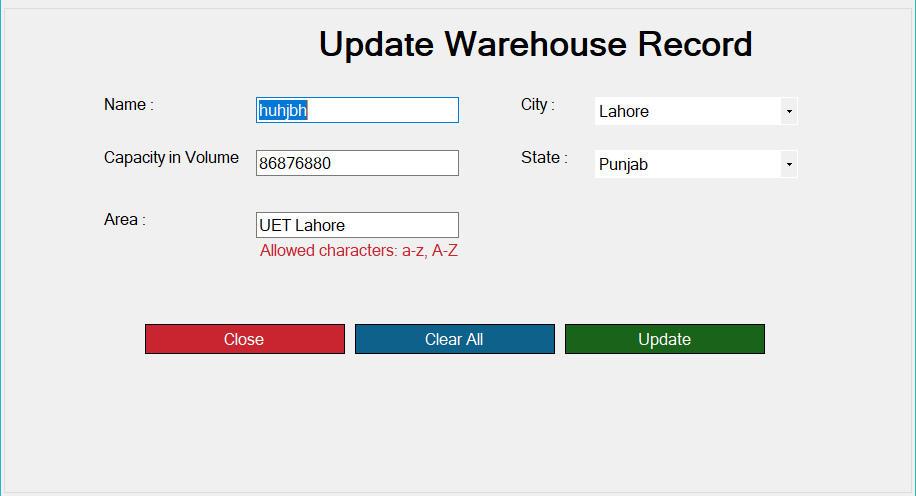
\includegraphics[scale=0.3]{./User Interface1/UI-014 EditWarehouse@1x.png}\end{center}  \\ \hline

Validators & 
\begin{itemize}
\item   Space fields and Street No. input must be a number
\item  Necessary fields must be filled before updating


\end{itemize}
\\ \hline

\end{longtable}
%------------------------------------------
\subsection{Warehouse Detail }

\begin{longtable}{| p{3cm}|p{12cm}|}
\multicolumn{2}{c}{}
\endfirsthead
\multicolumn{2}{c}{\tablename\ \thetable\ -- \textit{Continued from previous page}}\\
\multicolumn{2}{c}{}\\
\hline
\endhead
\hline \multicolumn{2}{r}{\tablename\ \thetable\ -- \textit{Continued on next page}} \\
\endfoot
\hline
\endlastfoot
\hline

Interface ID & I16  \\\hline

Name  &  Warehouse Detail \\ \hline

Linked Use Case & U18 \\ \hline

UI Interface in JUSTINMIND & \begin{center} \includegraphics[scale=0.3]{./User Interface/UI-015 ViewAndDelete Warehouse@.png}\end{center}  \\ \hline


Actual Interface in Visual Studio  & \begin{center} \includegraphics[scale=0.3]{./User Interface1/UI-015 ViewAndDelete Warehouse@.png}\end{center}  \\ \hline

Validators & 
\begin{itemize}
\item Load button should be clicked to view data.
\item Name must contain only digits and alphabets.
\item Capacity in volume must be in integers or float and positive.
\item All required fields must be filled correctly. 
\end{itemize}
\\ \hline

\end{longtable} 
%------------------------------------------
\subsection{Warehouse Manager Dashboard }
\begin{longtable}{| p{3cm}|p{12cm}|}
\multicolumn{2}{c}{}
\endfirsthead
\multicolumn{2}{c}{\tablename\ \thetable\ -- \textit{Continued from previous page}}\\
\multicolumn{2}{c}{}\\
\hline
\endhead
\hline \multicolumn{2}{r}{\tablename\ \thetable\ -- \textit{Continued on next page}} \\
\endfoot
\hline
\endlastfoot
\hline

Interface ID &  I17 \\\hline

Name  &  Warehouse Manager Dashboard \\ \hline

Linked Use Case & NILL \\ \hline

UI Interface in JUSTINMIND & \begin{center} 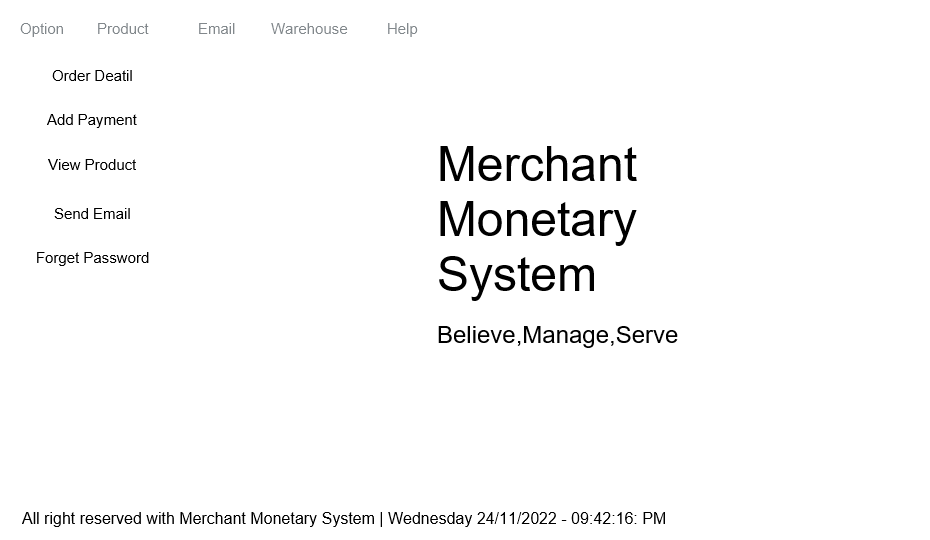
\includegraphics[scale=0.3]{./User Interface/UI-016 Warehouse Manager Dashboard@1x.png}\end{center}  \\ \hline


Actual Interface in Visual Studio  & \begin{center} 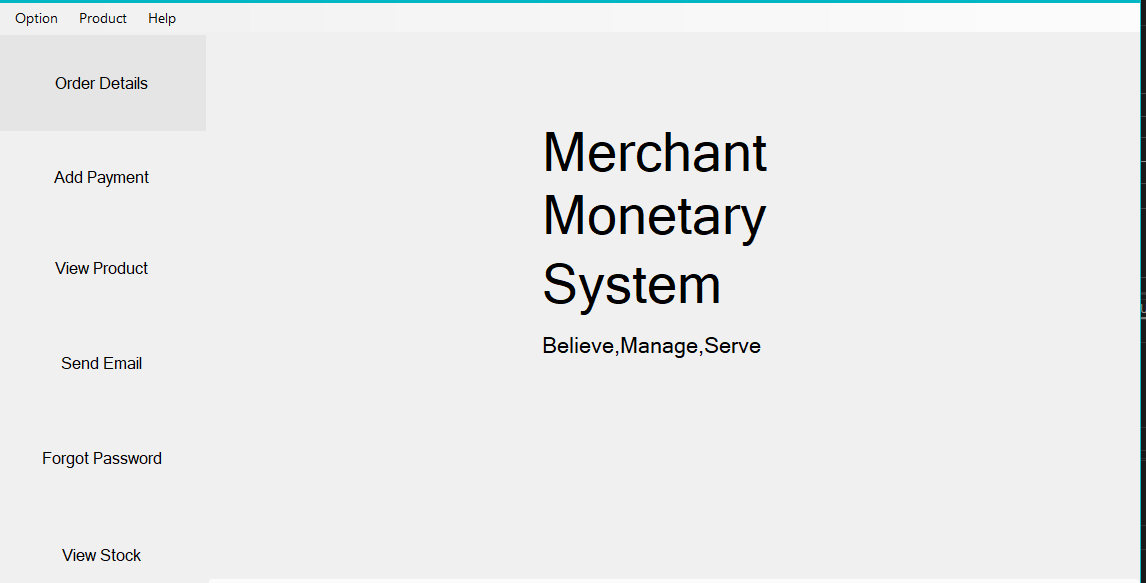
\includegraphics[scale=0.3]{./User Interface1/UI-016 Warehouse Manager Dashboard@1x.png}\end{center}  \\ \hline


\end{longtable}
%------------------------------------------
\subsection{Employee Dashboard }
\begin{longtable}{| p{3cm}|p{12cm}|}
\multicolumn{2}{c}{}
\endfirsthead
\multicolumn{2}{c}{\tablename\ \thetable\ -- \textit{Continued from previous page}}\\
\multicolumn{2}{c}{}\\
\hline
\endhead
\hline \multicolumn{2}{r}{\tablename\ \thetable\ -- \textit{Continued on next page}} \\
\endfoot
\hline
\endlastfoot
\hline

Interface ID & I18  \\\hline

Name  &  Employee Dashboard \\ \hline

Linked Use Case &  NILL \\ \hline

UI Interface in JUSTINMIND & \begin{center} 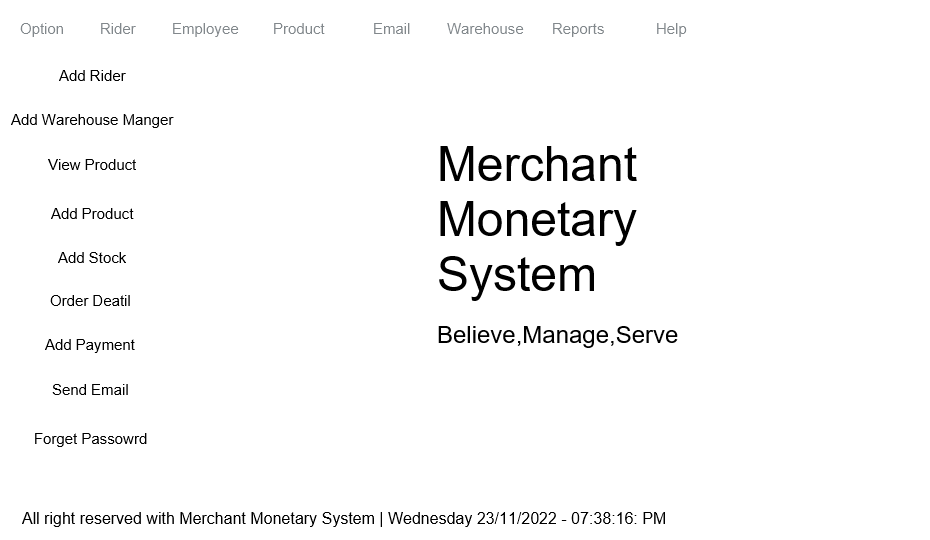
\includegraphics[scale=0.3]{./User Interface/UI-017 Employee Dashboard@1x.png}\end{center}  \\ \hline


Actual Interface in Visual Studio  & \begin{center} 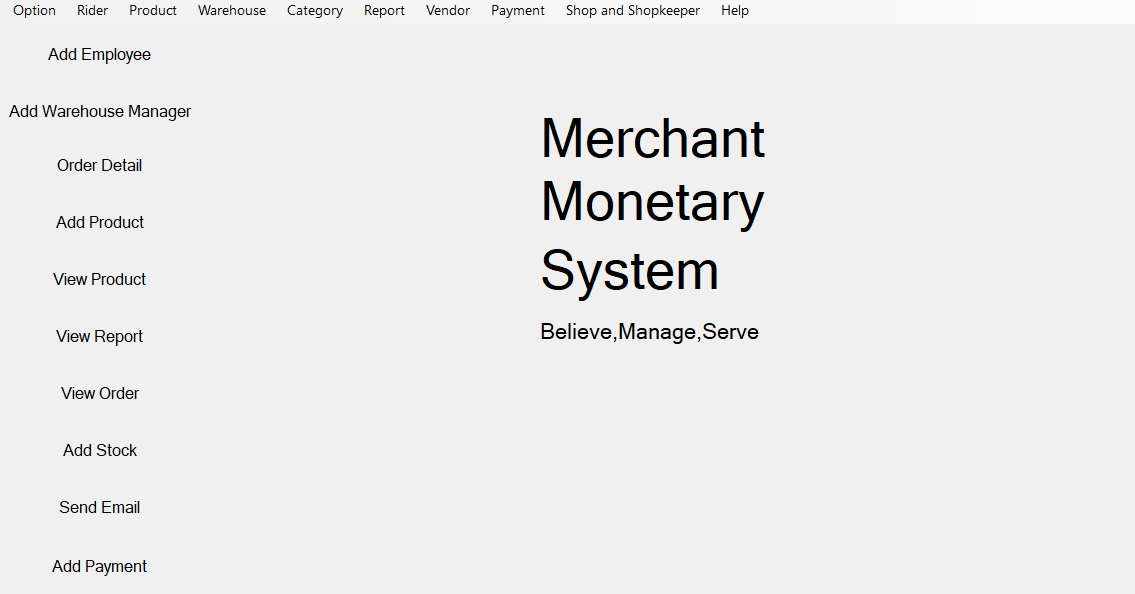
\includegraphics[scale=0.3]{./User Interface1/UI-017 Employee Dashboard@1x.png}\end{center}  \\ \hline

\end{longtable}
%------------------------------------------
\subsection{Rider Dashboard }

\begin{longtable}{| p{3cm}|p{12cm}|}
\multicolumn{2}{c}{}
\endfirsthead
\multicolumn{2}{c}{\tablename\ \thetable\ -- \textit{Continued from previous page}}\\
\multicolumn{2}{c}{}\\
\hline
\endhead
\hline \multicolumn{2}{r}{\tablename\ \thetable\ -- \textit{Continued on next page}} \\
\endfoot
\hline
\endlastfoot
\hline

Interface ID & I19  \\\hline

Name  & Rider Dashboard  \\ \hline

Linked Use Case & NILL  \\ \hline

UI Interface in JUSTINMIND & \begin{center} \includegraphics[scale=0.3]{./User Interface/UI-018 Rider Dashboard@1x.png}\end{center}  \\ \hline

Actual Interface in Visual Studio & \begin{center} \includegraphics[scale=0.3]{./User Interface1/UI-018 Rider Dashboard@1x.png}\end{center}  \\ \hline

\end{longtable}
%------------------------------------------

%------------------------------------------
\subsection{View Route }

\begin{longtable}{| p{3cm}|p{12cm}|}
\multicolumn{2}{c}{}
\endfirsthead
\multicolumn{2}{c}{\tablename\ \thetable\ -- \textit{Continued from previous page}}\\
\multicolumn{2}{c}{}\\
\hline
\endhead
\hline \multicolumn{2}{r}{\tablename\ \thetable\ -- \textit{Continued on next page}} \\
\endfoot
\hline
\endlastfoot
\hline

Interface ID & I20  \\\hline

Name  & View Route  \\ \hline

Linked Use Case & U29  \\ \hline

UI Interface in JUSTINMIND & \begin{center} \includegraphics[scale=0.3]{./User Interface/UI-034 Route Finder@1x.png}\end{center}  \\ \hline


Actual Interface in Visual Studio  & \begin{center} \includegraphics[scale=0.3]{./User Interface1/UI-034 Route Finder@1x.png}\end{center}  \\ \hline

Validators & 
\begin{itemize}
\item  Street No. Must not be negative
\item All fields must be appropriately filled to find the routes
 \end{itemize}
 \\ \hline
\end{longtable}
%------------------------------------------

%------------------------------------------
\subsection{Add Shop/Shopkeeper}

\begin{longtable}{| p{3cm}|p{12cm}|}
\multicolumn{2}{c}{}
\endfirsthead
\multicolumn{2}{c}{\tablename\ \thetable\ -- \textit{Continued from previous page}}\\
\multicolumn{2}{c}{}\\
\hline
\endhead
\hline \multicolumn{2}{r}{\tablename\ \thetable\ -- \textit{Continued on next page}} \\
\endfoot
\hline
\endlastfoot
\hline

Interface ID &  I21 \\\hline

Name  & Add Shop/Shopkeeper \\ \hline

Linked Use Case & U23 \\ \hline

UI Interface in JUSTINMIND & \begin{center} \includegraphics[scale=0.3]{./User Interface/UI-019 Add ShopAndShopKeeper@1x.png}\end{center}  \\ \hline


Actual Interface in Visual Studio  & \begin{center} \includegraphics[scale=0.3]{./User Interface1/UI-019 Add ShopAndShopKeeper@1x.png}\end{center}  \\ \hline

Validators & 
\begin{itemize}
\item  The name should be the alphabet.
\item  Contact number must be numeric. 
\item  Email should include dot, at the rate symbol and correct service provider.
\item Home Address should not be empty. 
 
\item All required fields must be filled correctly. 
\end{itemize}
\\ \hline

\end{longtable}
%------------------------------------------
\subsection{Add Payment }

\begin{longtable}{| p{3cm}|p{12cm}|}
\multicolumn{2}{c}{}
\endfirsthead
\multicolumn{2}{c}{\tablename\ \thetable\ -- \textit{Continued from previous page}}\\
\multicolumn{2}{c}{}\\
\hline
\endhead
\hline \multicolumn{2}{r}{\tablename\ \thetable\ -- \textit{Continued on next page}} \\
\endfoot
\hline
\endlastfoot
\hline

Interface ID & I22  \\\hline

Name  &  Add Payment \\ \hline

Linked Use Case & U25	 \\ \hline

UI Interface in JUSTINMIND & \begin{center} 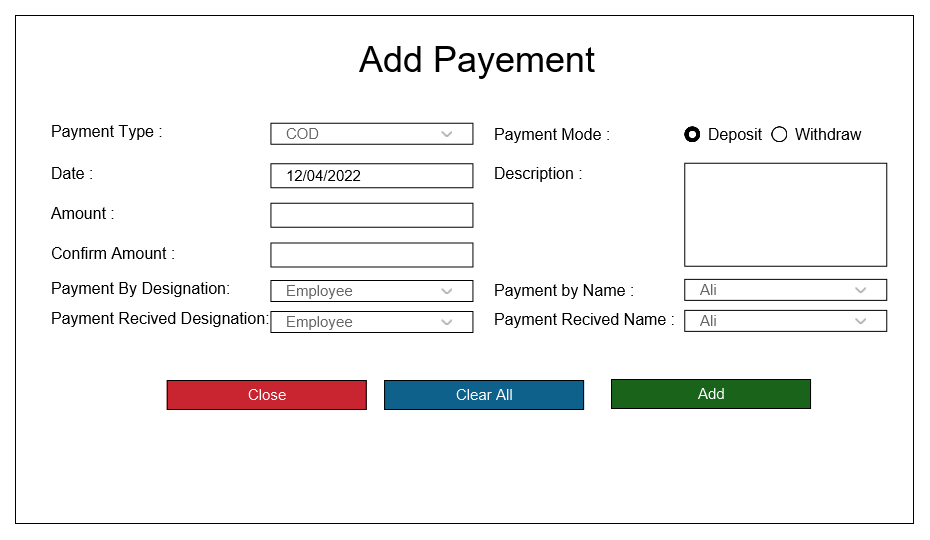
\includegraphics[scale=0.3]{./User Interface/UI-021 Add Payment@1x.png}\end{center}  \\ \hline


Actual Interface in Visual Studio  & \begin{center} 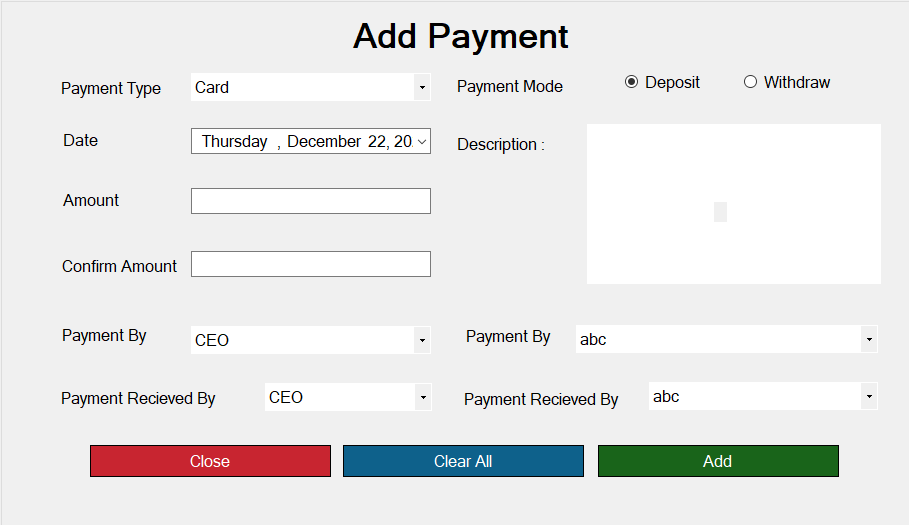
\includegraphics[scale=0.3]{./User Interface1/UI-021 Add Payment@1x.png}\end{center}  \\ \hline

Validators & 
\begin{itemize}
\item  Amount must be numeric or float.
\item Confirm amount must be matched with first typed amount.
\item Description should be entered.
\item All required fields must be filled correctly. 

\end{itemize}
\\ \hline

\end{longtable} 
%----------------------------------------
\subsection{Update Payment Information}
\begin{longtable}{| p{3cm}|p{12cm}|}
\multicolumn{2}{c}{}
\endfirsthead
\multicolumn{2}{c}{\tablename\ \thetable\ -- \textit{Continued from previous page}}\\
\multicolumn{2}{c}{}\\
\hline
\endhead
\hline \multicolumn{2}{r}{\tablename\ \thetable\ -- \textit{Continued on next page}} \\
\endfoot
\hline
\endlastfoot
\hline

Interface ID & I23  \\\hline

Name  &  Update Payment Information \\ \hline

Linked Use Case & U26	 \\ \hline

UI Interface in JUSTINMIND & \begin{center} \includegraphics[scale=0.3]{./User Interface/UI-022Update Payment Information.png}\end{center}  \\ \hline


Actual Interface in Visual Studio  & \begin{center} \includegraphics[scale=0.3]{./User Interface1/UI-022Update Payment Information.png}\end{center}  \\ \hline

Validators & 
\begin{itemize}
\item  Amount must be numeric or float.
\item Confirm amount must be matched with first typed amount.
\item Description should be entered.
\item All required fields must be filled correctly. 
\end{itemize}
\\ \hline
\end{longtable}
%------------------------------------------
\subsection{Add Vehicle}
\begin{longtable}{| p{3cm}|p{12cm}|}
\multicolumn{2}{c}{}
\endfirsthead
\multicolumn{2}{c}{\tablename\ \thetable\ -- \textit{Continued from previous page}}\\
\multicolumn{2}{c}{}\\
\hline
\endhead
\hline \multicolumn{2}{r}{\tablename\ \thetable\ -- \textit{Continued on next page}} \\
\endfoot
\hline
\endlastfoot
\hline

Interface ID & I24  \\\hline

Name  &  Add Vehicle \\ \hline

Linked Use Case & U21	 \\ \hline

UI Interface in JUSTINMIND & \begin{center} \includegraphics[scale=0.3]{./User Interface/UI-023 AddVehicle@1x.png}\end{center}  \\ \hline
Actual Interface in Visual Studio  & \begin{center} \includegraphics[scale=0.3]{./User Interface1/UI-023 AddVehicle@1x.png}\end{center}  \\ \hline

Validators & 
\begin{itemize}
\item   Registration number should contain alphabets and digits.
\item  Capacity in volume should be be numeric and positive. 
\item Capacity in weight should be be numeric and positive. 
\item All required fields must be filled correctly. 

\end{itemize}
\\ \hline
\end{longtable}
%------------------------------------------
\subsection{Update Vehicle Information}
\begin{longtable}{| p{3cm}|p{12cm}|}
\multicolumn{2}{c}{}
\endfirsthead
\multicolumn{2}{c}{\tablename\ \thetable\ -- \textit{Continued from previous page}}\\
\multicolumn{2}{c}{}\\
\hline
\endhead
\hline \multicolumn{2}{r}{\tablename\ \thetable\ -- \textit{Continued on next page}} \\
\endfoot
\hline
\endlastfoot
\hline

Interface ID & I25  \\\hline

Name  &  Update Vehicle Information \\ \hline

Linked Use Case & U22	 \\ \hline

UI Interface in JUSTINMIND & \begin{center} 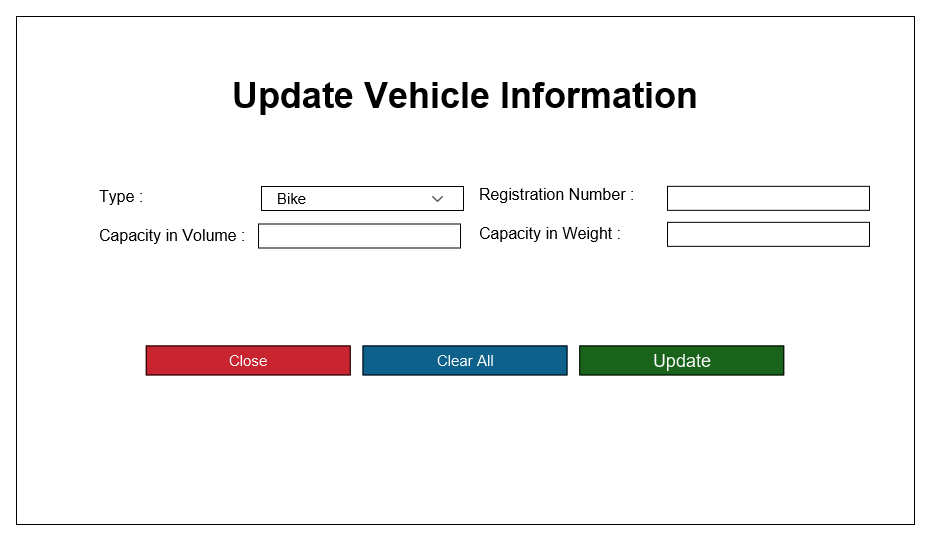
\includegraphics[scale=0.3]{./User Interface/UI-024 Update Vehicle Information.png}\end{center}  \\ \hline


Actual Interface in Visual Studio  & \begin{center} \includegraphics[scale=0.3]{./User Interface1/UI-024 Update Vehicle Information.png}\end{center}  \\ \hline

Validators & 
\begin{itemize}
\item   Registration number should contain alphabets and digits.
\item  Capacity in volume should be be numeric and positive. 
\item Capacity in weight should be be numeric and positive. 
\item All required fields must be filled correctly. 

\end{itemize}
\\ \hline
\end{longtable}
%------------------------------------------
\subsection{Add Category}
\begin{longtable}{| p{3cm}|p{12cm}|}
\multicolumn{2}{c}{}
\endfirsthead
\multicolumn{2}{c}{\tablename\ \thetable\ -- \textit{Continued from previous page}}\\
\multicolumn{2}{c}{}\\
\hline
\endhead
\hline \multicolumn{2}{r}{\tablename\ \thetable\ -- \textit{Continued on next page}} \\
\endfoot
\hline
\endlastfoot
\hline

Interface ID & I26  \\\hline

Name  &  Add Category \\ \hline

Linked Use Case & U11	 \\ \hline

UI Interface in JUSTINMIND & \begin{center} \includegraphics[scale=0.3]{./User Interface/UI-025 Add Category@1x.png}\end{center}  \\ \hline

Actual Interface in Visual Studio  & \begin{center} \includegraphics[scale=0.3]{./User Interface1/UI-025 Add Category@1x.png}\end{center}  \\ \hline

Validators & 
\begin{itemize} 
\item Category should contain alphabets.
\item Field must be filled correctly. 
\end{itemize}
\\ \hline
\end{longtable}
%------------------------------------------
\subsection{Update Category Information}
\begin{longtable}{| p{3cm}|p{12cm}|}
\multicolumn{2}{c}{}
\endfirsthead
\multicolumn{2}{c}{\tablename\ \thetable\ -- \textit{Continued from previous page}}\\
\multicolumn{2}{c}{}\\
\hline
\endhead
\hline \multicolumn{2}{r}{\tablename\ \thetable\ -- \textit{Continued on next page}} \\
\endfoot
\hline
\endlastfoot
\hline

Interface ID & I27  \\\hline

Name  &  Update Category Information \\ \hline

Linked Use Case & U12	 \\ \hline

UI Interface in JUSTINMIND & \begin{center} \includegraphics[scale=0.3]{./User Interface/UI-026Update Category Inofrmation@1x.png}\end{center}  \\ \hline

Actual Interface in Visual Studio & \begin{center} \includegraphics[scale=0.3]{./User Interface1/UI-026Update Category Inofrmation@1x.png}\end{center}  \\ \hline

Validators & 
\begin{itemize}
\item Category should contain alphabets.
\item Field must be filled correctly. 
\end{itemize}
\\ \hline
\end{longtable}
%------------------------------------------
\subsection{Add Vendor}
\begin{longtable}{| p{3cm}|p{12cm}|}
\multicolumn{2}{c}{}
\endfirsthead
\multicolumn{2}{c}{\tablename\ \thetable\ -- \textit{Continued from previous page}}\\
\multicolumn{2}{c}{}\\
\hline
\endhead
\hline \multicolumn{2}{r}{\tablename\ \thetable\ -- \textit{Continued on next page}} \\
\endfoot
\hline
\endlastfoot
\hline

Interface ID & I28  \\\hline

Name  &  Add Vendor \\ \hline

Linked Use Case & U13	 \\ \hline

UI Interface in JUSTINMIND & \begin{center} \includegraphics[scale=0.3]{./User Interface/UI-027Add Vendor@1x.png}\end{center}  \\ \hline


Actual Interface in Visual Studio  & \begin{center} \includegraphics[scale=0.3]{./User Interface1/UI-027Add Vendor@1x.png}\end{center}  \\ \hline

Validators & 
\begin{itemize}
\item   Vendor name and company name must be a alphabetic and word.
\item   Phone number and land line number must be number and no use of special character used. 
\item All required fields must be filled correctly. 
\end{itemize}
\\ \hline
\end{longtable}
%------------------------------------------
\subsection{Update Vendor Information}
\begin{longtable}{| p{3cm}|p{12cm}|}
\multicolumn{2}{c}{}
\endfirsthead
\multicolumn{2}{c}{\tablename\ \thetable\ -- \textit{Continued from previous page}}\\
\multicolumn{2}{c}{}\\
\hline
\endhead
\hline \multicolumn{2}{r}{\tablename\ \thetable\ -- \textit{Continued on next page}} \\
\endfoot
\hline
\endlastfoot
\hline

Interface ID & I29  \\\hline

Name  &  Update Vendor Information \\ \hline

Linked Use Case & U14	 \\ \hline

UI Interface in JUSTINMIND & \begin{center} \includegraphics[scale=0.3]{./User Interface/UI-028 Update Vendor Information@1x.png}\end{center}  \\ \hline


Actual Interface in Visual Studio  & \begin{center} \includegraphics[scale=0.3]{./User Interface1/UI-028 Update Vendor Information@1x.png}\end{center}  \\ \hline

Validators & 
\begin{itemize}
\item   Vendor name and company name must be a alphabetic and word.
\item   Phone number and land line number must be number and no use of special character used. 
\item All required fields must be filled correctly. 
\end{itemize}
\\ \hline
\end{longtable}
%------------------------------------------
\subsection{Add Stock}
\begin{longtable}{| p{3cm}|p{12cm}|}
\multicolumn{2}{c}{}
\endfirsthead
\multicolumn{2}{c}{\tablename\ \thetable\ -- \textit{Continued from previous page}}\\
\multicolumn{2}{c}{}\\
\hline
\endhead
\hline \multicolumn{2}{r}{\tablename\ \thetable\ -- \textit{Continued on next page}} \\
\endfoot
\hline
\endlastfoot
\hline

Interface ID & I30  \\\hline

Name  & Add Stock\\ \hline

Linked Use Case & U15	 \\ \hline

UI Interface in JUSTINMIND & \begin{center} \includegraphics[scale=0.3]{./User Interface/UI-029Add Stock.png}\end{center}  \\ \hline

Actual Interface in Visual Studio  & \begin{center} \includegraphics[scale=0.3]{./User Interface1/UI-029Add Stock.png}\end{center}  \\ \hline

Validators & 
\begin{itemize}
\item   Quantity,retail price and cost price must be number and no use of special character. 
\item All required fields must be filled correctly. 
\end{itemize}
\\ \hline
\end{longtable}
%------------------------------------------
\subsection{Update Stock Information}
\begin{longtable}{| p{3cm}|p{12cm}|}
\multicolumn{2}{c}{}
\endfirsthead
\multicolumn{2}{c}{\tablename\ \thetable\ -- \textit{Continued from previous page}}\\
\multicolumn{2}{c}{}\\
\hline
\endhead
\hline \multicolumn{2}{r}{\tablename\ \thetable\ -- \textit{Continued on next page}} \\
\endfoot
\hline
\endlastfoot
\hline

Interface ID & I31  \\\hline

Name  &Update Stock Information\\ \hline

Linked Use Case & U30	 \\ \hline

UI Interface in JUSTINMIND & \begin{center} \includegraphics[scale=0.3]{./User Interface/UI-030Update Stock Information.png}\end{center}  \\ \hline

Actual Interface in Visual Studio & \begin{center} \includegraphics[scale=0.3]{./User Interface1/UI-030Update Stock Information.png}\end{center}  \\ \hline

Validators & 
\begin{itemize}
\item   Quantity,retail price and cost price must be number and no use of special character. 
\item All required fields must be filled correctly. 
\end{itemize}
\\ \hline
\end{longtable}
%------------------------------------------
\subsection{Order Summary}
\begin{longtable}{| p{3cm}|p{12cm}|}
\multicolumn{2}{c}{}
\endfirsthead
\multicolumn{2}{c}{\tablename\ \thetable\ -- \textit{Continued from previous page}}\\
\multicolumn{2}{c}{}\\
\hline
\endhead
\hline \multicolumn{2}{r}{\tablename\ \thetable\ -- \textit{Continued on next page}} \\
\endfoot
\hline
\endlastfoot
\hline

Interface ID & I32  \\\hline

Name  &Order Summary\\ \hline

Linked Use Case & U34	 \\ \hline

UI Interface in JUSTINMIND & \begin{center} \includegraphics[scale=0.3]{./User Interface/UI-031 Order Summary@1x.png}\end{center}  \\ \hline

Actual Interface in Visual Studio  & \begin{center} \includegraphics[scale=0.3]{./User Interface1/UI-031 Order Summary@1x.png}\end{center}  \\ \hline

\end{longtable}
%------------------------------------------
\subsection{Order Detail}

\begin{longtable}{| p{3cm}|p{12cm}|}
\multicolumn{2}{c}{}
\endfirsthead
\multicolumn{2}{c}{\tablename\ \thetable\ -- \textit{Continued from previous page}}\\
\multicolumn{2}{c}{}\\
\hline
\endhead
\hline \multicolumn{2}{r}{\tablename\ \thetable\ -- \textit{Continued on next page}} \\
\endfoot
\hline
\endlastfoot
\hline

Interface ID & I33  \\\hline

Name  &Order Summary\\ \hline

Linked Use Case & U19	 \\ \hline

UI Interface in JUSTINMIND & \begin{center} \includegraphics[scale=0.3]{./User Interface/UI-032 Order Details@1x.png}\end{center}  \\ \hline

Actual Interface in Visual Studio & \begin{center} \includegraphics[scale=0.3]{./User Interface1/UI-032 Order Details@1x.png}\end{center}  \\ \hline



\end{longtable}
%------------------------------------------
\subsection{Add Company}
\begin{longtable}{| p{3cm}|p{12cm}|}
\multicolumn{2}{c}{}
\endfirsthead
\multicolumn{2}{c}{\tablename\ \thetable\ -- \textit{Continued from previous page}}\\
\multicolumn{2}{c}{}\\
\hline
\endhead
\hline \multicolumn{2}{r}{\tablename\ \thetable\ -- \textit{Continued on next page}} \\
\endfoot
\hline
\endlastfoot
\hline

Interface ID & I31  \\\hline

Name  &Add Company\\ \hline

Linked Use Case & U31	 \\ \hline

UI Interface in JUSTINMIND & \begin{center} \includegraphics[scale=0.3]{./User 
Interface/UI-033 Add Company @1x.png}\end{center}  \\ \hline


Actual Interface in Visual Studio & \begin{center} \includegraphics[scale=0.3]{./User 
Interface1/UI-033 Add Company @1x.png}\end{center}  \\ \hline

Validators & 
\begin{itemize}
\item   Contact number must be number and no use of special character used. 
\item   Name must be alphabetic.
\item All required fields must be filled correctly.
\end{itemize}
\\ \hline
\end{longtable}
%------------------Classes----------------------
%------------------------------------------
\section{Classes}
The classes which are used in the project are as under with there specific properties. 
\begin{center}
\addcontentsline{toc}{section}{}
\begin{longtable}{| p{4cm}|p{2cm}|p{2cm}|p{2cm}|p{3cm}|}
\multicolumn{5}{c}{}
\endfirsthead
\multicolumn{5}{c}{\tablename\ \thetable\ -- \textit{Continued from previous page}}\\
\multicolumn{5}{c}{}\\
\hline
\endhead
\hline \multicolumn{5}{r}{\tablename\ \thetable\ -- \textit{Continued on next page}} \\
\endfoot
\hline
\endlastfoot
\hline
\textbf {Class Name} & \textbf{ Software/ Domain }&\textbf {Is Abstract (Yes/No)}&\textbf{ Is Singleton (Yes/No)} &\textbf {Is the class will has parametrized constructor(Yes/No)}\\ \hline
 CEO 		&Domain			&No			&No	&Yes\\ \hline
 Company		&Domain			&No		&No	&Yes\\ \hline
 Office		&Domain			&No			&No	&Yes\\ \hline
 WareHouse	&Domain			&No			&No	&Yes\\ \hline
 User		&Domain			&No			&No		&Yes\\ \hline
 Rider		&Domain			&No			&No		&Yes\\ \hline
 Employee  	&Domain			&No			&No		&Yes\\ \hline
 WareHouseManager&Domain		&No		&No 	&Yes\\ \hline
 ShopOwner 	&Domain			&No			&No		&Yes\\ \hline
 Shop	  	&Domain			&No			&No		&Yes\\ \hline
 Ledger	  	&Domain			&No			&No	&Yes\\ \hline
 Order		&Domain			&No			&No		&Yes\\ \hline
 Product		&Domain			&No		&No		&Yes\\ \hline
 Vehicle		&Domain			&No		&No		&Yes\\ \hline
 Linked List	&Software		&No		&No		&Yes\\ \hline
 Array List &Software	&No		&No		&Yes\\ \hline
 Hash Table &Software	&No		&No		&Yes\\ \hline
 Graph  &Software		&No		&No		&Yes\\  \hline
\end{longtable}
\end{center}
%------------------------------------------------------------
%---------------Object Oriented Features---------------------
\section{Object Oriented Features}
\subsection{Composition}
In our Project there are 8 places where we use Composition
\begin{itemize}
\item   Company Class has composition of Ledger Class
\item  Company Class has composition of Office Class
\item  Company Class has composition of Warehouse Class
\item  Company Class has composition of CEO Class
\item  Warehouse Class has composition of  Warehouse Manager Class
\item  Rider Class has composition of Vehicle Class
\item  Office Class has composition of User Class ( Employee, Rider)
\item  Shop Owner Class has composition of Shop Class
\end{itemize}
\subsection{Inheritance}
In our project inheritance is used in following places
\begin{itemize}
\item   User inherits the class of CEO
\item User inherits the class of Rider 
\item User inherits the class of Shopkeeper
\item User inherits the class of Warehouse Manager  
\end{itemize}
\subsection{Multi-Level Inheritance}
In our project Multilevel inheritance is used as
\begin{itemize}
\item User class inherits the CEO class and CEO class inherits the Employee Class
\end{itemize}
\subsection{Aggregation}
In our project Multilevel inheritance is used as
\begin{itemize}
\item Rider Aggregate the Rating Class in our project
\end{itemize}
\subsection{Association}
In our project Multilevel inheritance is used as
\begin{itemize}
\item Warehouse Manager manages the order.
\item CEO manages the products
\item Rider take the order 
\item Rider adds the order
\item Employee adds the products
\item Employee manages the order 
\end{itemize}

%------------------Class Diagram--------------------
\section{Detailed Object Oriented Design}
\begin{figure}
  \centering
    \includegraphics[scale=0.8]{Image.jpg}
  \caption{The detailed Object Oriented Design of the project that will be implemented according to mentioned logic}
\end{figure}
\newpage
%------------------------------------
%------------------Data Structure--------------------
\section{Data Strucuture}
The following section shows the reason for choosing the data structure in the particular use case with a brief explanation.
%-------------------------------------------------------
\subsection{Linked List}
\begin{longtable}{| p{3cm}|p{12cm}|}
\multicolumn{2}{c}{}
\endfirsthead
\multicolumn{2}{c}{\tablename\ \thetable\ -- \textit{Continued from previous page}}\\
\multicolumn{2}{c}{}\\
\hline
\endhead
\hline \multicolumn{2}{r}{\tablename\ \thetable\ -- \textit{Continued on next page}} \\
\endfoot
\hline
\endlastfoot
\hline
\textbf{Use Case IDs}& U01,U02,U03,U04,U05,U06,U07,U08,U09,U010,U13,U14,
U15,U16,U17,U18,U19,U20,U21,U22,U25,U26,U27,U28,
U30,U31,U32,U33,U34,U35,
U36,U37,U38,U39,U40,U41,U42
 \\ \hline
\textbf{Data Structure Used}& Linked List \\ \hline

\textbf{Time Complexity}& 
In Worst Case: Search: O(n), Insertion: O(1), Deletion: O(n)\\\hline
\textbf{Space Complexity}& O(n)\\\hline
\textbf{Justification for the use of data structure}&
In mentioned use case required a linear-dynamic data structure. 
Doubly Linked List provides an efficient way to search the specific information from a large amount of data and then compare it with input information to produce the required result. It helps to store and delete the data fastly. It allows you to move back and forth in the list to get the required result.\\ \hline
\textbf{Pseudocode}& 
\textbf{Search:} \\&
LIST-SEARCH(L,k)\\&
1 x=L.head\\&
2 while x $\neq$ NIL and x:key $\neq$ k \\&
3\hspace{6 mm} x = x.next\\&
4 return x\\&
\textbf{Insert:} \\&
LIST-INSERT(L, x) \\&
1 x.next=L.head \\&
2 if L.head $\neq$ NIL \\&
3\hspace{6 mm} L.head.pre = x \\&
4 L.head = x \\&
5 x.pre = NIL \\&
\textbf{Delete:} \\&
LIST-DELETE(L,x)\\&
1 if x.pre $\neq$ NIL\\&
2\hspace{6 mm} x.pre.next=x.next\\&
3 else L.head D x.next\\&
4 if x.next $\neq$ NIL\\&
5\hspace{6 mm} x.next.pre =x.pre
 \\ \hline

\textbf{Available choices}& Array List,Hash Table \\ \hline
\textbf{Comparison}&
The array list worst and average case time complexity is O(n). It takes contiguous memory. The hash table is best in the average case, but in the worst case time, complexity rise to O(n). It takes contiguous memory for storing the hash function value. In the average and worst case, the linked list insertion and deletion take O(1) time. In the average and worst case, it takes O(n) time for deletion. It did not require contiguous memory allocation.Array list, hash table, and linked list space complexity O(n) are the same.
\\ \hline
\end{longtable}

%-------------------------------------------------------

%-------------------------------------------------------
\subsection{Array List}
\begin{longtable}{| p{3cm}|p{12cm}|}
\multicolumn{2}{c}{}
\endfirsthead
\multicolumn{2}{c}{\tablename\ \thetable\ -- \textit{Continued from previous page}}\\
\multicolumn{2}{c}{}\\
\hline
\endhead
\hline \multicolumn{2}{r}{\tablename\ \thetable\ -- \textit{Continued on next page}} \\
\endfoot
\hline
\endlastfoot
\hline
\textbf{Use Case IDs}& U11,U12,U29 \\ \hline
\textbf{Data Structure Used}& Array List \\ \hline

\textbf{Time Complexity}& 
In Worst Case: Search: O(n), Insertion: O(1), Deletion: O(n)\\\hline
\textbf{Space Complexity}& O(n)\\\hline
\textbf{Justification for the use of data structure}&
In mentioned use case required a linear-dynamic data structure. 
Array List provides an efficient way to search the specific information from a large amount of data and then compare it with input information to produce the required result.IT allows to get specific data and shows  the required result.Only a specific detail of the data is required to store the specific information in this use case. 
\\ \hline
\textbf{Available choices}& Linked List \\ \hline
\textbf{Comparison}&
The array list worst and average case time complexity is O(n). In the average and worst case, the linked list insertion and deletion take O(1) time. IN the average and worst case, List takes O(n) time for deletion. It did not require contiguous memory allocation.Array list and linked list space complexity O(n) are the same therefore for the small data Array list used.\\ \hline
\end{longtable}
%-------------------------------------------------------
\subsection{Hash Table}
\begin{longtable}{| p{3cm}|p{12cm}|}
\multicolumn{2}{c}{}
\endfirsthead
\multicolumn{2}{c}{\tablename\ \thetable\ -- \textit{Continued from previous page}}\\
\multicolumn{2}{c}{}\\
\hline
\endhead
\hline \multicolumn{2}{r}{\tablename\ \thetable\ -- \textit{Continued on next page}} \\
\endfoot
\hline
\endlastfoot
\hline
\textbf{Use Case IDs}& U23,U24 \\ \hline
\textbf{Data Structure Used}& Hash Table \\ \hline

\textbf{Time Complexity}& 
In Worst Case: Search: O(n), Insertion: O(n), Deletion: O(n)\\\hline
\textbf{Space Complexity}& O(n)\\\hline

\textbf{Justification for the use of data structure}&
In mentioned use case required a Hash Table data structure. 
Hash Table provides an efficient way to search the specific information from a moderate and huge amount of data and then compare it with input information to produce the required result. It allows to get specific data of some specific data, it allows to apply specific operation on that and shows the required result.\\ \hline
\textbf{Pseudocode}& 
\textbf{Insert:} 

HASH-INSERT(T,k)

1 i = 0

2 repeat

3\hspace{6 mm} j = h(k,i)

4\hspace{6 mm} if T[j]== NIL

5\hspace{12 mm} T[j]= k

6\hspace{12 mm} return j

7\hspace{6 mm} else i = i +1 

8 until i == m

9 error “hash table overflow”

\textbf{Search:} 

HASH-SEARCH(T,k)

1 i = 0

2 repeat

3\hspace{6 mm} j = h(k,i)

4\hspace{6 mm} if T[j]== NIL

5\hspace{12 mm} return j

6\hspace{6 mm} i=i+1

7 until T[j] == NIL or i==m

9 return NIL

\textbf{Search:} 

Remove(T,k)

1 i = h(k)

2 while A[j] $\neq$ NULL do 

3\hspace{6 mm} if A[j].key =k then

4\hspace{12 mm} temp=A[i]

5\hspace{12 mm} A[i]=NULL

6\hspace{12 mm} Call Shift(i) to restore A to a stable state without k

7\hspace{6 mm} return temp

9 i=(i+1) mode N

10 return null

\\\hline
\textbf{Available choices}& Linked List \\ \hline
\textbf{Comparison}&
The Hash Table worst and average case time complexity is O(n). In the average and worst case, the linked list insertion and deletion take O(1) time. IN the average and worst case, List takes O(n) time for deletion. It did not require contiguous memory allocation.Heap and linked list space complexity O(n) are the same therefore for the Detailed  data Heap used.
\\ \hline
\end{longtable}
%-------------------------------------------------------

%-------------------------------------------------------
\subsection{Graph}
\begin{longtable}{| p{3cm}|p{12cm}|}
\multicolumn{2}{c}{}
\endfirsthead
\multicolumn{2}{c}{\tablename\ \thetable\ -- \textit{Continued from previous page}}\\
\multicolumn{2}{c}{}\\
\hline
\endhead
\hline \multicolumn{2}{r}{\tablename\ \thetable\ -- \textit{Continued on next page}} \\
\endfoot
\hline
\endlastfoot
\hline

\textbf{Use Case IDs}& U29 \\ \hline
\textbf{Data Structure Used}& Graph \\ \hline

\textbf{Time Complexity}& 
In Worst Case: Search: O(lg n), Insertion: O( lg n), Deletion: O(lg n)\\\hline
\textbf{Space Complexity}& O(n)\\\hline
\textbf{Justification for the use of data structure}&
In mentioned use case required a Tree data structure. 
Tree provides an efficient way to search the specific information from a moderate and huge amount of data and then compare it with input information to produce the required result. It allows to plot the data and apply operation on the data to show the required result.\\ \hline
 \textbf{Pseudocode}& 
 
\textbf{Intitialize-Single-Source:} 

INITIALIZE-SINGLE-SOURCE(G,s)

1 for each vertex $v \in G.V$

2\hspace{6 mm} v.d = $\infty$

3\hspace{6 mm} v.$\pi$= Nil

4 s.d =0
 
 
 
\textbf{Relax:} 

RELAX(u,v,w)

1 if v.d $>$ w(u,v)

2\hspace{6 mm} v.d=u.d+w(u,v)

3\hspace{6 mm} v.$\pi$=u
 
\textbf{Bellman Ford:} 

BELLMAN-FORD(G,w,s )

1 INITIALIZE-SINGLE-SOURCE(G,S)

2 for i = 1 to $|G.V|$-1

3\hspace{6 mm} for each edge (u,v) $\in G.V$

4\hspace{12 mm} RELAX(u,v,w)

5 for each edge (u,v) $\in G.V$

6\hspace{6 mm} if v.d $>$ u.d+w(u,v)

7\hspace{12 mm} return FALSE

8 return TRUE

 \\ \hline
\textbf{Available choices}& Tree \\ \hline
\textbf{Comparison}&
The Graph worst and average case time complexity is O(lg n). In the average and worst case, the Tree insertion and deletion take O(lg n) time. IN the average and worst case, Tree takes O(n) time for deletion. It did not require contiguous memory allocation.Tree and Graph space complexity O(n) are  same therefore, for the Plotting  data graph is prefered to be used.
 \\ \hline
 \end{longtable}
 %---------------------------------------------------------
%-----------------------Exceptions-----------------------------


\section{Exceptions}
\begin{longtable}{| p{2cm}|p{5cm}|p{3cm}|p{4cm}|}
\multicolumn{4}{c}{}
\endfirsthead
\multicolumn{4}{c}{\tablename\ \thetable\ -- \textit{Continued from previous page}}\\
\multicolumn{4}{c}{}\\
\hline
\endhead
\hline \multicolumn{4}{r}{\tablename\ \thetable\ -- \textit{Continued on next page}} \\
\endfoot
\hline
\endlastfoot
\hline
\textbf{Type of Exception} & \textbf{Why this exception will occur} &\textbf{ Use Case Id in which exception could be occurred} & \textbf{How you will handle the} exception \\  \hline
Incorrect Format & By default system, take all input in string and the deploy system need to convert into desire format. If the input data is not converted into other datatype like int and float the future task not performed e.g. string 2 and int 2 behave different in CPU.

& U02 U03 U04 U04 U05 U05 U06 U7 U08 U09 U11 U13 U14 U19 U20 U21 U22 U23 U24 U25 U26 U27 U28 U29 U30 U33 U34 U35 U36 U37 U38 U39 U40 U40 U41
&Restrict the user to enter the required data in correct format.                      \\  \hline
File not Loaded & File not found or b. & U6 U10 U11 U15 U32 &Error msg will be shown and give option to user to enter correct path of the file.   \\  \hline
Stack OverFlow & When the data is more used than the assigned memory or b. & Almost All UIs except Dashboards &Error msg will be shown and give option to user to enter correct operation.   \\  \hline
Index Out Of Range Exception & when an invalid index is used to access a member of an array or a collection & All add ,update and view UIs.& Error msg will be shown. \\  \hline
\end{longtable}

%---------------------------------------------------------
%--------------------Data Storage-------------------------
\section{Data Storage}

\subsection{Users (CSV)}

Columns data names are
\begin{enumerate}
\item Designation 
\item Name 
\item Gender
\item CNIC number
\item Email address
\item Contact Number
\item Home Address
\item Username 
\item Password 
\item Assigned 
\end{enumerate}

\subsection{Warehouse (CSV)}

Columns data names are
\begin{enumerate}
\item Name			
\item TotalSpace		
\item CurrentSpace 	
\item OccupiedSpace 	
\item Latitude 		
\item Longitude 		
\item Area			
\item City			
\item State			

\end{enumerate}

\subsection{Company (TXT)}

Columns data names are
\begin{enumerate}
\item Name 	
\item Address
\item Phone 	
\item Revenue

\end{enumerate}


\subsection{Category (CSV)}
Columns data names are
\begin{enumerate} 
\item Category
\end{enumerate}

\subsection{Products (CSV)}

Columns data names are
\begin{enumerate}
\item Name 			
\item SKUNumber 		
\item Weight 			
\item Volume 			
\item SensitivityType 
\item Category 		
\item Manufacturer	

\end{enumerate}

\subsection{Vendors (CSV)}

Columns data names are
\begin{enumerate}
\item Name  			
\item ConcernedPerson 	
\item LandLine			
\item Contact 			
\item Amount 

\end{enumerate}


\subsection{Stocks (CSV)}
Columns data names are
\begin{enumerate} 
\item Productname 		
\item 	Quantity 			
\item 	Retailprice 		
\item 	Costprice 			
\item  	Manufacturingdate 	
\item  	Expirydate 			
\item 	 Recieveddate 		
\item 	Vendorname 			
\item Product 				
\item Vendor 			

\end{enumerate}


\subsection{ShopKeepers (CSV)}
Columns data names are
\begin{enumerate} 
\item 	ShopName 
\item ShopCity 
\item ShopArea 
\item ShopState

\end{enumerate}

\subsection{City (CSV)}
Columns data names are
\begin{enumerate} 
\item Name
\end{enumerate}


\subsection{Orders (CSV)}

Columns data names are
\begin{enumerate}
\item ShopkeeperName
\item OrderID 		
\item Orderstatus 	
\item ShopName 	
\item AssignedRider 

\item Name		 
\item Category 		
\item SKUNumber 		
\item Volume 		 
\item Weight 			
\item Manufacturer 
\item SensitivityType	


\end{enumerate}

\subsection{Vehicles (CSV)}
Columns data names are
\begin{enumerate}
\item vehicleType			
\item vehicleWeight		
\item vehicleVolume 		
\item registrationNumber	
\item assigned 			

\end{enumerate}



\subsection{Ledgers (CSV)}
Columns data names are
\begin{enumerate}
\item Paymenttype 			
\item Paymentmode 			
\item Currentdate 			
\item Amount 				
\item Bydesignation 		
\item Byname 				
\item Receivedbydesignation
\item Receivedbyname 		
\item Description 	

\end{enumerate}


\subsection{Routes (CSV)}
Columns data names are
\begin{enumerate}
\item Distance 
\end{enumerate}



%-------------------------------------------------------------
%--------------------------Email-----------------------
\section{Email Sending}
\begin{enumerate}
\item When Rider registers the Shopkeeper.
 \begin{enumerate}
    \item An Email is send to the Employee.
    \item An Email is send to the Shopkeeper.
 \end{enumerate}

\item When Rider takes and add the order from the Shopkeeper.
 \begin{enumerate}
    \item An Email is send to the Employee.
    \item An Email is send to the Shopkeeper.
 \end{enumerate}

\item When Employee assigns order to the Rider.
 \begin{enumerate}
    \item An Email is send to the Rider
    \item An Email is send to the WareHouse Manager.
 \end{enumerate}

 \item When Rider adds payment from the Shopkeeper.
 \begin{enumerate}
    \item An Email is send to the Employee.
    \item An Email is send to the Rider.
 \end{enumerate}
 
 \item When Stock from the Vendor added.
 \begin{enumerate}
    \item An Email is send to the Vendor
    \item An Email is send to the Employee.
 \end{enumerate}

 \item When WareHouseManager ready the order.
 \begin{enumerate}
    \item An Email is send to the Rider
    \item An Email is send to the Employee.
 \end{enumerate}
 \end{enumerate}
%---------------------------------------------------------
%--------------------------Project Plan-----------------------
\section{Project Plan}
%---------------------------------------------------------
\begin{longtable}{| p{1cm}|p{4cm}|p{2cm}|p{3cm}|}
\multicolumn{4}{c}{}
\endfirsthead
\multicolumn{4}{c}{\tablename\ \thetable\ -- \textit{Continued from previous page}}\\
\multicolumn{4}{c}{}\\
\hline
\endhead
\hline \multicolumn{4}{r}{\tablename\ \thetable\ -- \textit{Continued on next page}} \\
\endfoot
\hline
\endlastfoot
\hline
\textbf{ Use Case Id }&\textbf{ Member Name}&\textbf{Due Date}&\textbf{Completion Date} \\ \hline
01& Syed Hashir 	&06/12/2022 &06/12/2022  \\ \hline
02& Kabir Ahmed	&06/12/2022 &06/12/2022  \\ \hline
03& M. Hamad Hassan&06/12/2022  &04/12/2022\\ \hline

04& Syed Hashir 	&07/12/2022  &07/12/2022  \\ \hline
05& Kabir Ahmed	&07/12/2022  &07/12/2022 \\ \hline
06& M. Hamad Hassan&07/12/2022 &05/12/2022 \\ \hline

07& Syed Hashir 	&08/12/2022 &08/12/2022  \\ \hline
08& Kabir Ahmed	&08/12/2022 &08/12/2022  \\ \hline
09& M. Hamad Hassan&08/12/2022  &06/12/2022\\ \hline

10& Syed Hashir 	&09/12/2022  &09/12/2022 \\ \hline
11& Kabir Ahmed	&09/12/2022  &09/12/2022 \\ \hline
12& M. Hamad Hassan&09/12/2022  &08/12/2022\\ \hline

13& Syed Hashir 	&10/12/2022  &10/12/2022 \\ \hline
14& Kabir Ahmed	&10/12/2022  &10/12/2022 \\ \hline
15& M. Hamad Hassan&10/12/2022 &10/12/2022 \\ \hline

16& Syed Hashir 	&10/12/2022   &10/12/2022\\ \hline
17& Kabir Ahmed		&11/12/2022  &11/12/2022 \\ \hline
18& M. Hamad Hassan&11/12/2022 &11/12/2022 \\ \hline

19& Syed Hashir 	&12/12/2022 &12/12/2022  \\ \hline
20& Kabir Ahmed		&12/12/2022 &12/12/2022  \\ \hline
21& M. Hamad Hassan&12/12/2022 &12/12/2022 \\ \hline

22& Syed Hashir 	&13/12/2022 &13/12/2022   \\ \hline
23& Kabir Ahmed		&13/12/2022   &13/12/2022\\ \hline
24& M. Hamad Hassan&13/12/2022 &13/12/2022 \\ \hline

25& Syed Hashir 	&14/12/2022  &15/12/2022 \\ \hline
26& Kabir Ahmed		&14/12/2022  &15/12/2022 \\ \hline
27& M. Hamad Hassan&14/12/2022  &15/12/2022\\ \hline


28& Syed Hashir 	&15/12/2022  &15/12/2022 \\ \hline
29& Kabir Ahmed		&15/12/2022  &15/12/2022 \\ \hline
30,31 & M. Hamad Hassan&15/12/2022  &15/12/2022\\ \hline

32& Syed Hashir		&16/12/2022  &16/12/2022 \\ \hline
33& Kabir Ahmed		&16/12/2022  &16/12/2022 \\ \hline
34& M. Hamad Hassan		&16/12/2022  &16/12/2022 \\ \hline

35& Syed Hashir		&17/12/2022  &19/12/2022 \\ \hline
36& Kabir Ahmed		&17/12/2022  &18/12/2022 \\ \hline
37& M. Hamad Hassan		&17/12/2022  &20/12/2022 \\ \hline

38& Syed Hashir		&18/12/2022  &21/12/2022 \\ \hline
39& Kabir Ahmed		&18/12/2022  &21/12/2022 \\ \hline
40& M. Hamad Hassan		&18/12/2022  &21/12/2022 \\ \hline

41& Syed Hashir		&19/12/2022  &20/12/2022 \\ \hline
41& Kabir Ahmed		&19/12/2022  &21/12/2022 \\ \hline
\end{longtable}

%--------------------------------------
%-------------------------Analytical Report-----------------
\section{Analytical Report}
%--------------------------------------------------------
In the system the created reports are:
\begin{enumerate}
\item Salary Report  
\item Rider Capture Order Report 
\item Profit Report 
\item Sold Products Report
\item Daily Stock Report 
\item Expenditure Report
\end{enumerate}
%---------------------------------------------------------
%---------------------------------------------------------
%---------------------------------------------------------
\end{document}